\chapter{Exoskeleton Controllers}
\label{chap:controllers}
\section{Introduction}
So far, a detailed pipeline has been presented, from the collection of human motion capture data to custom analysis tools to learning ideal motions. The final part is the model-based controller. The controllers build upon all the previously discussed work.  
Controllers are a key aspect of lower limb exoskeletons; they allow the exoskeleton to move through desired motions. Different controllers have been developed to control the motion of the exoskeleton and the human. A large aspect of these controllers is designed to consider the exoskeleton's dynamics model, allowing the non-linear dynamics to be canceled out when computing the control input. LARRE is assumed to be non-linear and modeled by \autoref{eq:Dyn} where $M$ is the mass-inertia matrix, $C$ is the Coriolis terms, $G$ is the gravity terms. This is similar to other models discussed in \cite{huo2016active} \cite{vantilt2019model}.

\begin{equation}
    \tau = M(q) \ddot{q} + C(q, \dot{q}) \dot{q} + G(q)
    \label{eq:Dyn}
\end{equation}


Several assumptions are made in the design of the controllers. First, the ground force reactions cannot be measured, which prevents feedback from the step. Second, human effort can be measured, and this is directly done through the simulation package. This measurement can be replicated on a physical exoskeleton using force sensing resistors or IMUs in the legs of the system. The force being applied by the user can be measured using the forces sensor embedded in the legs of the exoskeleton. By combining the measurement with the exoskeleton's kinematics model, the exerted torque can be estimated. Additionally, it is possible to use IMU to measure the angler acceleration and calculate the torque using an observer and a dynamics model. Third, the exoskeleton gait speed is slow. Gait training using an exoskeleton has been shown to improve the gait speed of people with paraplegia. The average walking speed after training was on average $0.43m/s$ \cite{khan2019retraining} compared to the average walking speed of a person is $1.5m/s$ \cite{fitzpatrick2006another}. A slow gait can be defined between $0.8-1.0m/s$. The expected gait speed is about half of the low end of a typical slow gait \cite{walsh2007quasi}; this means that the expected gait speed is on average less than $1/3$ of a normal gait speed. The average measured walking speed in LARRE was approximately $0.082m/s$, below what is considered a slow gait. These slow speeds reduce the sudden impact on the joints. 

Two different controllers are presented; the first is an iLQR controller, the second is a cooperative controller. The iLQR controller takes advantage of learning from demonstration and optimal controller theory to generate an optimal control signal to control the exoskeleton. Kirk defines optimal control as the method of finding a control signal that will cause a process to satisfy the physical constraints of and minimize some performance criterion \cite{kirk2004optimal}. The cooperative controller is designed to provide assistive control commands to combine the person's torques and the exoskeleton. It enables the exoskeleton only to provide the difference in torque between the required and what the person provides. The cooperative controller enables the user to provide any effort they are able to, and the exoskeleton provides the remaining effort. In doing so, the user will be engaged in the rehabilitation process; this can prompt healthy physical exercise for muscle growth and mental engagement in the rehabilitation.   

All the controllers are implemented using the control architecture discussed in \autoref{sec:controlarchitecture}—the modular control system allowed for controllers to be quickly implemented and tested. The RBDL library allowed for the fast computation of the dynamics of the exoskeleton allowing for real-time control. 

% The controller presented in \cite{martinez2017controller} was implemented on the Indigo exoskeleton and used a combination of force fields and human demonstration data to control the movement of the exoskeleton joints. This method did not consider the mass of dynamics of the exoskeleton and was designed to work on stroke patients with unilateral control. 


\section{iterative Linear Quadratic Regulator}
\label{sec:ilqr}

\subsection{Overview of iLQR Controller}
This work was published in IEEE Engineering in Medicine and Biology 43rd annual Conference \cite{goldfarb2021control}
The objective of this controller was to close the loop between the reproduction models and the controller. Current Learning from Demonstration (LfD) methods have been combined with linear quadratic regulators but not iterative linear quadratic regulators; this limits the applicability of processes since most robotic systems have non-linear dynamics. An iterative linear quadratic regulator is used to find an optimal control signal to drive the exoskeleton joints through the desired trajectories. The iLQR torque is used as a feed-forward term, with a PD controller added as a closed-loop component for unmodeled dynamics. The LfD trajectory is optimized using the Bayesian Information Criterion (BIC). This dissertation will show how the trajectory is learned, and the control signal is optimized by reducing the required bins for learning. The framework presented produces optimal control signals to allow the exoskeleton's legs to follow human motion demonstrations.

The Linear Quadratic Regulator (LQR) is a well-known method that provides optimally controlled feedback gains to enable the closed-loop and high-performance control \cite{kirk2004optimal}. The limitation of LQR is that it is intended to be implemented on a system with linear dynamics and has a linear cost function. In \cite{TPGMM_calinon2016}, Calinon \textit{et. al} used TPGMM/GMR with an LQR controller to develop a minimal intervention controller. This controller was used to control a Kuka robotic arm \cite{schreiber2010fast} through a series of movements. This method led to the inspiration to use a non-linear controller instead of the linear one used previously.  

The Iterative Linear Quadratic Regulator (iLQR) is a non-linear version of the LQR controller. The iLQR is an iterative process that uses a Taylor approximation of the dynamics and cost function to find a local linear model. The dynamics and cost function are linearized in the forward pass of the system using a shooting method, while like an LQR, the backward pass calculated the optimal gain and cost. Differential Dynamic Programming(DDP) is a similar method to iLQR; in classical DDP, the second-order terms are costly operations \cite{iLQR_tassa2014}  \cite{iLQR_Zachary2016}. 

This modification to LQR allows the control of non-linear system control problems; this is useful because it expands the systems the LQR can be applied to, including biological movement system \cite{iLQR_Li2004} and online trajectory optimization \cite{iLQR_tassa2012}. iLQR compared to ODE solvers, the iLQR gradient descent methods and differential dynamic programming converge substantially faster and find slightly better solutions \cite{iLQR_Li2004}. 

iLQR controllers have been implemented on a wide variety of systems. In \cite{car} they used a modified form of iLQR called constrained iLQR to control the motion of a car. The car was subjected to several state and control constraints. iLQR also allows for the control of humanoid robots. Tassa \textit{et. al} used iLQR to control an HRP-2 robot's motion by controlling the joint angles \cite{iLQR_tassa2014}.

\subsection{Methods and Implementation}
 The proposed approach is split into several phases; demonstration, encoding, and optimization. During the demonstration phase, gait data is collected, and the gait cycles are parsed to extract the joint angles. The demonstrations are encoded using TPGMM/GMR as discussed in \autoref{sec:lfd}. In the demonstration and encoding phases, the trajectories are learned and encoded. The controller is tested on the LARRE model in AMBF as discussed in \autoref{chap:sim}. 

The control inputs calculated drive the system along the trajectory during the optimization phase. There are two steps in the iLQR algorithm; a forward-pass and a backward-pass. The simulated LARRE is simulated forward along the trajectory using a dynamic model in the forward-pass.  \autoref{fig:ilqrDiagram} shows a diagram of how the iLQR algorithm works.


\begin{figure}[h]
    \centering
    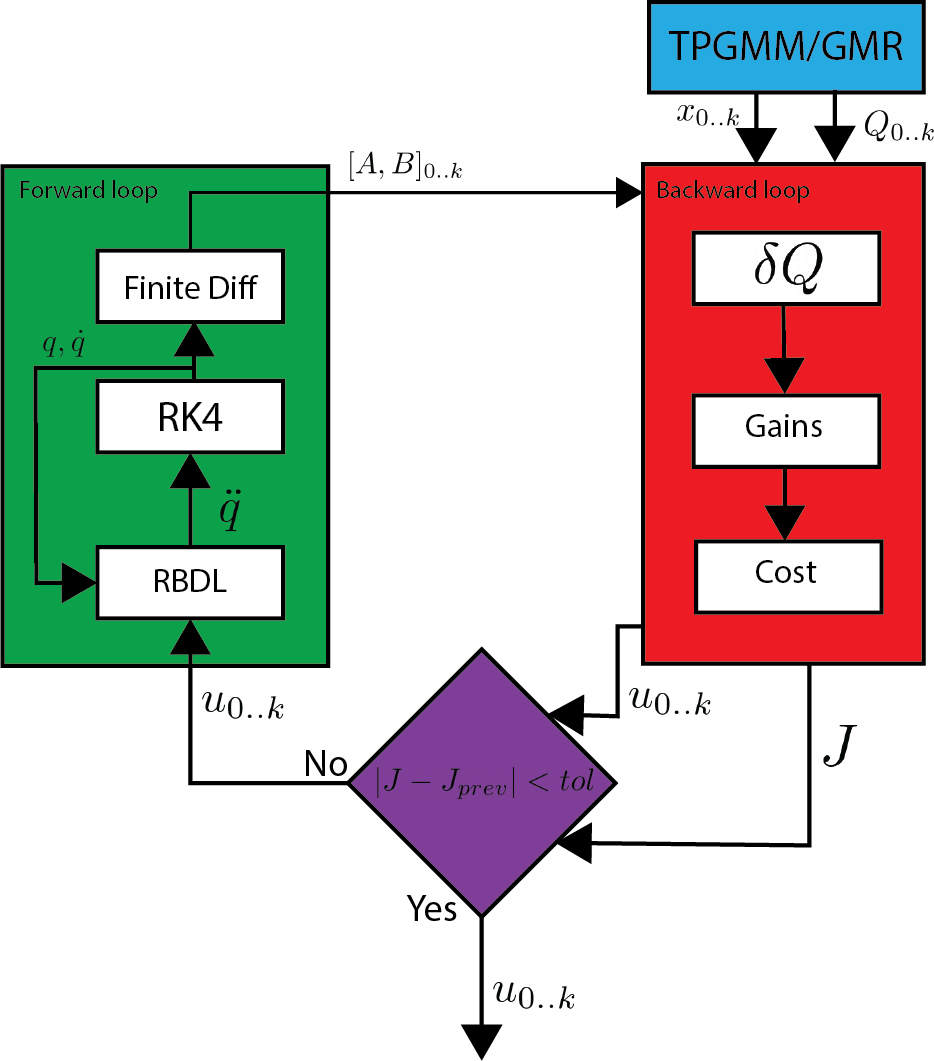
\includegraphics{images/controllers/ilqr2.png}
    \caption[iLQR Learning Loop Diagram]{Diagram of how the iLQR algorithm works with the forward pass and backward pass. The loop exists when the difference in current cost and previous cost is below a tolerance. }
    \label{fig:ilqrDiagram}
\end{figure}

Runge Kutta 4 (RK4) integrates the system forward to obtain the next state of the system \cite{dit2017runge} (See Appendix for implantation). RK4 is a numerical integration method that perturbs the system around a point and uses an average response average value. In the backward-pass, the system is solved backward to update the control parameters. A modified version of the \textit{ilqr} open-source library\footnote{https://github.com/anassinator/ilqr} was used and implemented. The modification allowed optimization along a pre-computed path with a variable $Qs$. This allows for the connection between Learning from Demonstration (LfD) and the controller to be made, which will be explained in the following sections. The algorithm iteratively continues back and forth until the cost $J$ converges, indicating that the control signal $u$ can drive the system along the desired trajectory. 

\autoref{eq:system_dyn} defines the  generalized non-linear system dynamics. The cost function is the sum of the running cost and the terminal cost shown in \autoref{eq:cost}. This paper uses a linear cost function to take advantage of the TPGMM/GMR process shown in \autoref{eq:mycost}, where $\tilde{x}_k = x_k - x^{d}_k$. This paper's cost function is designed to follow a reference trajectory $x^{d}$ using GMR. The $Q_k$ varies along the path and  are calculated by the TPGMM algorithm ($Q_k$ =  $\Sigma_k^{-1}$). The  $Q$ matrix is the weight for transitioning, and the $R$ matrix is the weight of the control. The calculation of the $Q$ and $R$ matrix will be addressed in the next section.

\begin{equation}
     x_{k+1} = f(x_k,u_k) 
     \label{eq:system_dyn}
\end{equation}

\begin{equation}
    J(x,U) = \ell_f (x_N) + \sum_{k=0}^{N-1} \ell(x_k, u_k) 
    \label{eq:cost}
\end{equation}

where,
\begin{equation}
    \begin{split}
            \ell(x_k, u_k) &= \tilde{x}_k^T Q_k \tilde{x}_k + u_k^T R u_k \\
    \ell_f(x_N) &= x^{T}_{N} Q_N x_{N}
    \end{split}
      \label{eq:mycost}
\end{equation}

The value function is found using \autoref{eq:value} which is minimized over the entire control sequence. $\ell (x,u)$ is the final cost and $V(f(x,u))$ is the cost-to-go, which is the cost associated with moving forward along the trajectory. Which is the Bellman principle of optimally. Using calculus of variations \autoref{eq:deltaQ} is calculated and decomposed \autoref{eq:deltaQDecomp}, where $ A =\partial f / \partial x$ and  $B = \partial f / \partial u$.  The particles derivatives are calculated in the forward pass at each time step using a finite difference method \cite{iLQR_Zachary2016}. 


\begin{equation}
    \begin{split}
        Q(x,u) &= \ell (x,u) + V(f(x,u)) \\
        V(x,u) &= \min\limits_{u} Q(x,u)
    \end{split}
    \label{eq:value}
\end{equation}


\begin{equation}
     \delta Q = 
     \frac{1}{2}
     \begin{bmatrix}
     1 \\
     \delta x \\
     \delta u
     \end{bmatrix}^T
       \begin{bmatrix}
        0       & Q^T_{x} & Q^T_{u}  \\
        Q_{x}   & Q_{xx} & Q_{xu}  \\
        Q_{u}   & Q_{ux} & Q_{uu} 
    \end{bmatrix}
    \begin{bmatrix}
     1 \\
     \delta x \\
     \delta u
     \end{bmatrix}
        \label{eq:deltaQ}
\end{equation}

\begin{equation}
    \begin{split}
        Q_x &= \ell_x + A^T V'_x \\
        Q_u &= \ell_u + B^T V'_x \\
        Q_{xx} &= \ell_{xx} + A^T V'_{xx}A \\
        Q_{uu} &= \ell_{uu} + B^T V'_{xx}B \\
        Q_{ux} &= \ell_{ux} + B^T V'_{xx}A \\
    \end{split}
    \label{eq:deltaQDecomp}
\end{equation}



The optimization finds the total cost and the optimal control gains for the system. The control sequence is found using \autoref{eq:control}, where $K=-Q_{uu}^{-1}Q_{ux}$ and $k=-Q^{-1}_{uu} Q_{ux}$. The $\alpha$ term is a linear search term to ensure convergence of the system, and $\hat{u}_k$ is the nominal control input. 


\begin{equation}
    u_k = K_k (x_k - \hat{x}_k) + \alpha k_k + \hat{u}_k
    \label{eq:control}
\end{equation}

One of the primary problems with iLQR is that it is difficult for real-time control. A Model Predictive Controller (MPC) could be used to solve some of the limitations of LQR \cite{bemporad2002explicit}. One of the main differences between LQR and MCP is that LQR is an infinite horizon controller and MPC is a finite horizon controller and has been used for real-time control \cite{wang2009model}. However, using iLQR instead of LQR becomes more difficult when attempting real-time control due to the computational time of the line search step, which cannot be done in real-time because it is unknown how many iterations this step will take. This limitation can somewhat be overcome by using parallel processing in a separate thread, which would run parallel to the main controller thread \cite{MPC}. This solution is equivalent to using more computing power and may not be a possible solution on all systems. If a better initial guess could be made, it is possible to reduce the line search loop; this would not work for all possible trajectories because of the difficulty of generalizing the initial guess for all possible trajectories. 


Because of real-time limitations, the control command is calculated offline and applied online due to the computational time for the forward and backward loops. The calculation can take up to several seconds or minutes depending on the degrees of freedom, length of trajectory, and computational power of the computer used to train. To circumvent this problem, a PD controller was added into the loop to allow for error tracking in real-time; the PD controller handles errors in un-modeled dynamics such as joint friction, and damping \cite{iLQR_tassa2014}. The iLQR torque acted as a feed-forward term driving the system, and the PD controller handled path deviation errors. \autoref{fig:controller} show the control diagram. 


\begin{figure}[H]
    \centering
    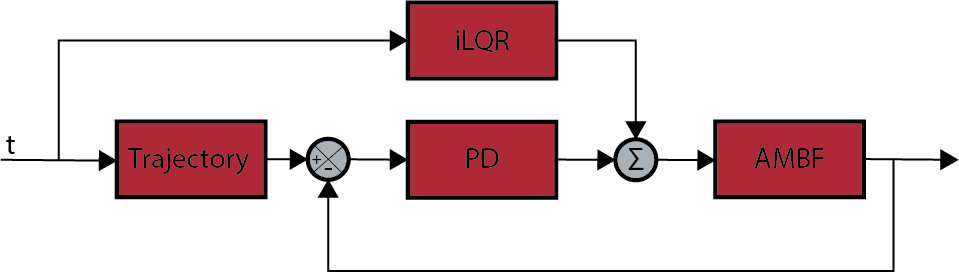
\includegraphics[width=\linewidth]{images/controllers/iLQR.png}
    \caption[iLQR Control Diagram]{Control diagram of the exoskeleton. The trajectory is found using TPGMM. The iLQR provides a feedforward control input. The PD controller removes un-modeled dynamics of the system }
    \label{fig:controller}
\end{figure}

As discussed above, the TPGMM process finds optimal values for the $Q_i$ along the trajectory, which is the weighting of the system's state. However, this does not provide insight into the value of the $R$ matrix, which is the weighting of the control input into the system. These values are critical because they determine the amount of effort applied at every point along the trajectory. The shape of the $R$ matrix for this application is $6 \times 6$ diagonal matrix.


The first three diagonal elements of the $R$ matrix are correlated to the control input of the left leg (\textit{hip}, \textit{knee}, \textit{ankle}). The other three diagonal elements are related to the control input of the right leg (\textit{hip}, \textit{knee}, \textit{ankle}). This paper assumes symmetry of the joints for the left and right legs i.e. $\textit{hip}_R$ == $\textit{hip}_L$.  This assumption is possible because each leg would have similar masses and be controlled with identical motors. In addition, the minor differences can be supplemented by the $Q$ matrix during the iLQR training.  

To find the $R$ matrix's values; the values were iteratively changed to find a matrix that minimizes cost $J$ defined in \autoref{eq:R_cost} which is the root mean squared error (RMS), where $N$ is the number of points for output, $x_i$ are the points on the desired joint trajectory, and $\hat{x_i}$ are the points on the actual trajectory; this is in joint space for each of the joints. 
 \cite{chai2014root}.

\begin{equation}
    J = \sqrt{\frac{\sum_{i=1}^N(x_i-\hat{x_i})^2}{N}}
    \label{eq:R_cost}
\end{equation}

The high dimensional and non-linear dynamics make it challenging to weight values of the matrix \cite{park2012multi}. The complexity of the motor behaviors also increases the difficulty of finding the $R$ matrix. Therefore, a brute-force method was implemented to go through values in different magnitudes and select the optimal result. The control signal was tested by forward integrating using RK4. The values of the $R$ matrix were incremented and the iLQR process was rerun and the control input was used to control the dynamic model and the resultant trajectory was saved and compared to the desired motion. The RMS error was measured and recorded. The values of $R$ that resulted in the lowest RMS error were used in the final controller. 
% \autoref{fig:error_digram} show the optimal trajectory and one unfit case:

% \begin{figure}[H]
%     \centering
%     \includegraphics[width=\linewidth]{Images/effor_2.png}
%     \caption{Joint Angles for the trajectories. The blue line is the desired motion, the red line is well fit trajectory, and the green line is a poorly fit trajectory.}
%     \label{fig:error_digram}
% \end{figure}

% Changing the values of the $R$ matrix significantly affects the replication of the trajectory. The $R$ matrix has to be tuned to replicate the desired trajectory.  

\subsection{Results and Discussion}



The path and $Qs$ are generated by the TPGMM/GMR process and initialize the iLQR controller algorithm. As the name implies, the iLQR algorithm is an iterative possesses that stops when the cost $J$ converges.  \autoref{fig:cost} shows the converges of the cost for each iteration. The cost coverage's from $\sim47.5 \rightarrow \sim27.5$ after 6 iterations. The convergence of the iLQR indicates the error between the desired and actual have been reduced, and the efforts along the trajectory have been minimized. 

 

\begin{figure}[h!]
    \centering
    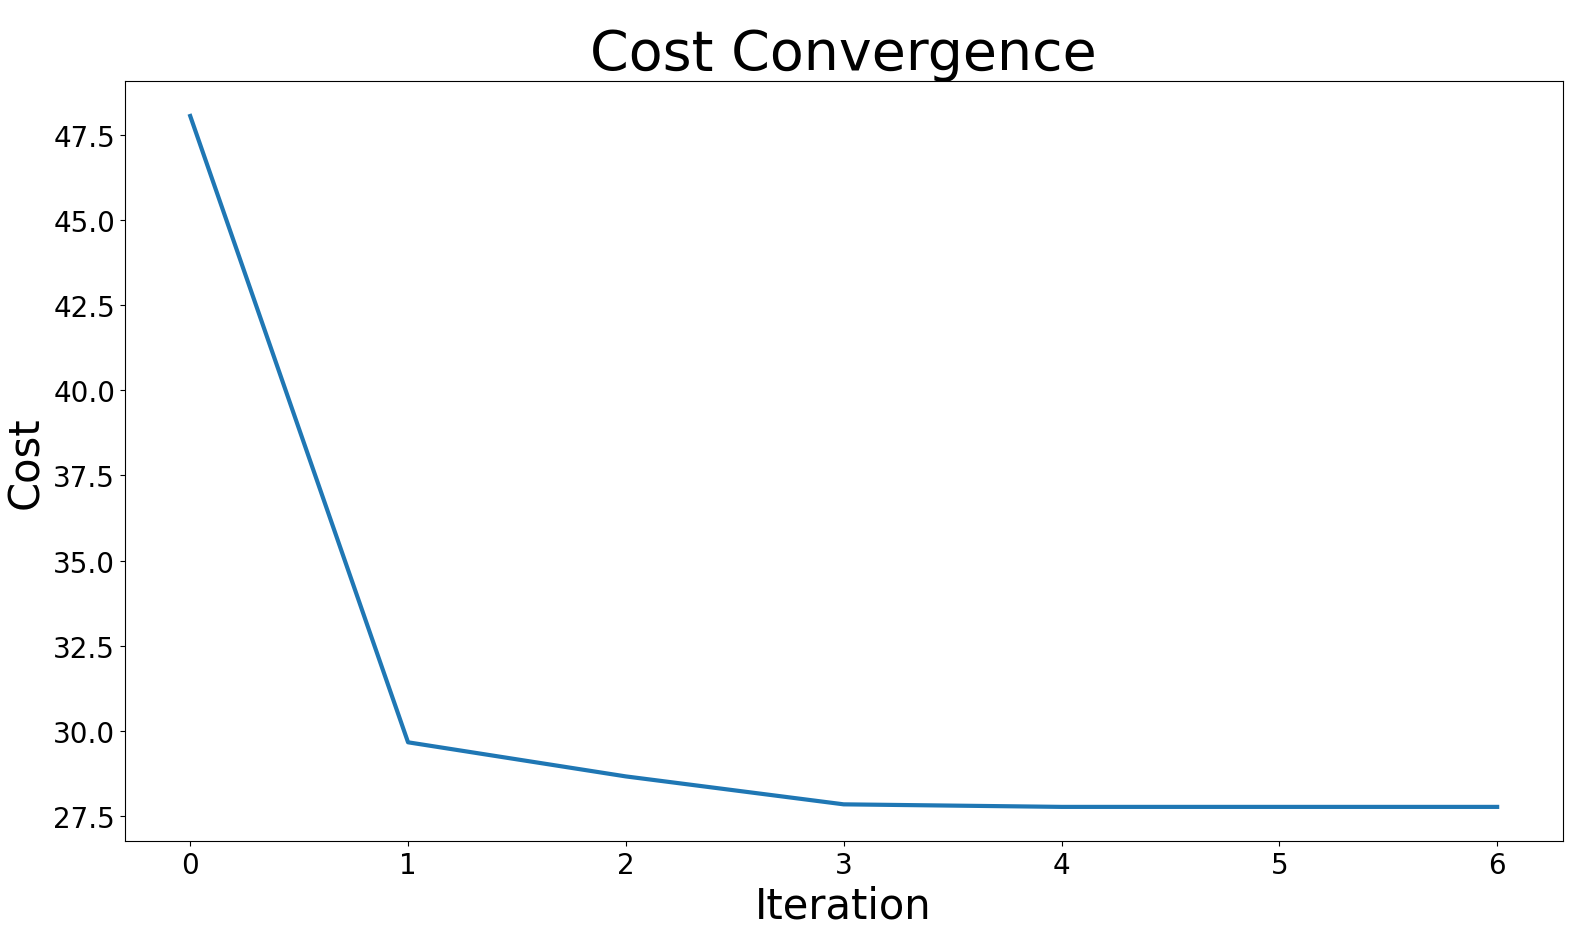
\includegraphics[scale=0.22]{images/controllers/Cost_plt3.png}
    \caption[iLQR controller Convergence]{Converges of the iLQR controller cost.}
    \label{fig:cost}
\end{figure}


\autoref{fig:comparison} shows a comparison of the exoskeleton joints to the reference trajectory. The orange line references the trajectory, and the blue line is the path the exoskeleton joints traveled. LARRE's joints were able to track the desired motion. 


\begin{figure}[h!]
    \centering
    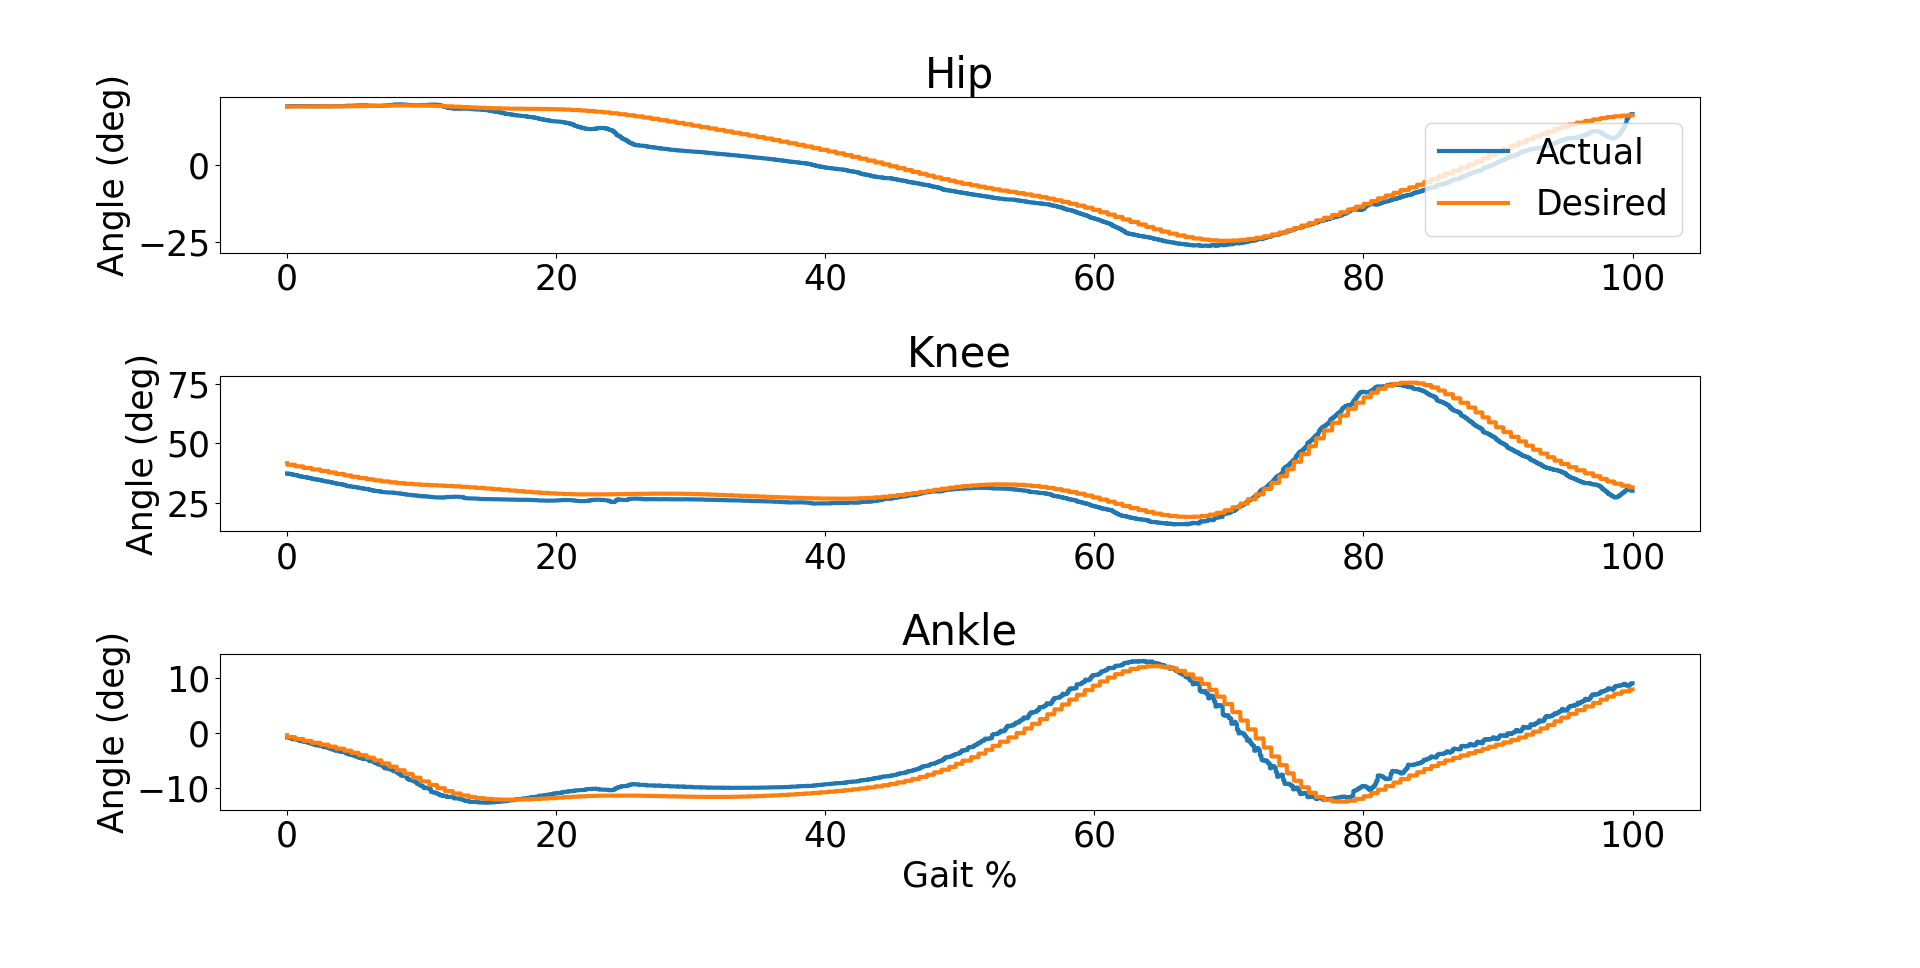
\includegraphics[scale=0.27]{images/controllers/compare_traj.png}
    \caption[iLQR controller trajectory]{Comparison of the actual joint angles to the reference trajectory.}
    \label{fig:comparison}
\end{figure}


\autoref{fig:comparisonTorque} shows a comparison of the joint effort over the trajectory. The iLQR feed forward term and the total torque (iLQR+PD) are presented. Additionally, the effort of a pure PD controller is presented for comparison of effort. This is not the same PD effort used for the total torque ( \textit{orange} +  \textit{green} $\neq$  \textit{blue} ). The iLQR term can closely follow the total torque indicating that most of the control command is provided from the iLQR controller, not the PD term. Additionally, the PD controller control input is noisy and has greater efforts than the iLQR control signal showing that the iLQR can produce lower torque than a PD controller. 

\begin{figure}[h!]
    \centering
    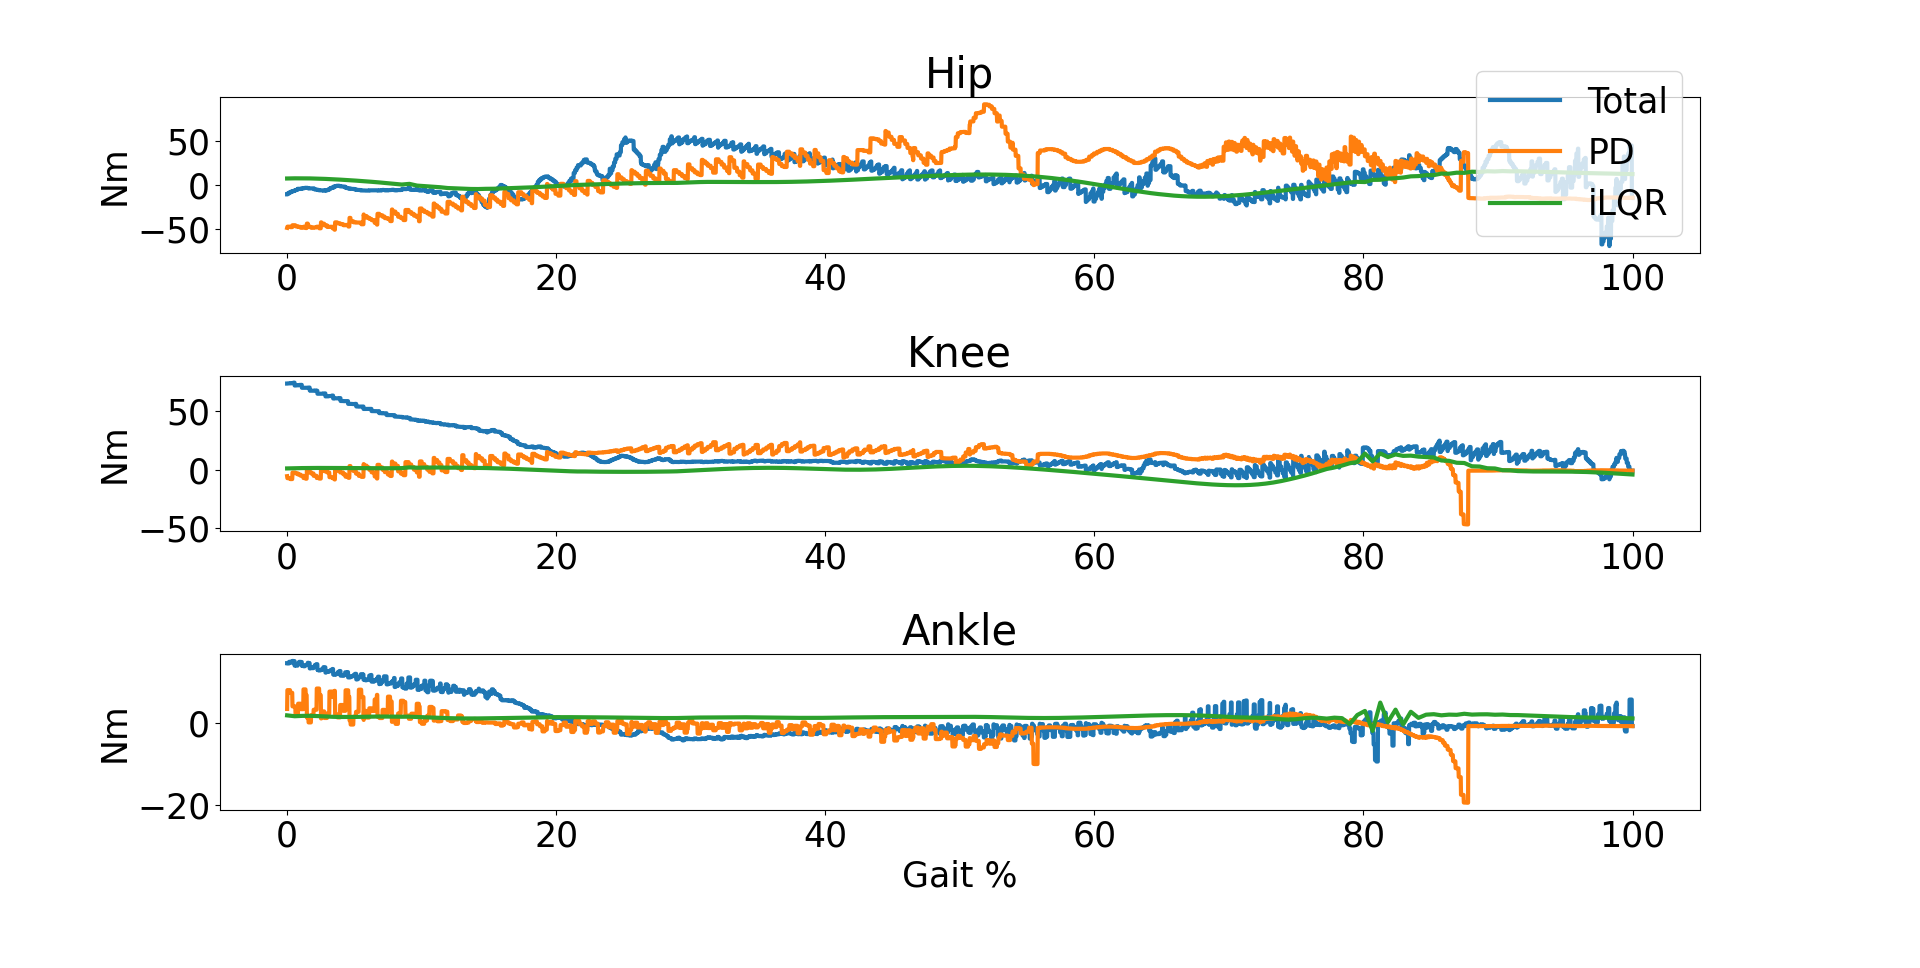
\includegraphics[scale=0.35]{images/controllers/torque_compare.png}
    \caption[Torque Comparison of the iLQR controller]{Comparison of the PD alone vs ILQR and iLQR feedforward + PD feedback}
    \label{fig:comparisonTorque}
\end{figure}



\section{Cooperative Controllers}


\subsection{Overview Cooperative Controllers}
Assistive controllers have long been implemented in rehabilitative exoskeletons. This includes the MIT-MANUS \cite{ju2005rehabilitation}, BLEEX\cite{kazerooni2006hybrid}, HAL\cite{kawamoto2004power} and many others robotic systems including several exoskeletons \cite{kim2012admittance,ott2010unified,huo2011control}. These systems use assistive controllers to help guide the person's arm or leg through a desired trajectory or to complete tasks. This method is typically used because the person has difficulty generating the necessary torques due to medical problems such as a stroke or spinal cord injury. The difficulty in designing these systems is in handling the non-linearity and distances from being connected to a person, which the controller will have to overcome. Many of these controllers implement either admittance or impedance models. Admittance controllers transform forces and torques to the desired position and orientation. Impedance controllers are the mirror to admittance controllers calculating displacements from applied forces and torques. Impedance controllers allow for virtual stiffness, which is useful for controlling the human-robot interactions \cite{keemink2018admittance}. 

The admittance controller has shown better results when implemented into an exoskeleton. They are easier to implement and can measure the intention of the user because movement is easier to measure then precises torques. Admittance controllers allow for the adjustment of the stiffness to meet the on-the-fly demand by either being more or less aggressive in the supplied force \cite{aguirre2007active,newman1994stable}. This problem is solved by using variable admittance, where the parameters are adjusted based on the user's intention and ability.

Oh \textit{et. al} proposed a generalized framework for assistive controllers \cite{oh2015generalized}. The proposed controller combined a model-based method with feed-forward disturbance rejection—this method models the interaction as a disturbance to the system instead of an interactive force.  Additionally, a Sliding Mode Controller (SMC) controller was used, in contrast to a PD, which has been shown to have better performance in controlling non-linear systems \cite{slotine1991applied}.


\subsection{Sliding Mode Controller}

SMC is a popular method in assistive controllers due to their insensitivity to disturbances and handling of non-linearity better than a traditional PD controller \cite{nasir2010performance} \cite{sanngoen2020review} \cite{fischer-SMC}. SMC works by using a switching function to drive the system along a sliding surface. Torabi \textit{et al.} used a model-based SMC controller to drive a lower limb exoskeleton. This controller also used an adaptive admittance controller along with the SMC to adjust to the user intention ability \cite{torabi2018robust}. A similar method of model-based SMC was used by Babaiasl \textit{et. al} to control an upper limb exoskeleton \cite{babaiasl2015sliding}.


A SMC controller can be defined using \autoref{eq:SMC} where, $e(t) = x_d(t) - x(t)$ and $\dot{e}(t) = \dot{x}_d(t) - \dot{x}(t)$. A major problem  is that the $sign$ function is not continuous, which causes high-frequency chatter along the sliding surface, which is undesirable. This problem can be solved by swapping out the $sign$  function for different functions, which will produce a smoother transition by defining a boundary layer around the sliding surface \cite{babaiasl2015sliding}. One such function is the $\tanh$ function, which is an approximation of the $sin$. The $\tanh$ is continuous with adaptive gains and steepness \cite{aghababa2012chattering}. The swapping of functions is is done by using $\tanh(\sigma / \beta)$ where $\beta$ is the width of the boundary layer; this can be specified for each individual joint. Here $\vec{\sigma}$ is the sliding manifold, which is a vector with a length equal to the joint space of the system. $\Lambda$ is a diagonal matrix that handles a system's response, which affects the controller's rise time. Finally, $\rho$ is also a diagonal matrix that handles eliminating the disturbance in the system, and this should be larger than the anticipated noise.  \autoref{eq:SMCcnrl} shows the model-based SMC controller.

\begin{equation}
   \begin{aligned} 
        \vec{\sigma} &=  \dot{e}  + \Lambda e \\
        \vec{u} &= \ddot{x}_d - \Lambda \dot{e} - \rho * sign(\vec{\sigma})
    \end{aligned}
    \label{eq:SMC}
\end{equation}






\begin{equation}
        \tau_{tor} = M(q) \Big( \ddot{q}_d  - \Lambda e - \rho \tanh(\frac{\sigma}{\beta}) \Big) + C( q, \dot{q} ) + G(q) 
    \label{eq:SMCcnrl}
\end{equation}






In \cite{long2016robust} a genetic algorithm was used to tune the parameters of an SMC for a lower limb exoskeleton. The parameters were tuned in MATLAB/SIMULINK. While successful, they did not model a connection between the human and the exoskeleton and did not use an adaptive admittance controller. 

\begin{figure}
    \centering
    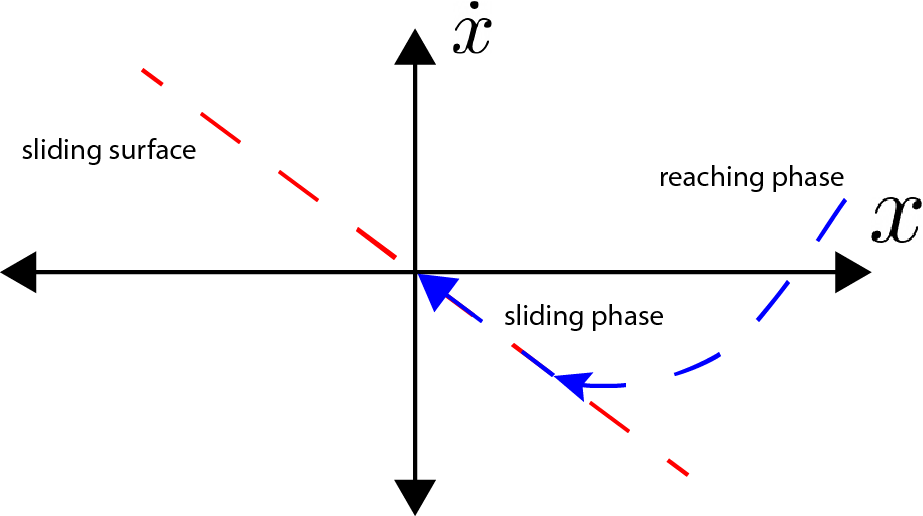
\includegraphics[width=\linewidth]{images/controllers/SMC.png}
    \caption{Sliding mode control and the switching phase}
    \label{fig:SMC}
\end{figure}

\subsection{Development of Cooperative Controller and Tuning Methods}

In this section, a method of developing a closed-loop assistive controller will be discussed. First, a simplified system is presented so the controller can be developed. The simplified system consists of two double pendulums connected by a mass-spring dampener at each link. A method of tuning the parameters is presented, along with the effects on effort reduction and system misalignment.

To develop the tuning methods a simplified system was developed. \autoref{fig:double_pend} illustrates the simplified system. Since one set of pendulums is being assisted by the other set, one pendulum is the \textit{assistie} and the other pendulum is the \textit{assisitor} system. The \textit{assisitor} system provides additional torques to help the \textit{assistie} to move through some desired motion. This model and controller are based on the work by Tu \textit{et. al} \cite{tu2020adaptive}, however the system was modified so the \textit{assistie} system is driven by a closed-loop controller. These changes add complexity to the system since the \textit{assistor} system has to handle the errors that arise in the attached closed-loop controller. With two closed-loop systems connected, the controller commands are magnified when handling the errors \cite{tu2020adaptive}. \autoref{fig:controlDiagram} shows the control diagram. The first model has a pendulum that a simple closed-loop PD controller controls. The second model is controlled by an Admittance-Sliding Mode Controller (A-SMC), having useful properties for handling non-linear dynamics and disturbances. Additionally, a gradient descent method is used to auto-tune the PD controller parameters and the A-SMC. 

The problem with A-SMC controllers is the large number of parameters that need to be tuned. These parameters can have non-linear and hard-to-determine effects on the response of the system \cite{slotine1983tracking}. These parameters include SMC parameters and the variable admittance model parameters. Both of which scale with the dimensions of the system. Having a comprehensive method to determine these parameters allows the system to be tuned automatically.  

\begin{figure}
    \centering
    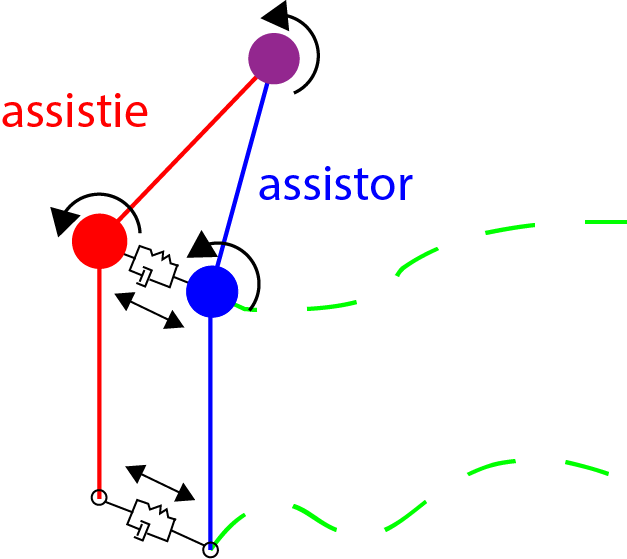
\includegraphics[scale=1.5]{images/controllers/double_pend.png}
    \caption[Double connected pendulum]{Double connected pendulum. Spring-dampeners connect the two pendulum (\textit{assistor} and \textit{assistie}) }
    \label{fig:double_pend}
\end{figure}

\begin{figure}
    \centering
    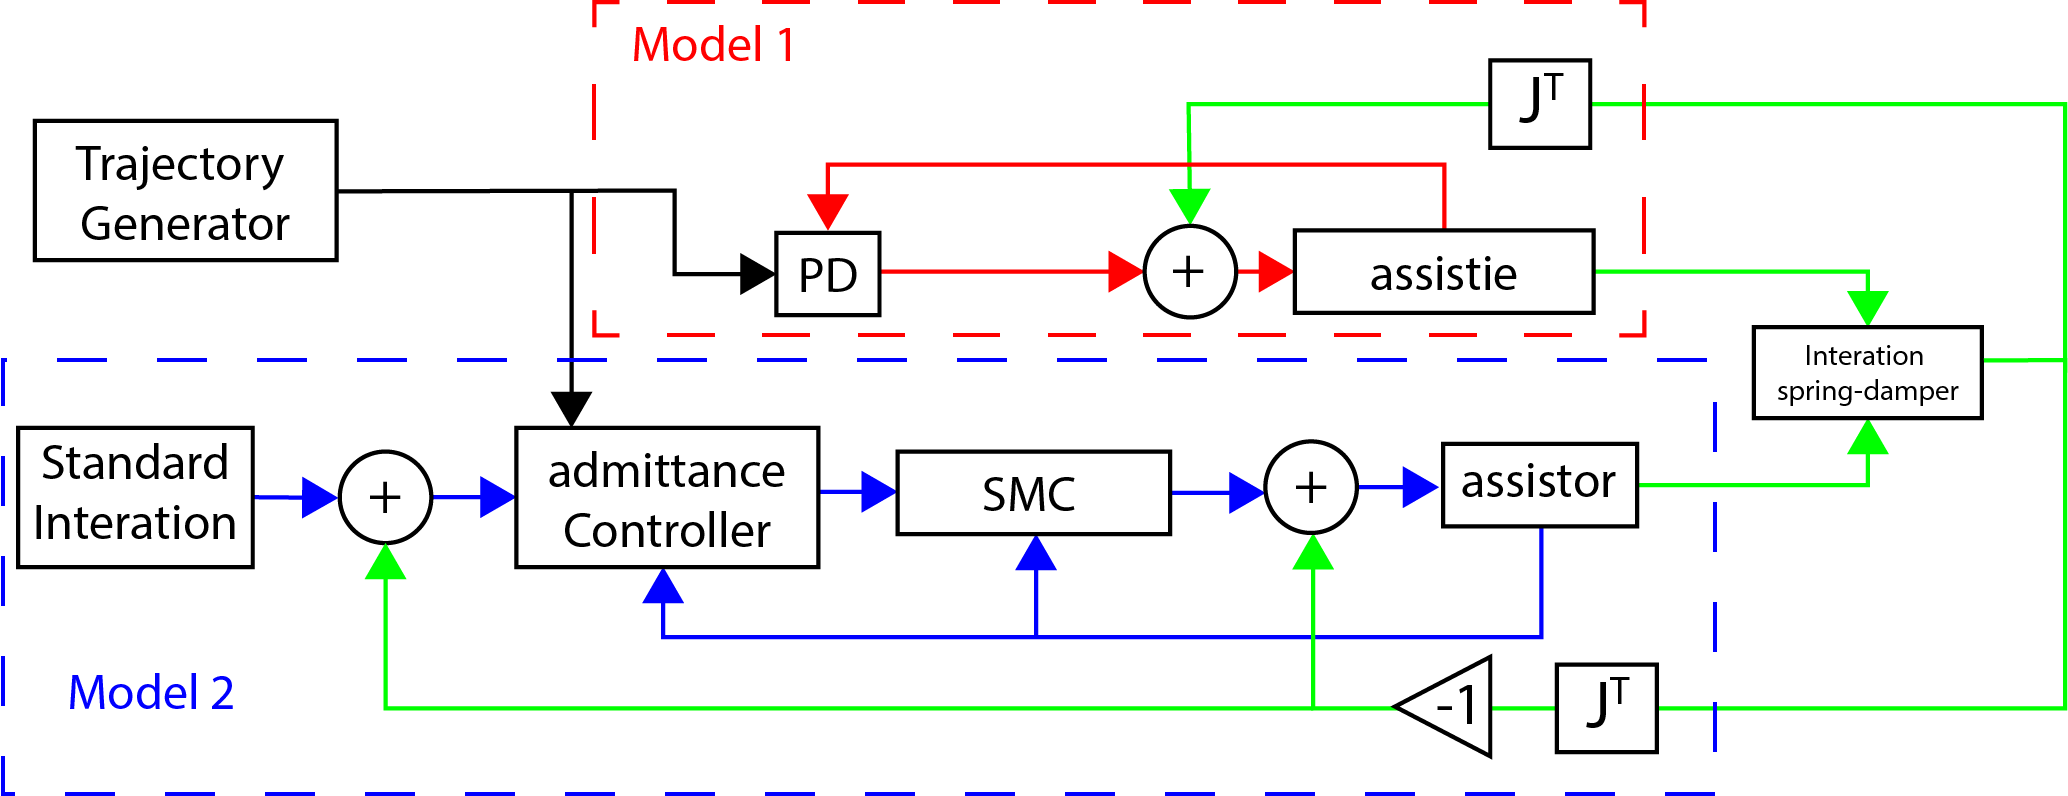
\includegraphics[width=\linewidth]{images/controllers/SMC_control_diagram_overview.png}
    \caption[Control diagram for A-SMC]{Control diagram for A-SMC}
    \label{fig:controlDiagram}
\end{figure}

\autoref{eq:CooPdyn} describes the dynamics for the \textit{assistor} (abbreviated has \textit{tor}) and \textit{assistie} (abbreviated has \textit{tie}) respectively.  It should be noted that $q$ is the joint state for the respective model that they describe. The $F$ terms are the forces generated as a result of being coupled by a spring dampener described by \autoref{eq:coupling}. Additionally, $J$ is the Jacobian of each link to the connection point of the spring dampener system. Although any point on the link could be used to calculate the Jacobian matrix, the connection point is at the end of each link. This assumption does change the process, only the calculation of the Jacobian matrix. It can later be adjusted to the location of the straps of the exoskeleton.

\begin{equation} 
\begin{aligned}
    M_{tor}(q) \ddot{q} + C_{tor} (q,\dot{q}) + G_{tor}(q) &= \tau_{tor} - J_{tor}^T F \\
    M_{tie}(q) \ddot{q} + C_{tie} (q,\dot{q}) + G_{tie}(q) &= \tau_{tie} + J_{tie}^T F
\end{aligned}
    \label{eq:CooPdyn}
\end{equation}

\begin{equation}
    F = K ( \vec{x}_{tor} - \vec{x}_{tie} ) + B (\dot{ \vec{x}}_{tor} - \dot{ \vec{x}}_{tie} ) 
    \label{eq:coupling}
\end{equation}


The \textit{assisitie} system was controlled by \autoref{eq:PDcnrl}. This is simple PD control framework. $K_p$ and $K_d$ are gain matrixs and $\vec{q}_d$ is the desired position. This torque however was capped to not exceed an absolute max torque value. This was accomplished using the following method, $| \vec{\tau}_{tie}|> \vec{\tau}_{max} \rightarrow \vec{\tau}_{tie} = sign(\vec{\tau}_{tie})*\vec{\tau}_{max}$.  This did not allow the controller to generate the required torque. 

\begin{equation}
        \tau_{tie} = K_p( \vec{q}_d - \vec{q}_{tie} ) + K_d ( \dot{\vec{q}}_d - \dot{\vec{q}}_{tie} ) 
    \label{eq:PDcnrl}
\end{equation}

The admittance controls the virtual dynamics of the system and how the systems interact \cite{faulring2005haptic}. If the \textit{assastie} system is capable of following the desired motion, the \textit{assasitor} system will be less aggressive. This interaction is controlled by \autoref{eq:addmittance}, where $x_a$ is the location of the virtual system and $x_d$ is the location of the point on the pendulum link. A separate spring-dampener system is on each of the links of the system. The virtual system is defined by the following terms $M_d$, $B_d$, and $K_d$ are inertia, dampening, and stiffness, respectively. As previously stated, it is desirable to have these parameters adjust on the fly to the intention and ability of the \textit{assistie} system. The variability is controlled by \autoref{eq:intention} and \autoref{eq:varible}. Here $\gamma_{n,p}$ and $\alpha_{n,p}$ are tuning variables for the damping and stiffness of the admittance controller. The admittance will control how quickly and aggressively the \textit{assistor} system will respond. If the stiffness or dampening is too large, the model will not track the desired motion.   

\begin{equation}
    \begin{aligned}
        \tau_{int} &= M_d^{-1}( K_d e_a + B_d \dot{e}_a)  \\
        e_a &= x_a - x_d 
    \end{aligned}
    \label{eq:addmittance}
\end{equation}

\begin{equation}
    \begin{aligned}
         intent &= bool ( sign(T_h) == sign(\dot{q}_d) ) \\
         \mu &= \Big|\frac{T_h}{T_{id}} \Big|
    \end{aligned}
    \label{eq:intention}
\end{equation}



\begin{equation}
    \begin{bmatrix} K_d \\ B_d \end{bmatrix} = \begin{cases}
        \begin{bmatrix} K_{p} \\ B_{p} \end{bmatrix} + \mu  \begin{bmatrix} \alpha_p  \\ \gamma_p \end{bmatrix}, intent = 1 \\
        \begin{bmatrix} K_{n} \\ B_{n} \end{bmatrix} - \mu  \begin{bmatrix} \alpha_n  \\ \gamma_n \end{bmatrix}, intent = 0
  \end{cases}
  \label{eq:varible}
\end{equation}


The A-SMC controller suffers from an abundance of tunable parameters. The admittance controller and SMC have parameters requiring synergistic tuning since these systems are connected.  A gradient descent method is used to find optimal parameters based on various cost functions and constraints for the controller.  Gradient descent is used since it should arrive quickly to a solution  \cite{piltan2012performance} \cite{wang1996course}. The goal is to minimize the objective function by updating parameters. This method will iterate until the objective function converges to a locally optimal location. The tunable parameters for this controller are the variable admittance parameters ($K_{n,p}$, $B_{n,p}$, $\alpha_{n,p}$, $\gamma_{n,p}$) and the sliding mode controller variables ($\rho$, $\Lambda$, $\beta$).  Another important variable is the limit of the torque that the \textit{assistor} system can provide, and this limitation is important since real physical systems cannot produce infinite torque. Motors and gearboxes present real limitations on the system. This method allows for the maximum torque to be used, has a hard limitation, and allows for the minimal limit to be found.


The optimization was calculated using Simulink Response Optimization\footnote{https://www.mathworks.com/help/sldo/response-optimization.html}. Several cost functions were tested to find the optimal performance, and the model was trained to follow a polynomial trajectory. Root mean squared error (RMSE) was used for the cost function shown in \autoref{eq:RMSE}, where $x$ is the observation and $\hat{x}$ is the reference, either position or velocity. The error is summed along both the trajectory and the joints to get a scalar value. If both the position and velocity RMSE are used, it is summed.

The gain parameters $K_p$ and $K_d$ in \autoref{eq:PDcnrl} were also tuned using the same method. The controller assumed that no assistance was provided by the \textit{assistor} system. These gains were set for the \textit{assistie} controller in the closed-loop system.

\begin{equation}
    e = \sqrt{ \frac{ \sum_1^N ( \hat{x}_i - x_i )^2 }{N}  }
    \label{eq:RMSE}
\end{equation}

\subsubsection{Tuning of Cooperative Controller}
Several different cost functions were tested to arrive at a cost function for parameter tuning. It was assumed that the \textit{assistie} system. Three different cost functions were tested, one based on position, another on velocity, and finally, one used both position and velocity.


\autoref{fig:cost_function_optimization} shows the conversions of the cost functions used for optimization. All the cost functions converged to a steady value after approximately ten iterations; this means that the tuned controllers' parameters reached a local point where the system's performance was steady as defined by the cost. This is not a direct correlation to the actual system performance. By examining the system's state space, the performance of the controller can be a better detriment.





\begin{figure}[ht]
    \begin{subfigure}{0.5\textwidth}
        \centering
        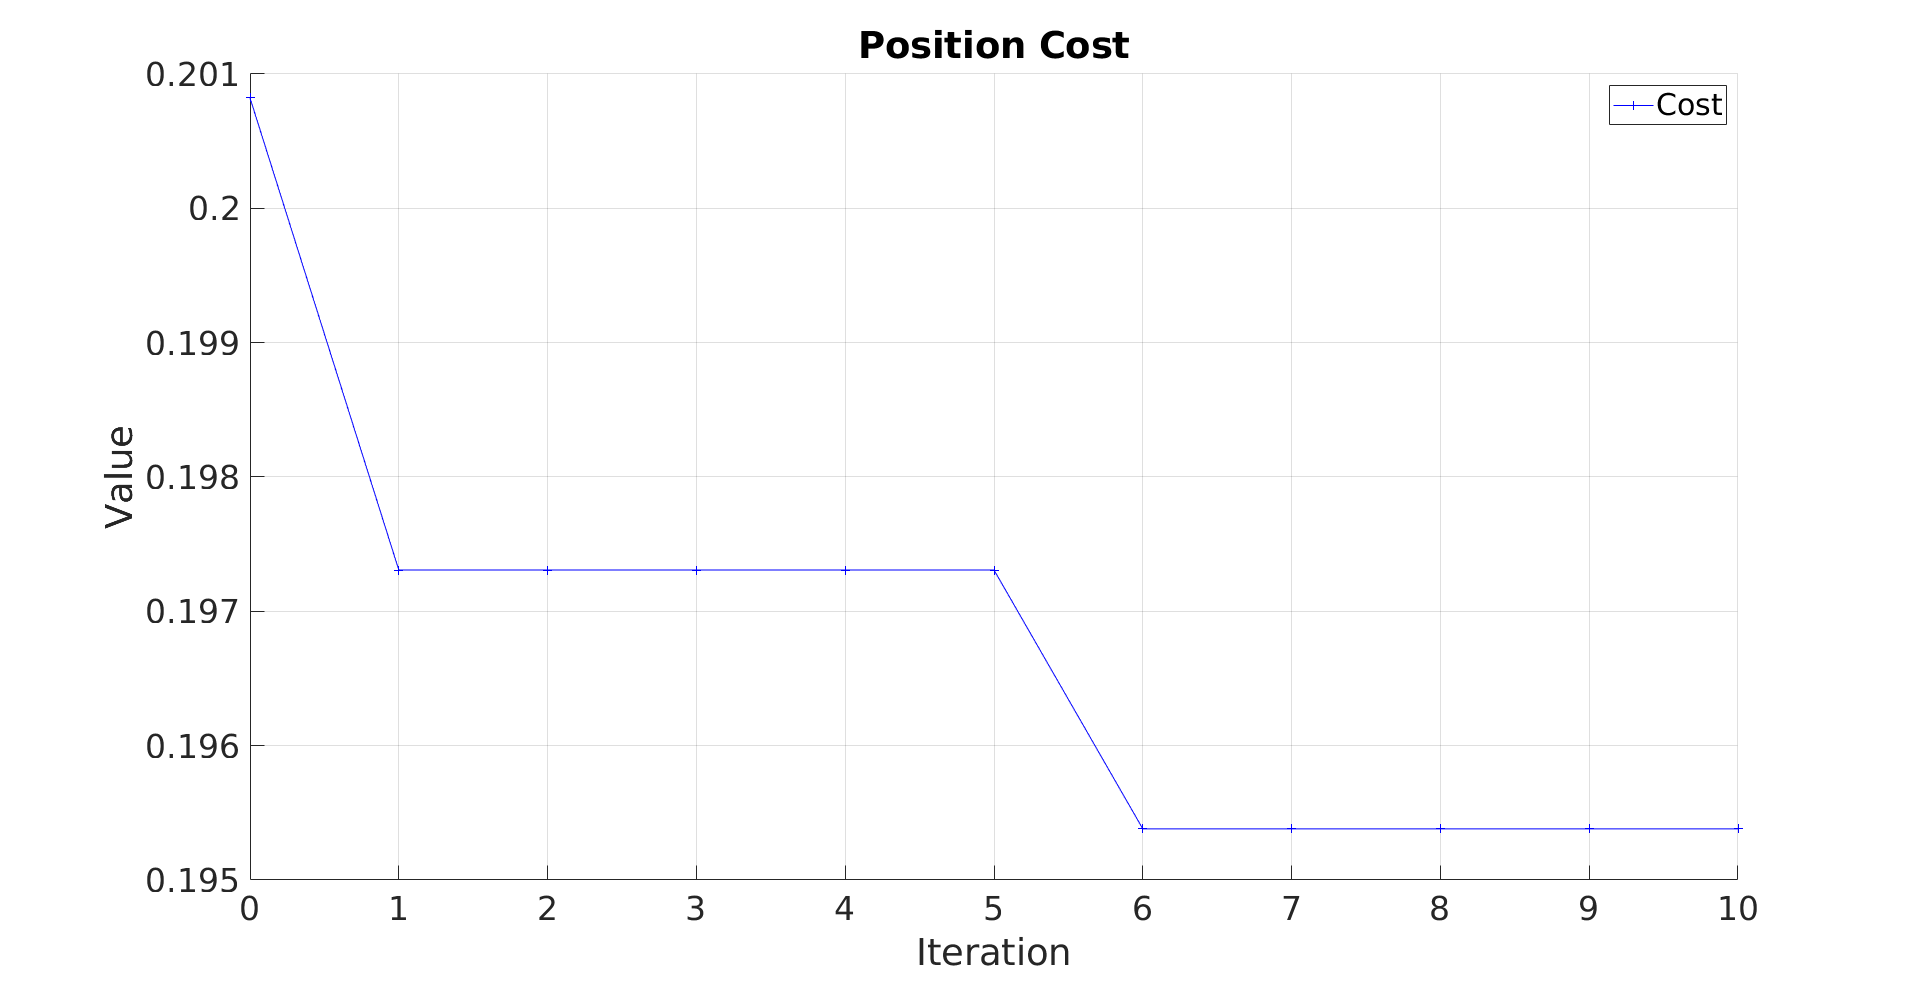
\includegraphics[width=0.9\linewidth]{images/controllers/pos_cost.png}
        \caption[Position cost function]{Convergence of position cost function}
        \label{fig:pos_cost}
    \end{subfigure}
    \begin{subfigure}{0.5\textwidth}
        \centering
        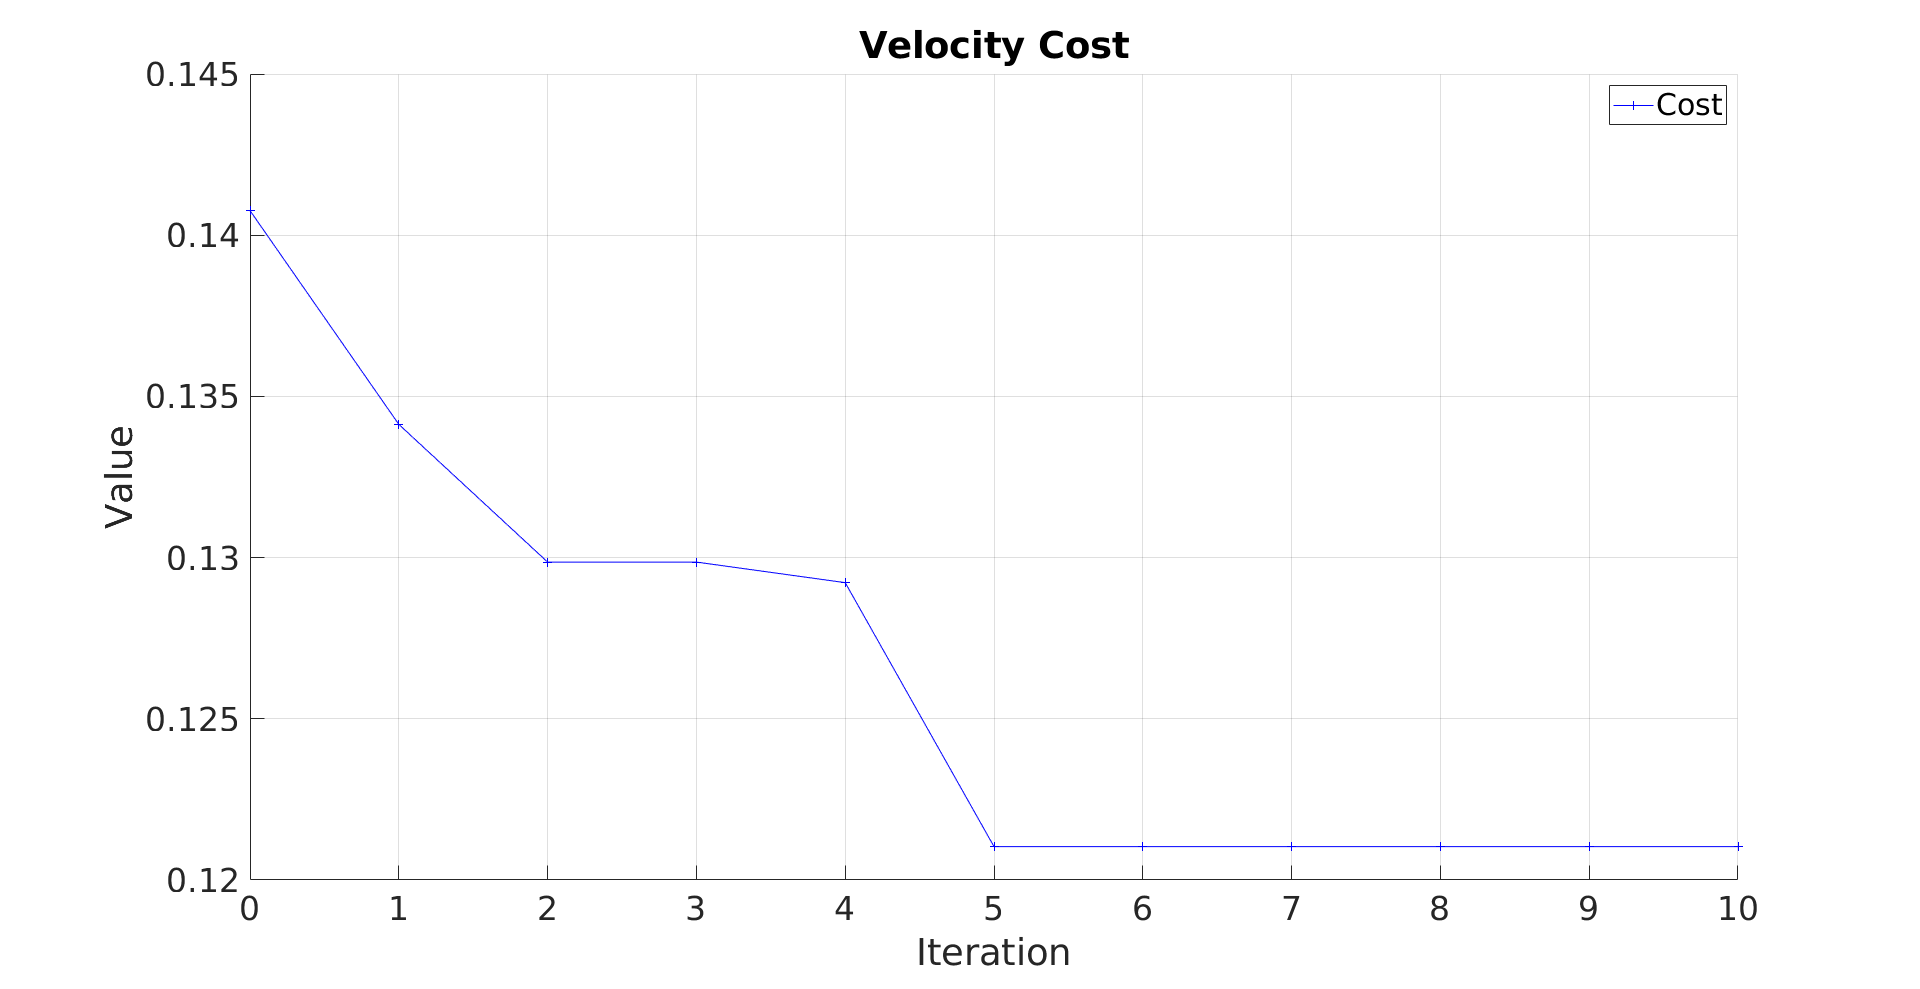
\includegraphics[width=0.9\linewidth]{images/controllers/vel_cost.png}
        \caption[Velocity cost function]{Convergence of velocity cost function}
        \label{fig:vel_cost}
    \end{subfigure}

    \begin{subfigure}{\textwidth}
        \centering
        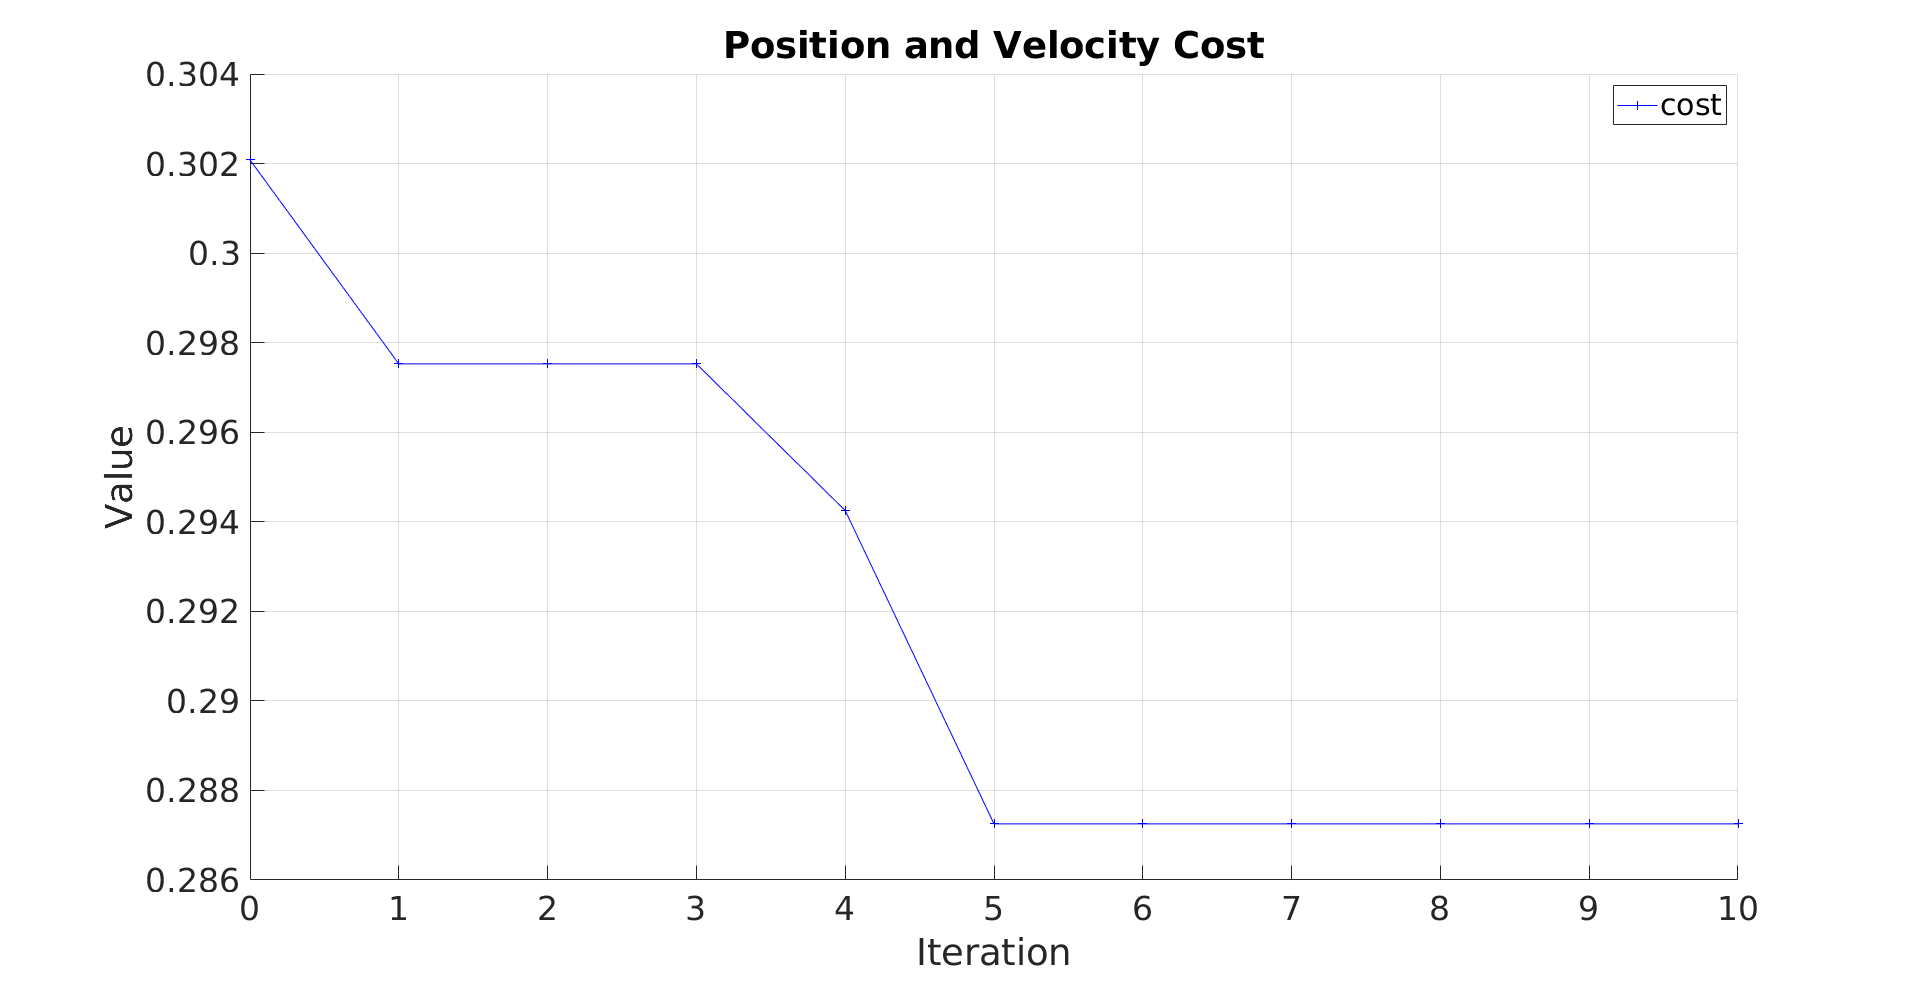
\includegraphics[width=0.45\linewidth]{images/controllers/all_cost.png}
        \caption[Combined cost function]{Convergence of combined cost function}
        \label{fig:all_cost}
    \end{subfigure}
    \caption{Cost function convergence for the different cost functions}
    \label{fig:cost_function_optimization}
\end{figure}


The state-space of the system response is shown in  \autoref{fig:statespace}. The output of each of the tuning methods was compared throughout this paper. The untuned gains are also shown for reference to show the improvement of the output. The response optimizer was tuned until the cost function converged. The untuned gains performed poorly and were able to reach the settling point. Using the position tuning caused a significant spike in the sliding surface for both joints. Using position and velocity had similar results as just using velocity to the cost function. 


\begin{figure}[ht!]
    \centering
    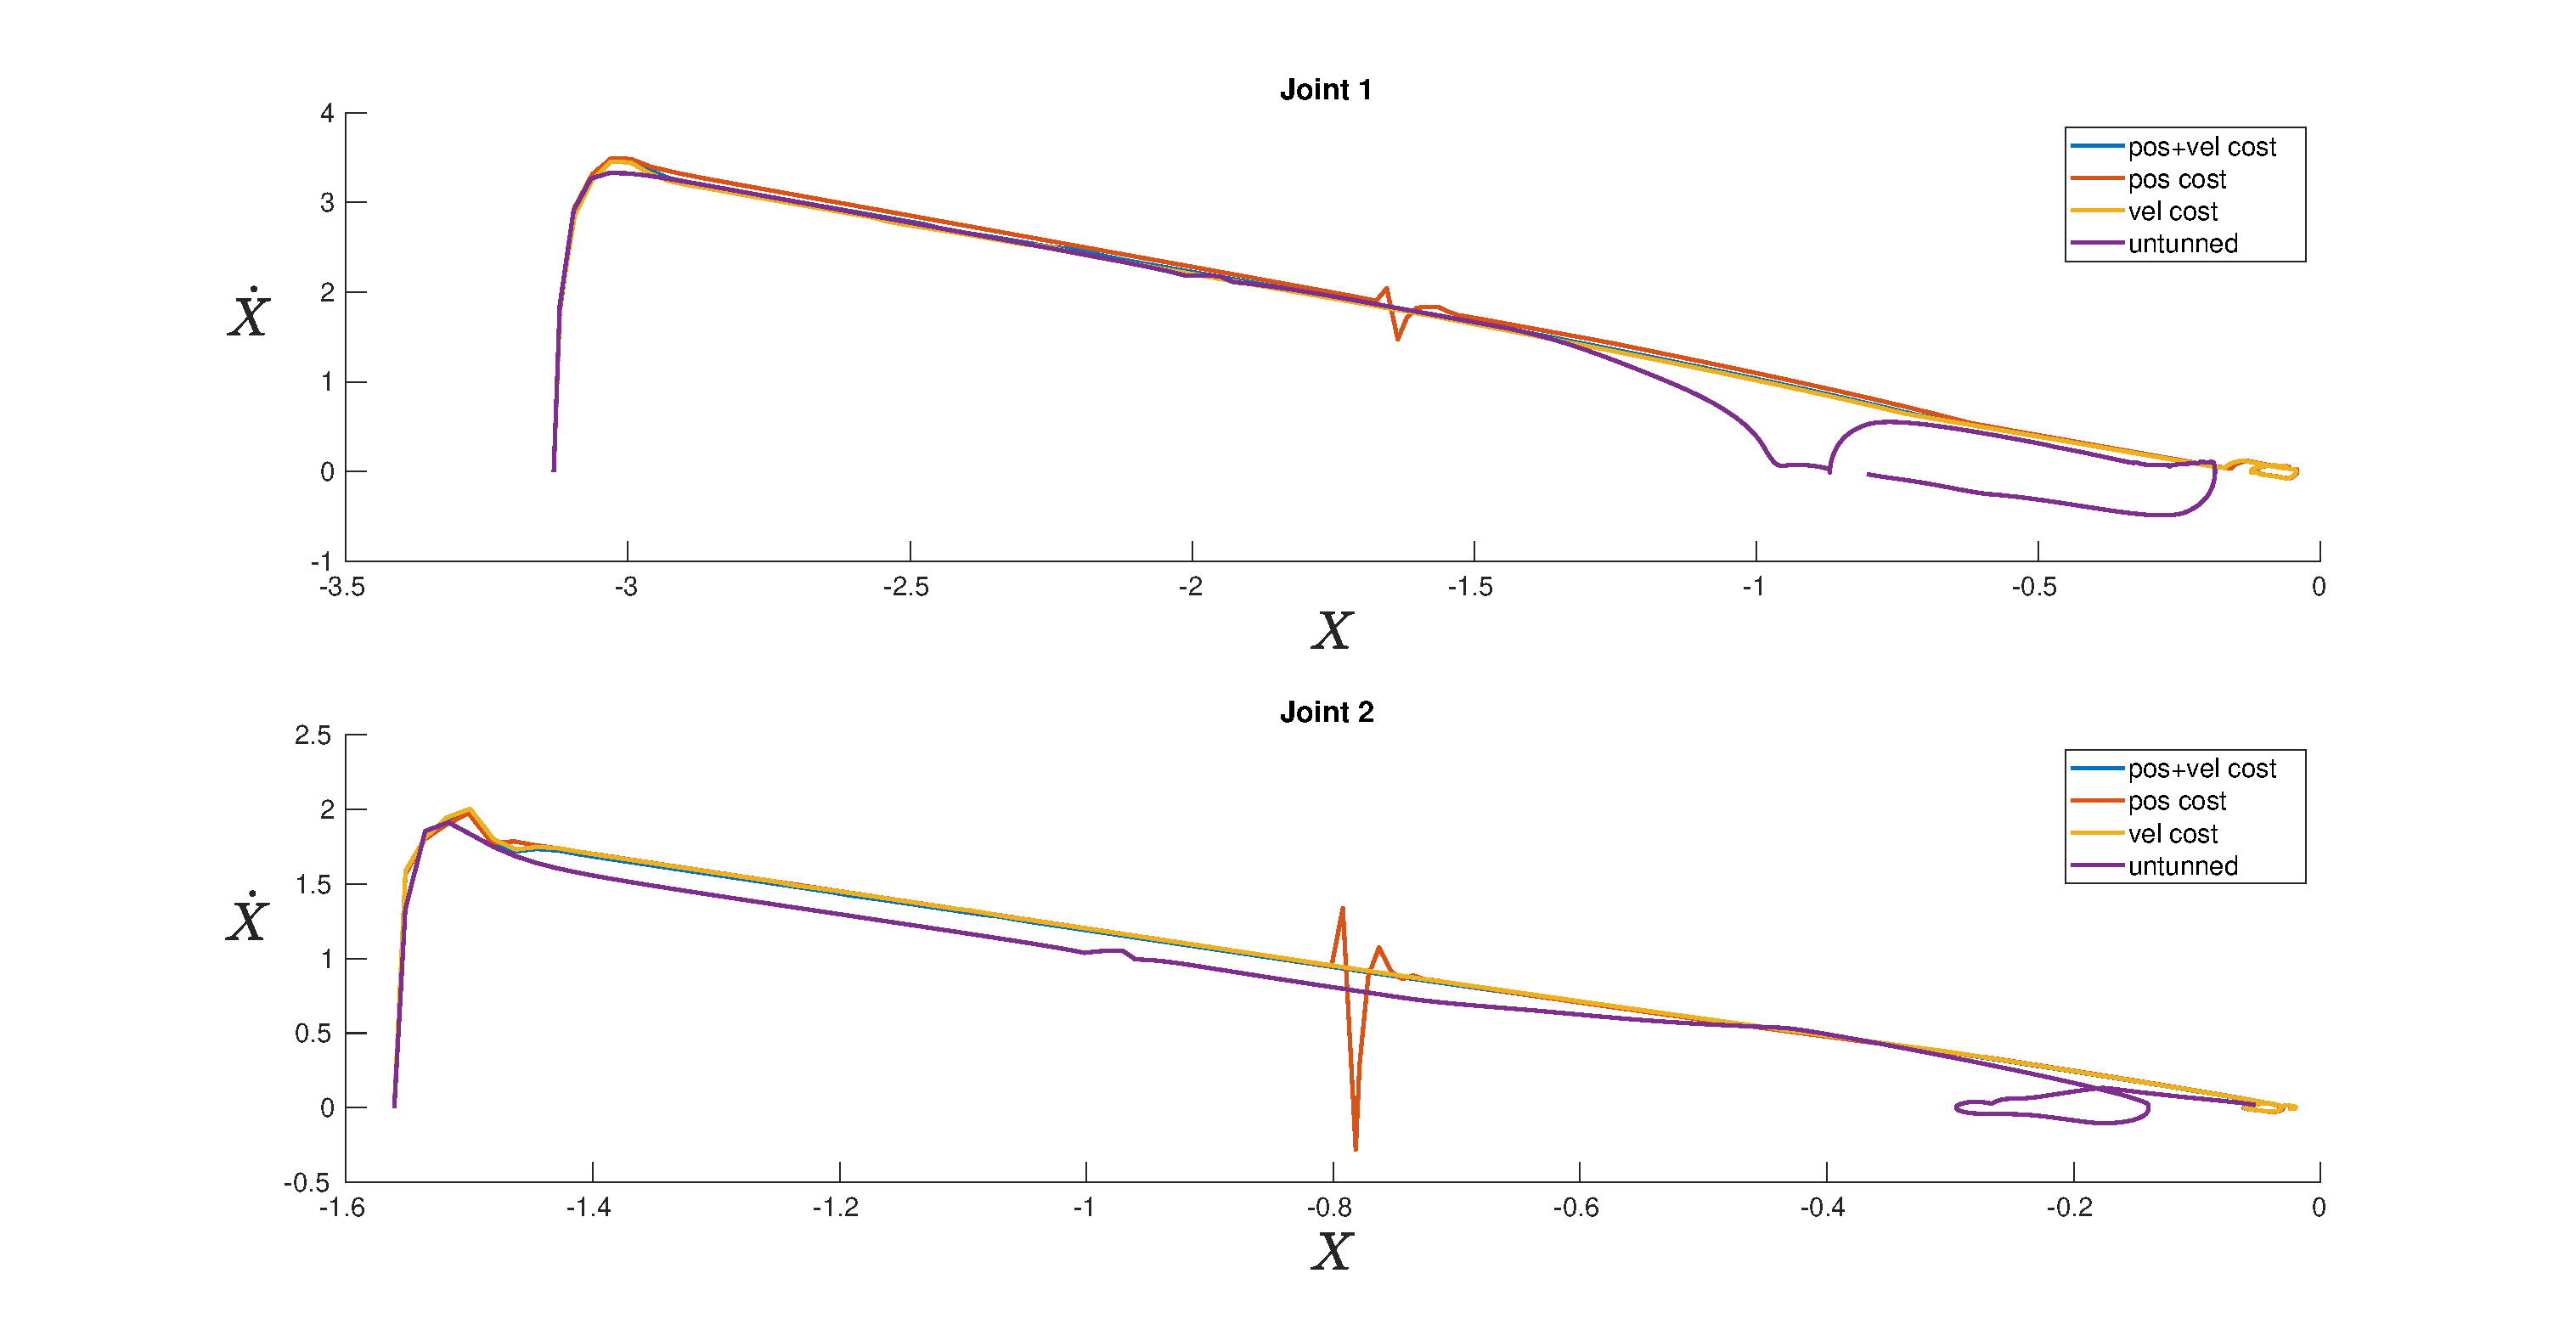
\includegraphics[width=\linewidth]{images/controllers/statespace.eps}
    \caption[A-SMC State Space]{Comparing different cost functions used to tune the A-SMC controller}
    \label{fig:statespace}
\end{figure}

Different involvement of the \textit{assistie}  using the tuned gains, reduced involvement, time-varying, and no involvement were tested. Additional varying alignment methods were tested to show the effect of the systems not being perfectly aligned with the length of the \textit{assistor}. The alignment methods included changing the links by $\pm 5\%$ of the \textit{assistie} link lengths. \autoref{fig:no_effort} shows the effects with no involvement from the \textit{assistie} system. All the effort is being supplied by the \textit{assistor} system's A-SMC. As shown \autoref{fig:no_effort_traj}, the controller was able to track the desired trajectory. 

\begin{figure*}[h!]
    \centering
    \begin{subfigure}{0.5\textwidth}
        \centering
        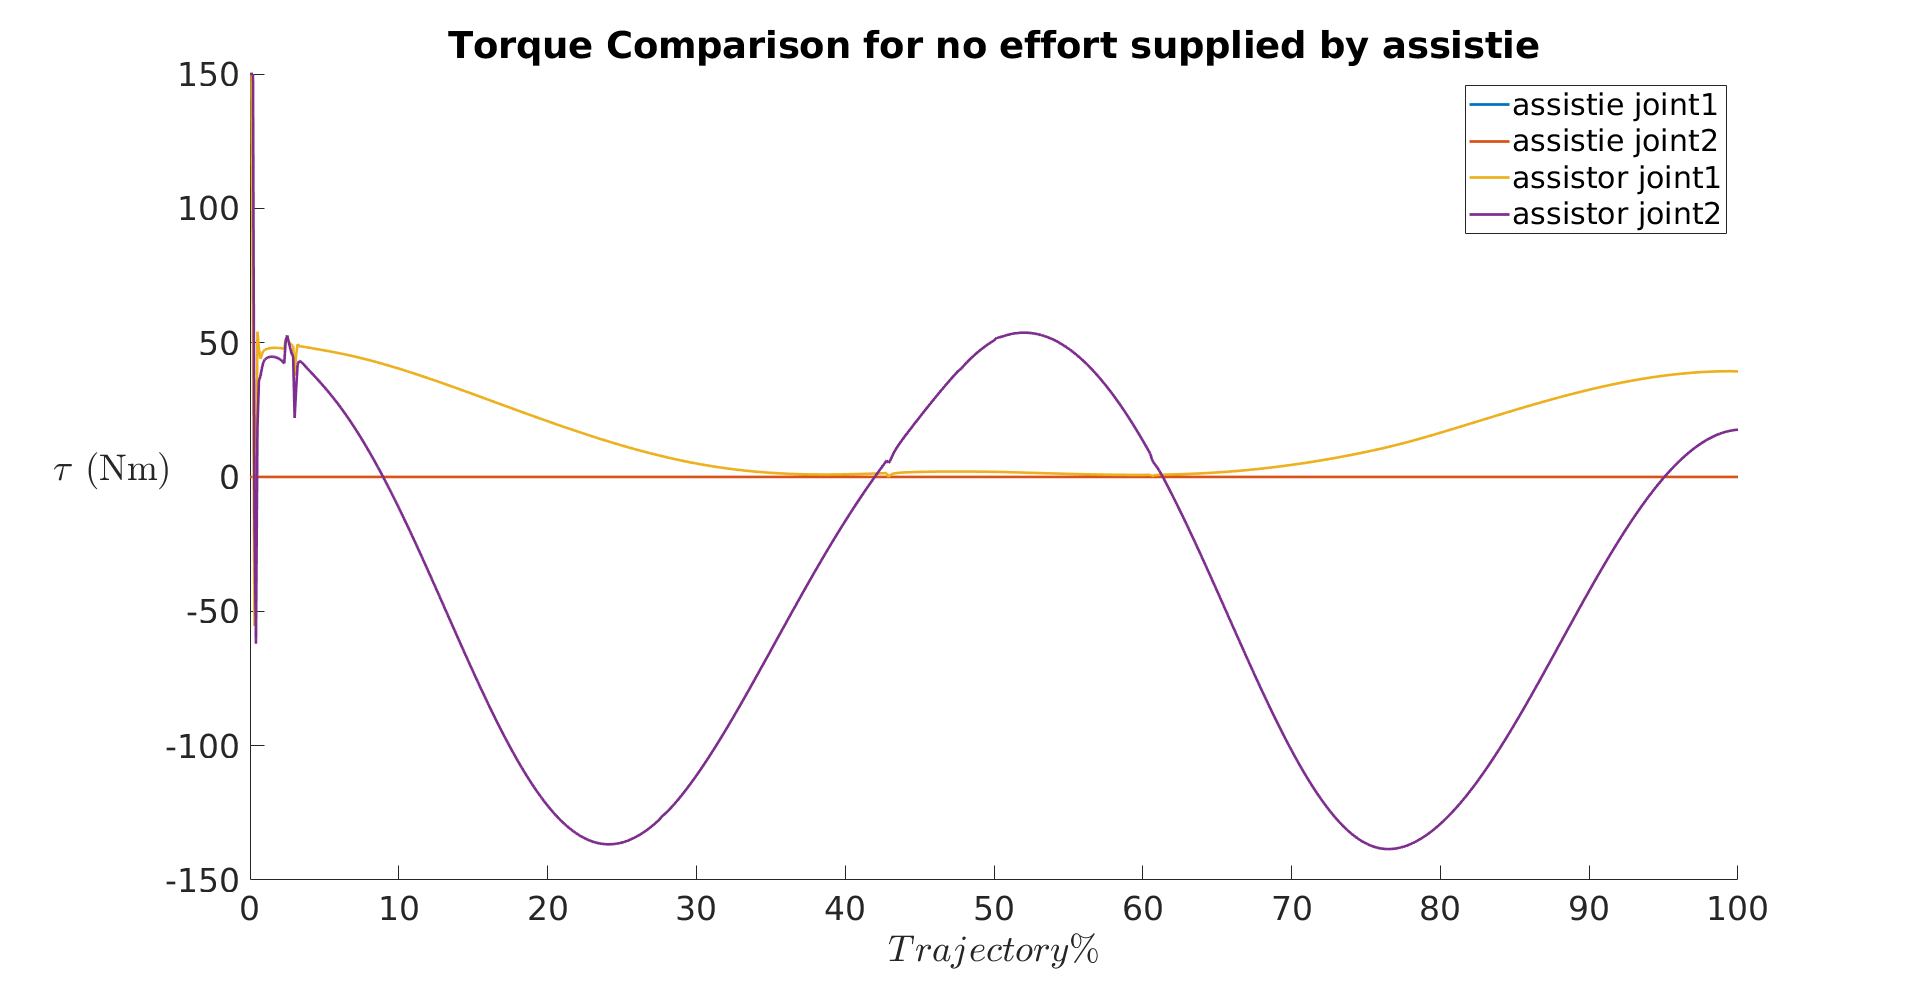
\includegraphics[width=\linewidth]{images/controllers/none_torque.png}
        \caption[Double Pendulum: No Torque-Effort]{Torque applied to the double pendulum}
        \label{fig:no_effort_torque}
    \end{subfigure}%
    ~
    \begin{subfigure}{0.5\textwidth}
        \centering
        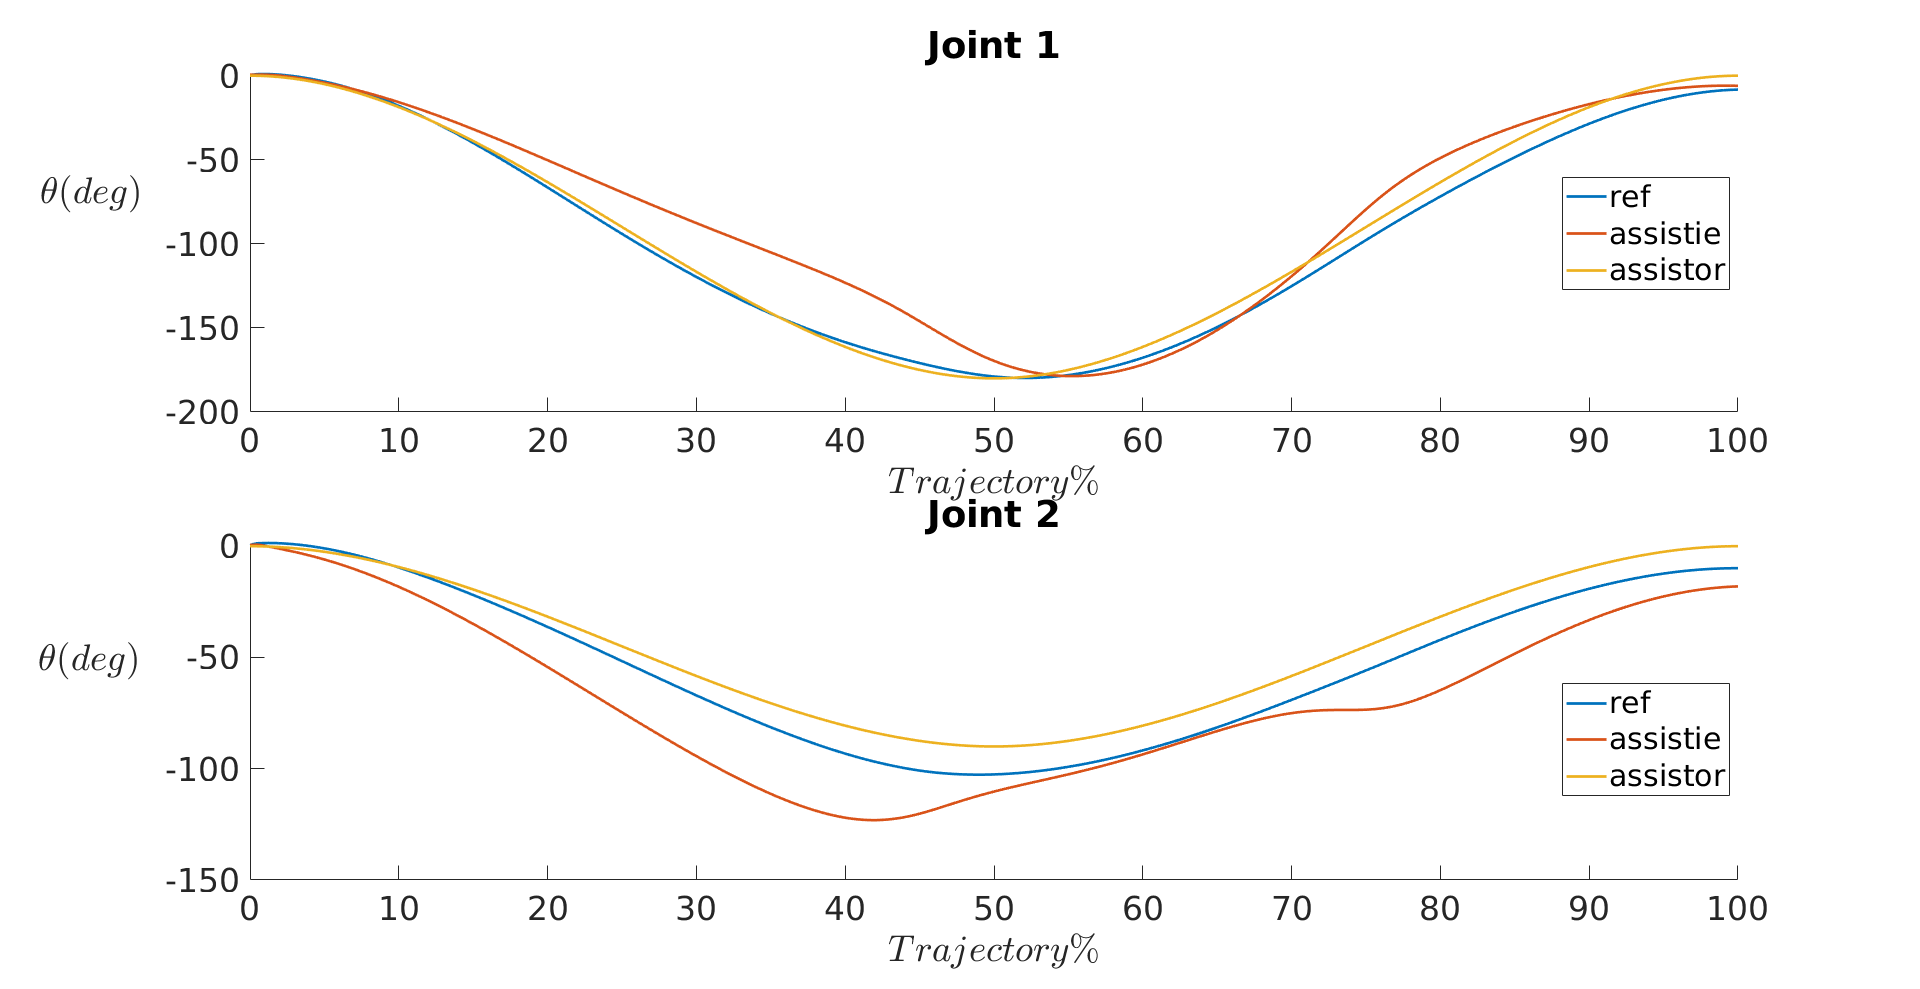
\includegraphics[width=\linewidth]{images/controllers/none_traj.png}
        \caption[Double Pendulum: No Torque-Trajectory]{Trajectories of double pendulum}
        \label{fig:no_effort_traj}
    \end{subfigure}
    \caption[Double Pendulum: No Torque]{Double pendulum model responses with no \textit{assistie} torques.}
    \label{fig:no_effort}
\end{figure*}

\autoref{fig:reduced_effort} shows the effects with a reduced involvement from the \textit{assistie} system. The \textit{assistie} system was only capable of producing approximately 20\%  of the required torque. The PD controller controlling the \textit{assistie} system worked together with the A-SMC controlling the \textit{assistor} to track the desired motions.

\begin{figure*}[h!]
    \centering
    \begin{subfigure}{0.5\textwidth}
        \centering
        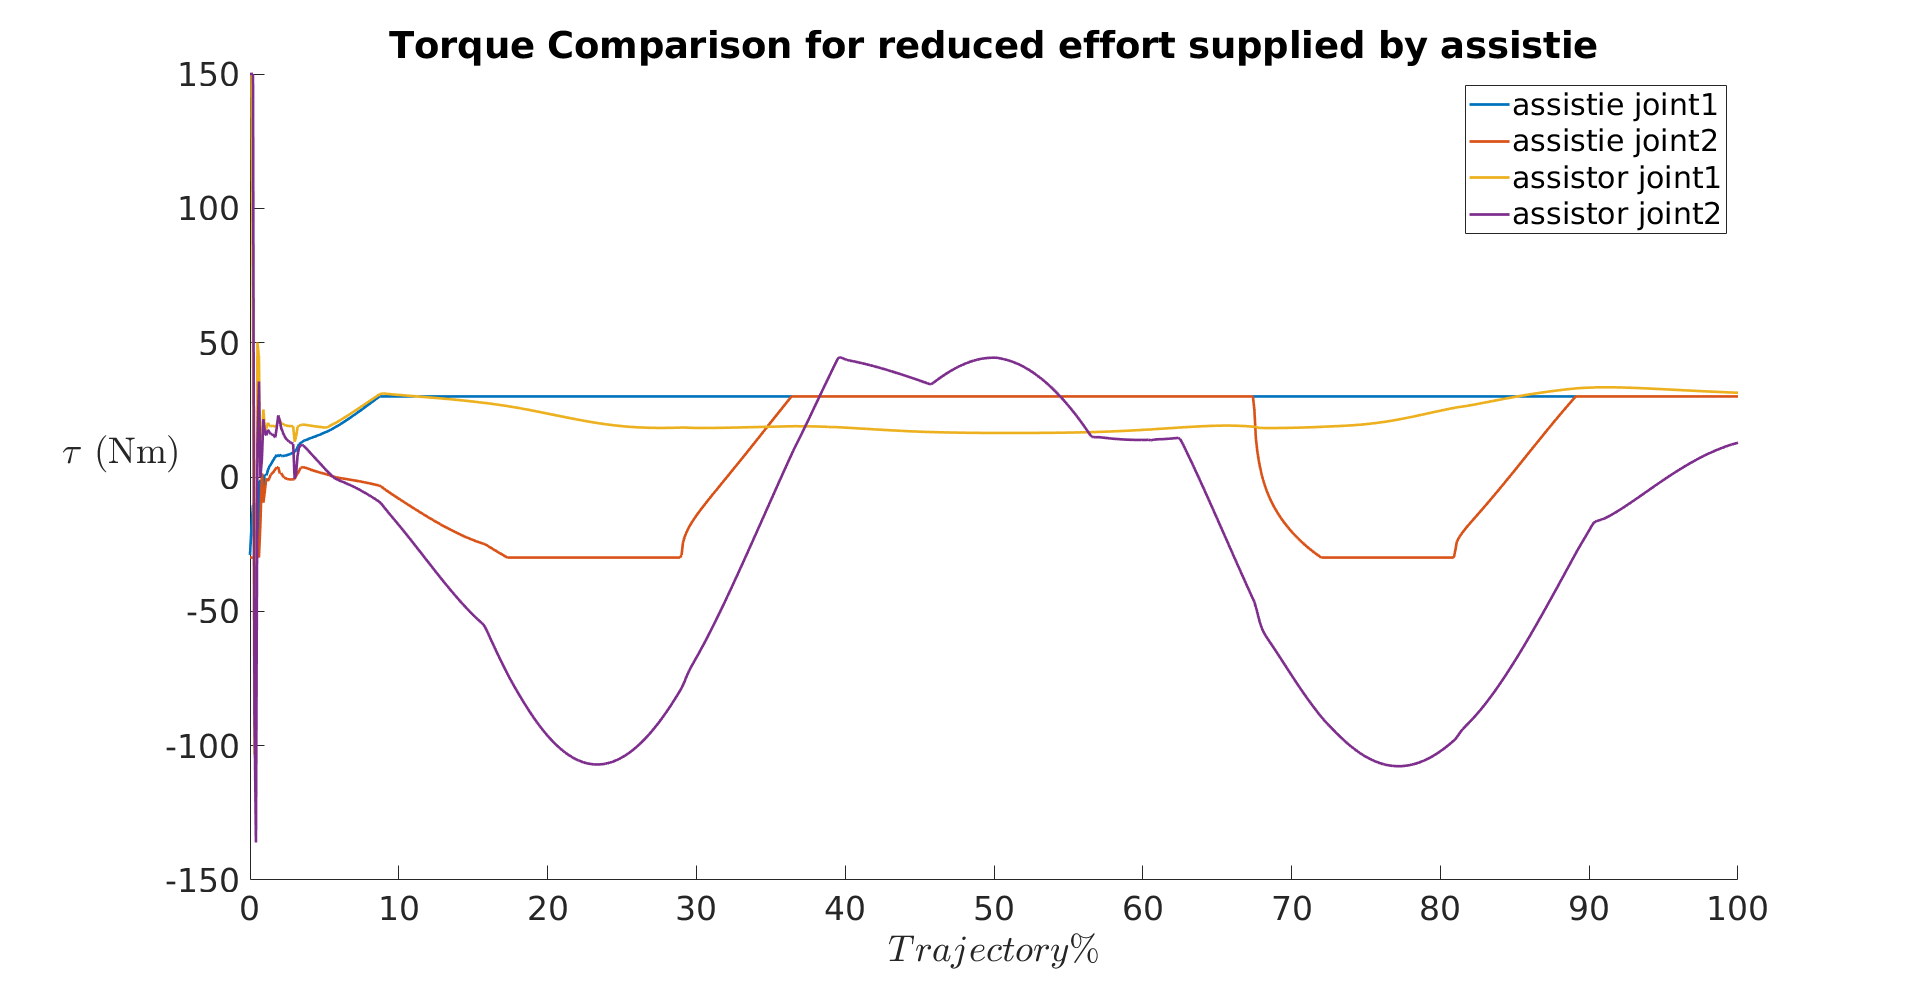
\includegraphics[width=\linewidth]{images/controllers/reduced_torque.png}
        \caption[Double Pendulum: Reduced Torque-Effort]{Torque applied to the double pendulum}
        \label{fig:reduced_effort_torque}
    \end{subfigure}%
    ~
    \begin{subfigure}{0.5\textwidth}
        \centering
        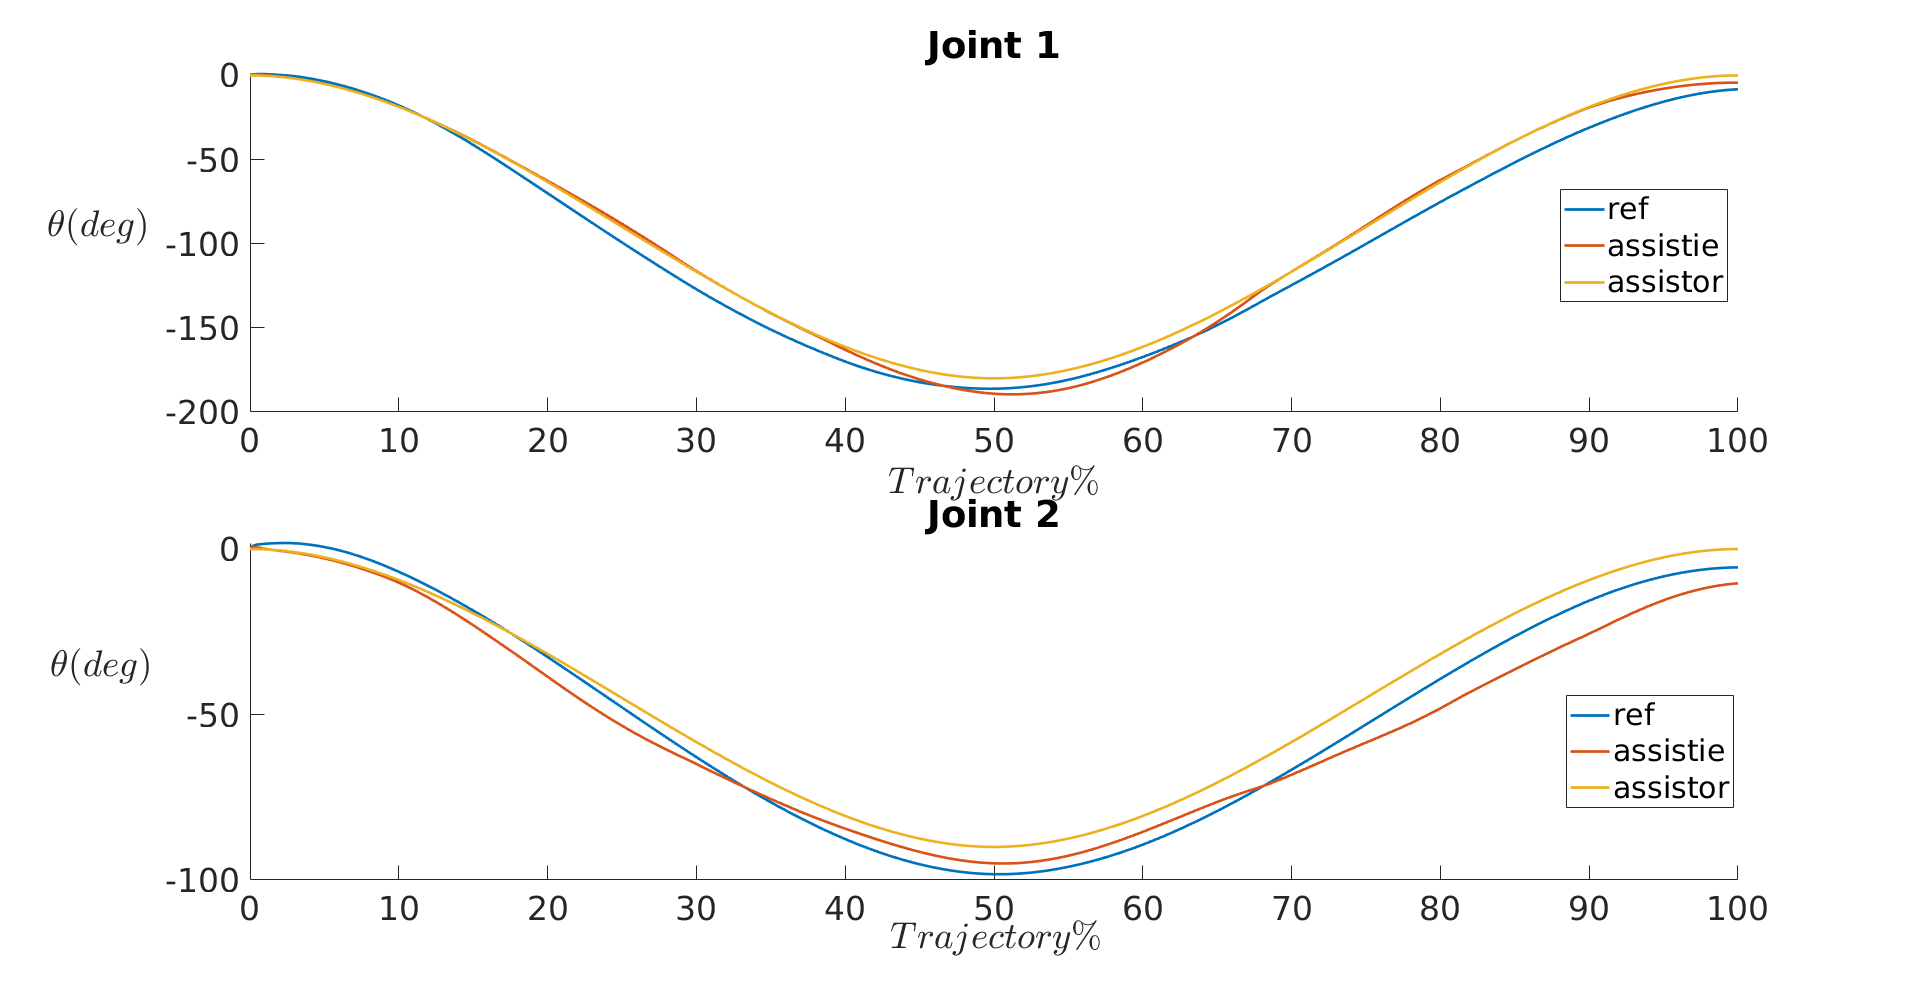
\includegraphics[width=\linewidth]{images/controllers/reduced_traj.png}
        \caption[Double Pendulum: Reduced Torque-Trajectory]{Trajectories of double pendulum}
        \label{fig:reduced_effort_traj}
    \end{subfigure}
    \caption[Double Pendulum: Reduced Torque]{Double pendulum model responses with reduced \textit{assistie} torques.}
    \label{fig:reduced_effort}
\end{figure*}

\autoref{fig:time_varying} shows the effects with a reduced involvement from the \textit{assistie} system. The \textit{assistie} system was only capable of producing approximately 20\%, and it was reduced over time by multiplying it $e^{-\xi t}sin(t)$; this was done to simulate a reduction in torque over time. The A-SMC controlling the \textit{assistor} had to handle the change in involvement over time. 

\begin{figure}[h]
    \centering
    \begin{subfigure}{0.5\textwidth}
        \centering
        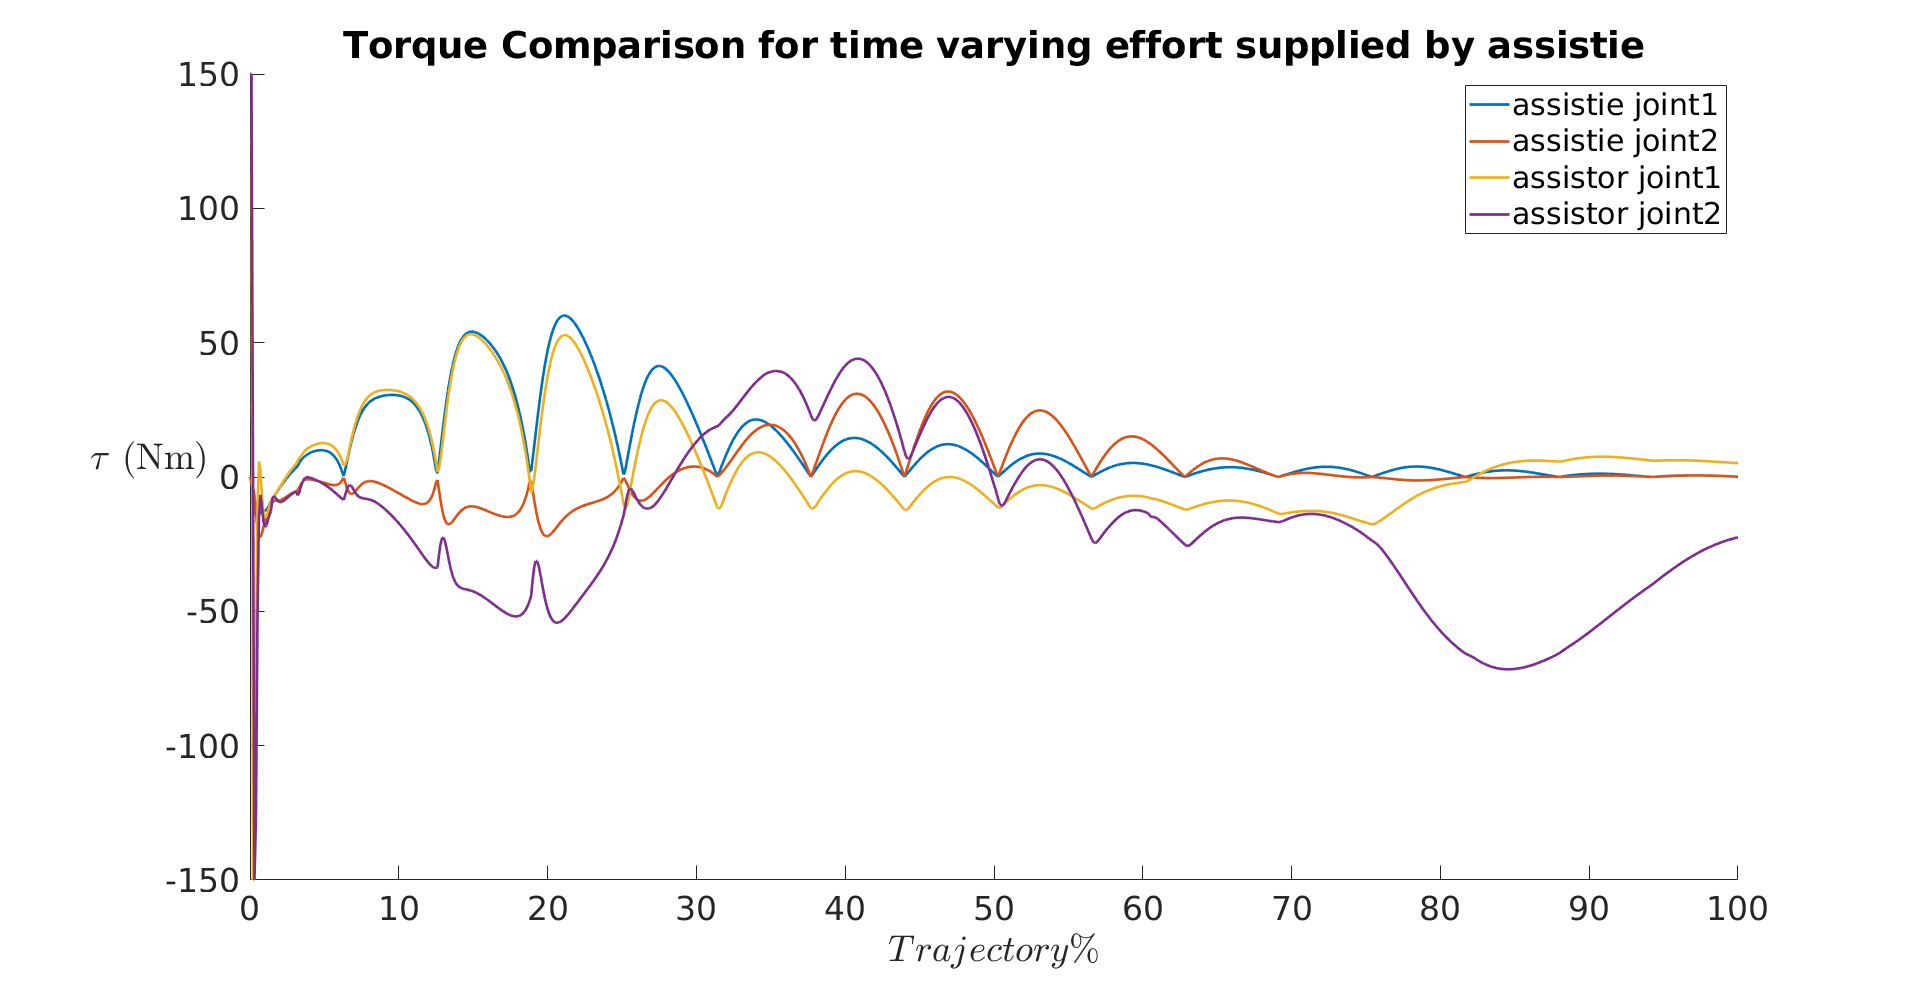
\includegraphics[width=\linewidth]{images/controllers/time_varying_torque.png}
        \caption[Double Pendulum: Time varying Torque-Effort]{Torque applied to the double pendulum}
        \label{fig:time_varying_torque}
    \end{subfigure}%
    ~
    \begin{subfigure}{0.5\textwidth}
        \centering
        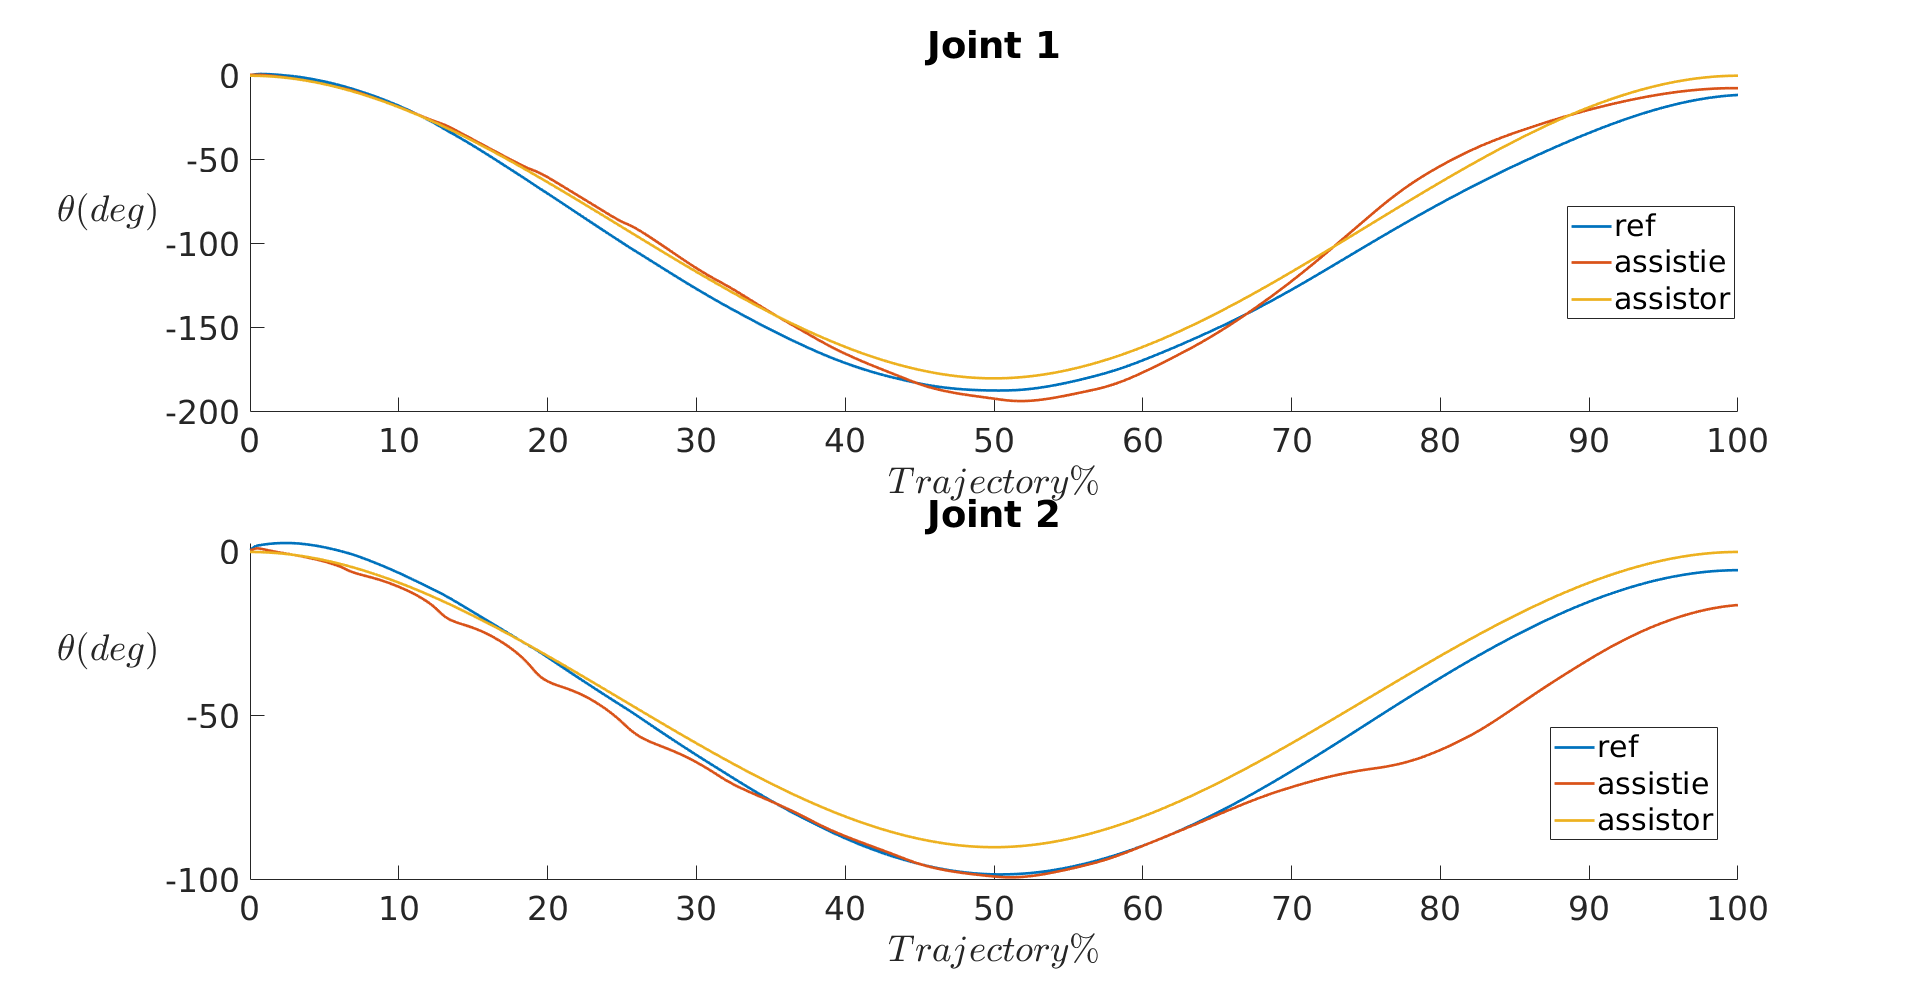
\includegraphics[width=\linewidth]{images/controllers/time_varying_traj.png}
        \caption[Double Pendulum: Time Varying Effort-Trajectory]{Trajectories of double pendulum}
        \label{fig:time_varying_traj}
    \end{subfigure}
    \caption[Double Pendulum: Time Varying Torque]{Double pendulum model responses with time varying reduced \textit{ assistie} torques.}
    \label{fig:time_varying}
\end{figure}


Additionally, the effects of the controller were tested with a misalignment between the \textit{assistie} and \textit{assistor} systems. The time-varying control signal was used for these tests. The length of the \textit{assistor} system was changed by $\pm 5\%$; this would simulate an exoskeleton that does not perfectly align with the person. The effects are shown in misalignment are shown in \autoref{fig:small_length} and \autoref{fig:larger_length}.

\begin{figure}[h!]
    \centering
    \begin{subfigure}{0.5\textwidth}
        \centering
        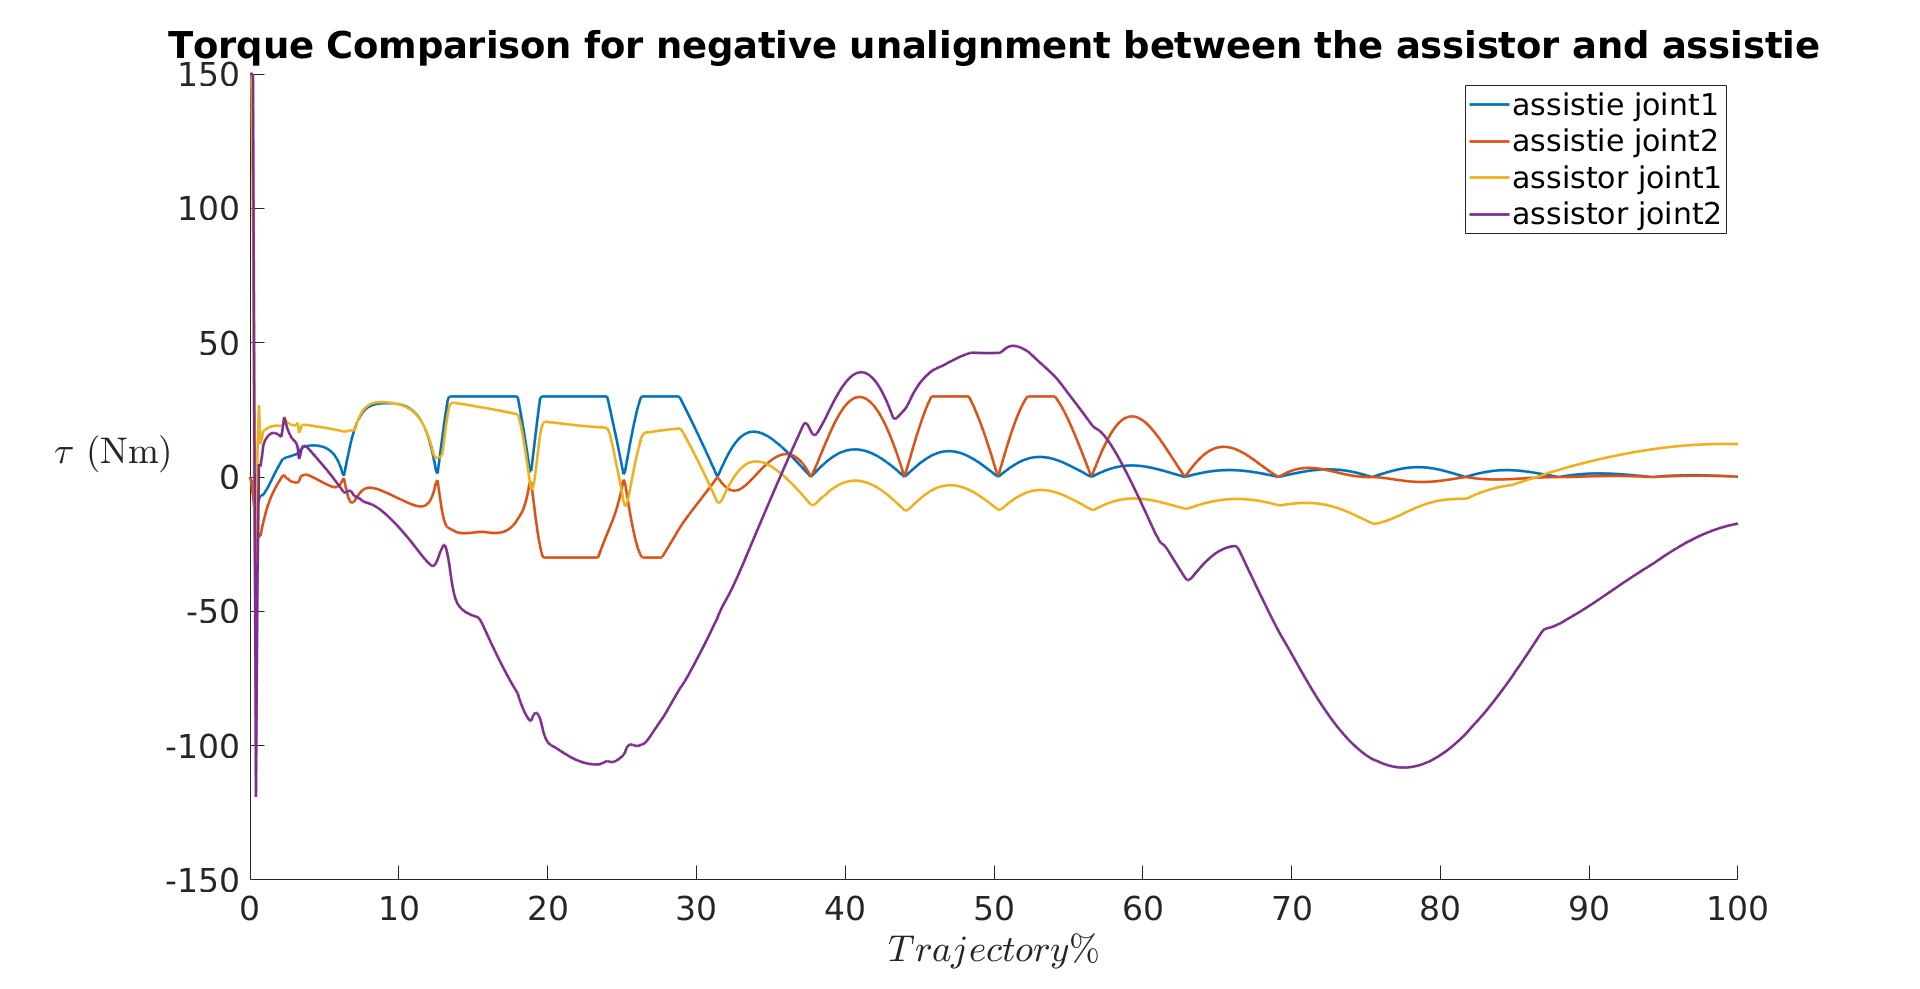
\includegraphics[width=\linewidth]{images/controllers/small_length_torque.png}
        \caption[Double Pendulum: Negative Alignment-Effort]{Torque applied to the double pendulum}
        \label{fig:small_length_torque}
    \end{subfigure}%
    ~
    \begin{subfigure}{0.5\textwidth}
        \centering
        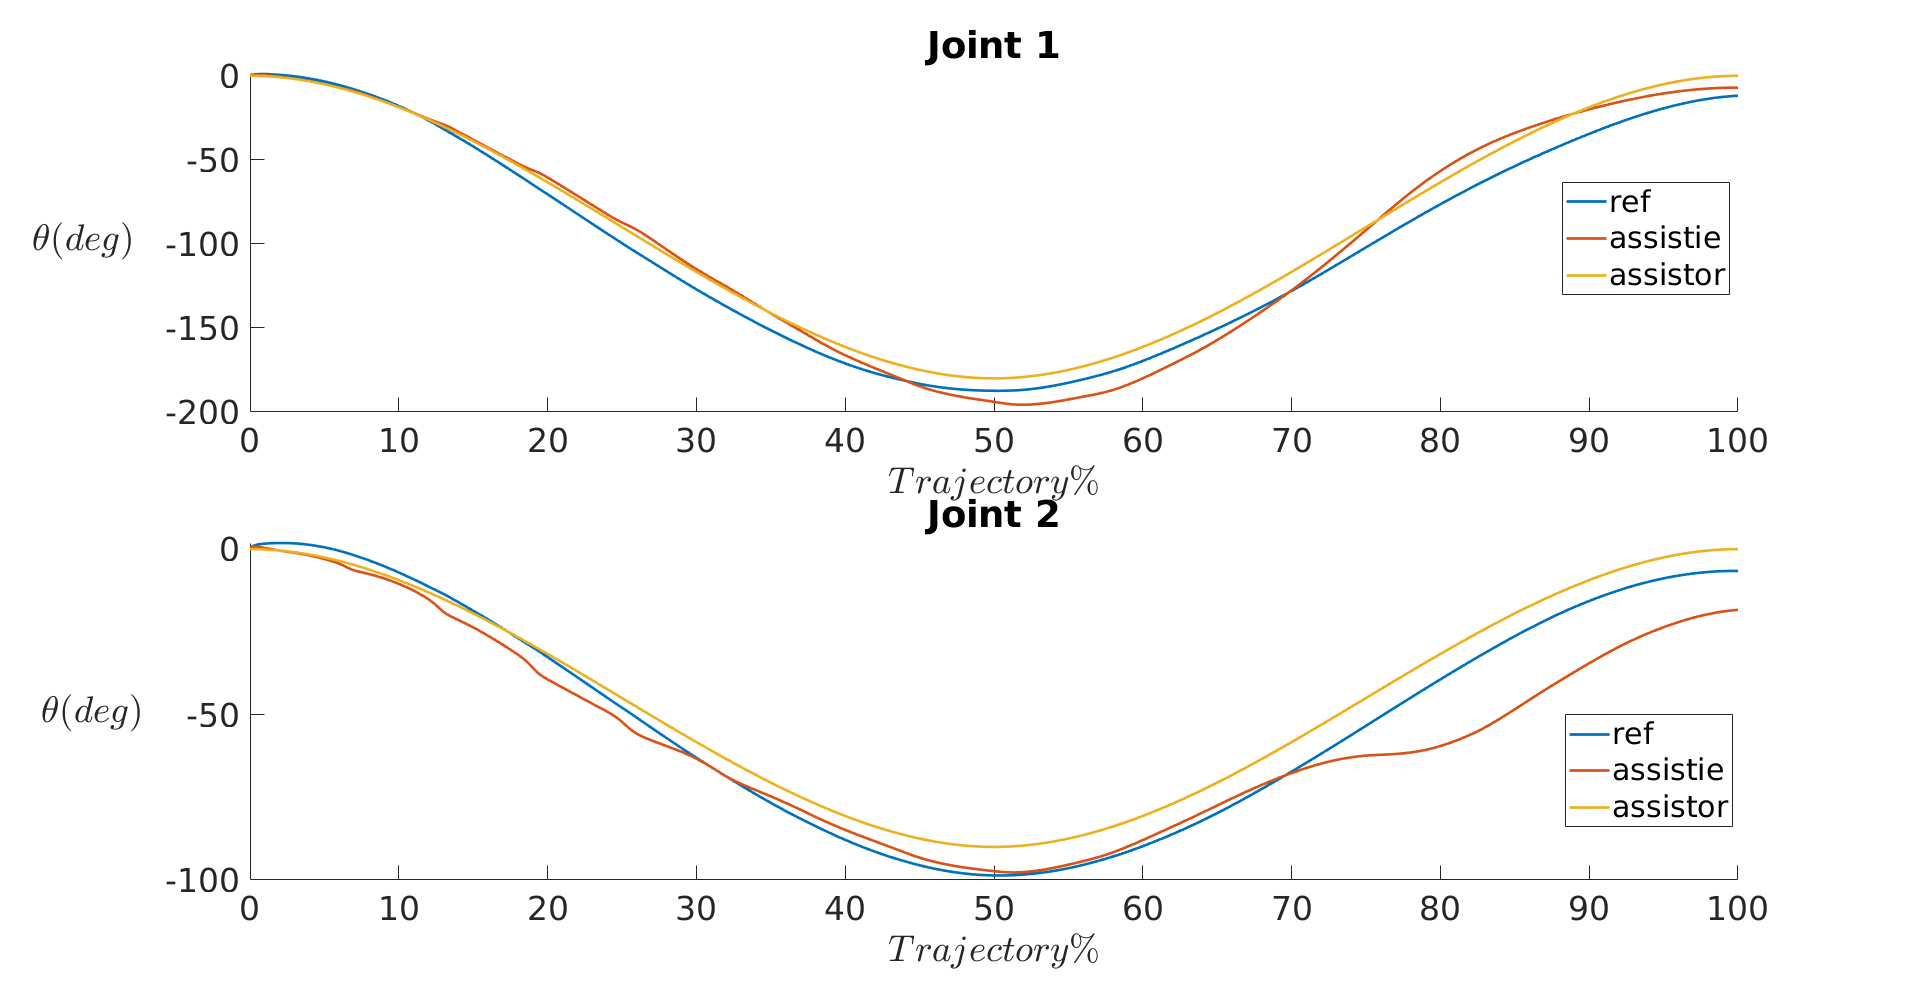
\includegraphics[width=\linewidth]{images/controllers/small_length_traj.png}
        \caption[Double Pendulum: Negative Alignment-Trajectory]{Trajectories of double pendulum}
        \label{fig:small_length_traj}
    \end{subfigure}
    \caption[Double Pendulum: Negative Alignment]{Double pendulum model responses with at 0.95x of the human length \textit{assistie} torques.}
    \label{fig:small_length}
\end{figure}

\begin{figure}[h]
    \centering
    \begin{subfigure}{0.5\textwidth}
        \centering
        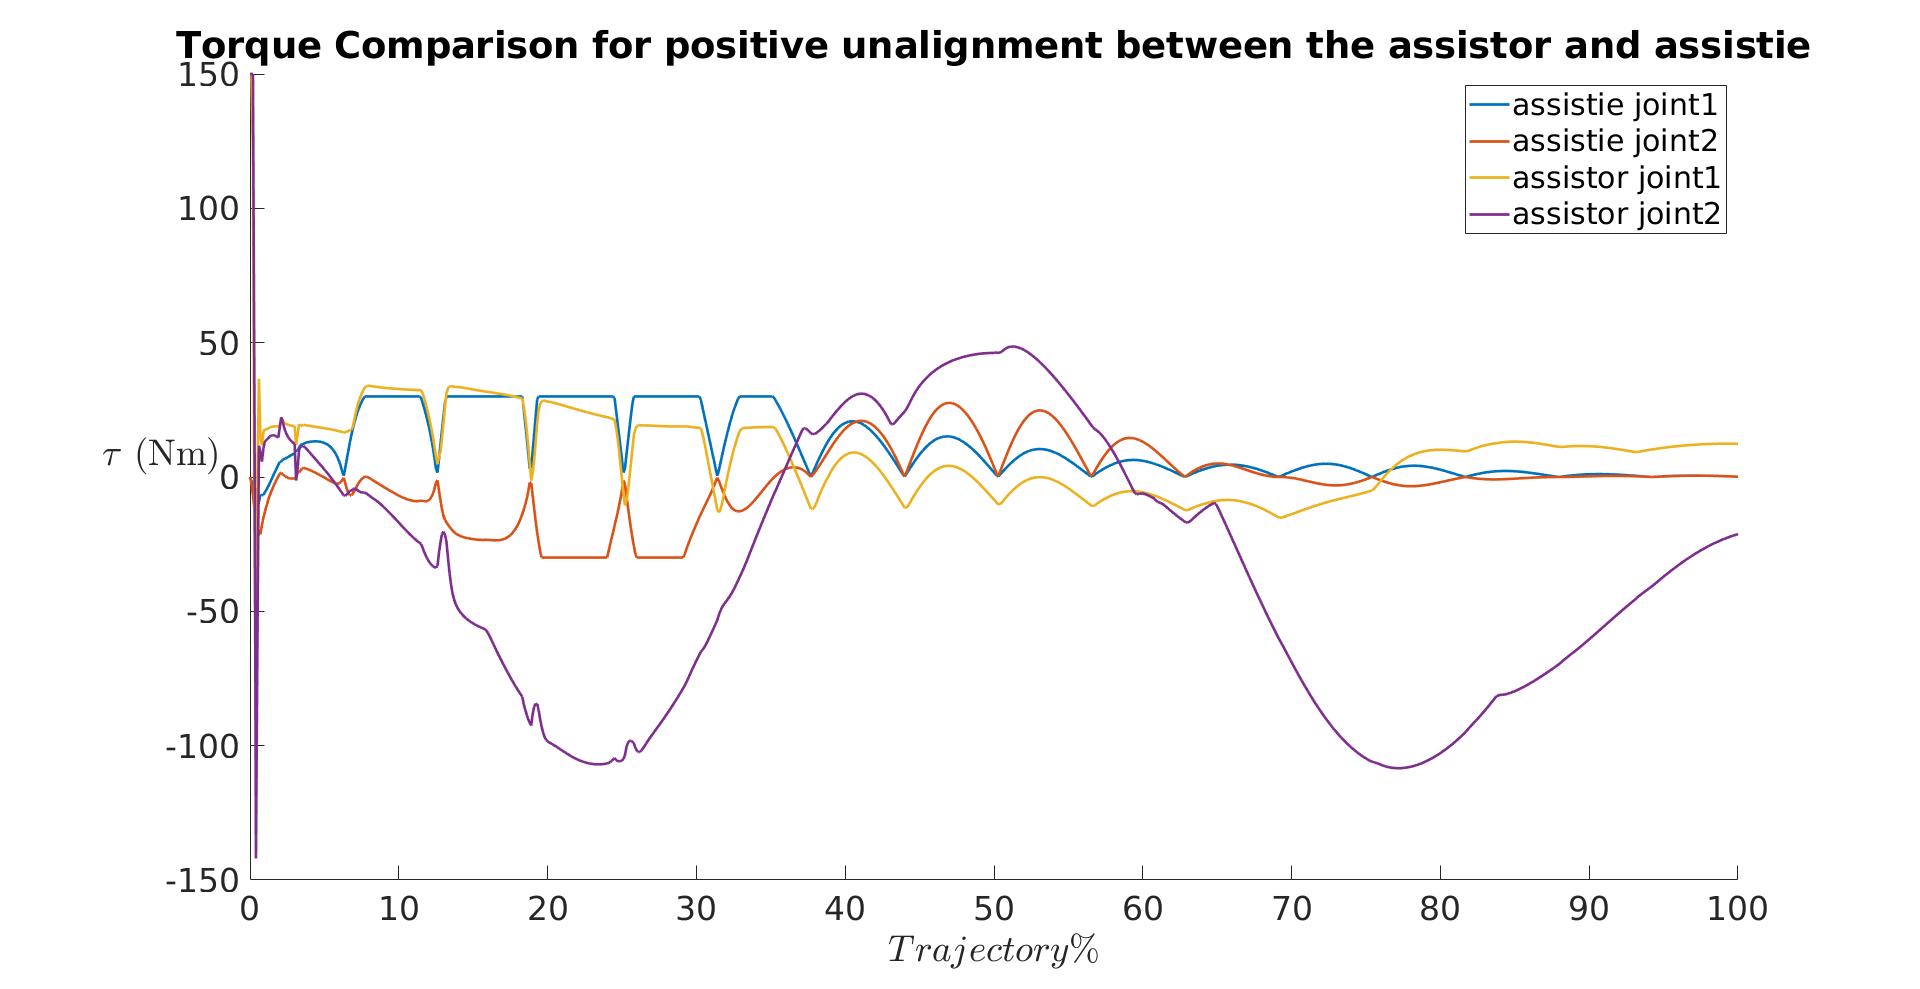
\includegraphics[width=\linewidth]{images/controllers/larger_length_torque.png}
        \caption[Double Pendulum: Positive Alignment-Effort]{Torque applied to the double pendulum}
        \label{fig:small_length_torque}
    \end{subfigure}%
    ~
    \begin{subfigure}{0.5\textwidth}
        \centering
        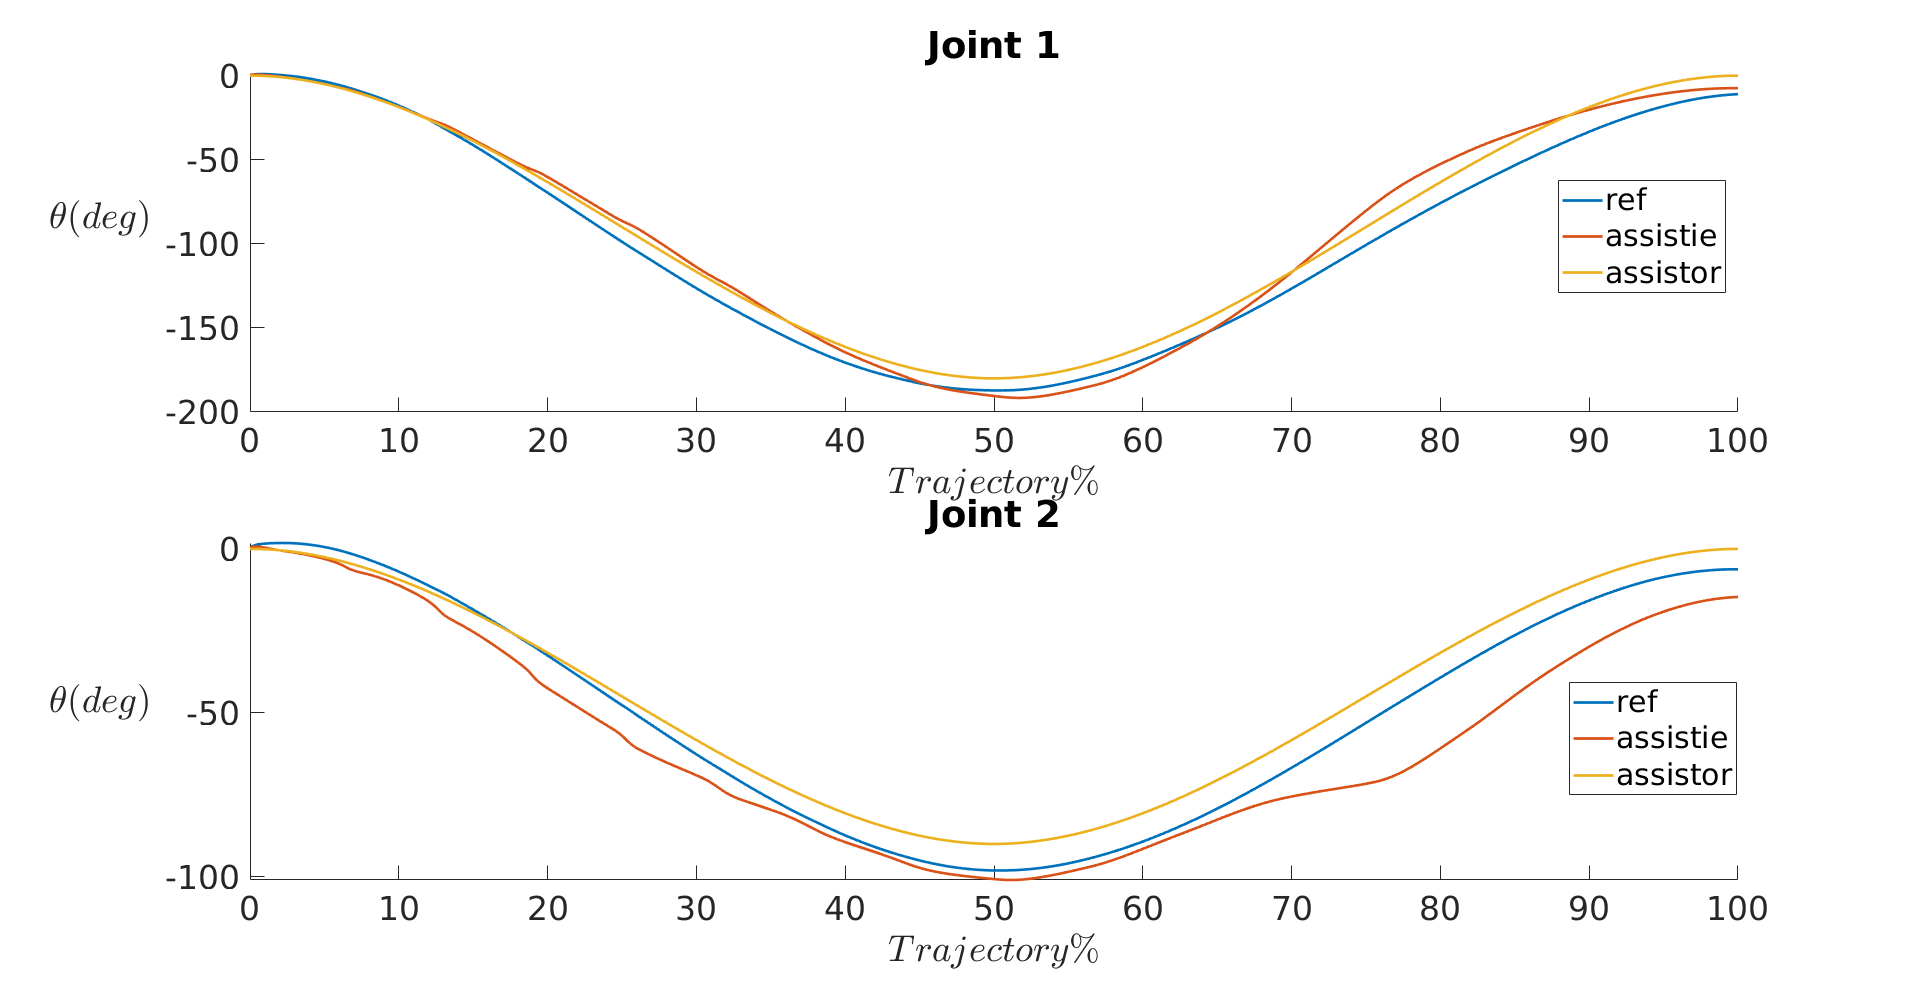
\includegraphics[width=\linewidth]{images/controllers/larger_length_traj.png}
        \caption[Double Pendulum: Positive Alignment-Trajectory]{Trajectories of double pendulum}
        \label{fig:small_length_traj}
    \end{subfigure}
    \caption[Double Pendulum: Positive Alignment]{Double pendulum model responses with at 1.05x of the human length \textit{assistie} torques.}
    \label{fig:larger_length}
\end{figure}


The controller performance increased by tuning the parameters of the SMC controller. The non-optimal parameters should have a significant deviation from the sliding surface. Using a cost function that considers velocity only has nearly the identical performance as the cost function that used both position and velocity; both performed better than the position only cost function. Using these results allows the velocity or the position and velocity to be good metrics for a cost function to tune the parameters of the A-SMC controller. The results show the importance of using the correct cost function to tune the controller gains. By selecting the wrong criteria for the tuning controller parameters, the controller will produce unstable results. It is important to note that the admittance controller parameters must be tuned in addition to the parameters of the SMC. If the variability parameters are too large, the admittance controller will lag/lead aggressively and not track the desired motion. 

\autoref{tab:error} summarizes the RMSE in degrees of the joint angles of the \textit{assistie} and \textit{assistor} systems. The largest error was caused with no  \textit{assistie} involvement. This is presumably caused by the non-rigid connection between the  \textit{assistie} and \textit{assistor} systems. The A-SMC controller does not have an understanding of the current state of the \textit{assistie} system, so it cannot directly control the position. However, since this was done in simulation, the error can be presented for comparison. The Sping-Dampener connection between the systems causes the \textit{assistie} to lag behind the \textit{assistie} system. Despite the \textit{assistie} it still only has an RSME error of $18.2^{\circ}$ on joint 1 and $16.7^{\circ}$ on joint 2; this is confirmed by examining the joint error of the reduced and time-varying simulations. The reduced test had the smallest RMSE, and the time-varying RMSE was between reduced and no-involvement simulations. 


Testing the variability in alignment allows for testing of the controller when the systems are not perfectly aligned. This problem arises for real systems where the person's joints may not align perfectly with the exoskeleton joints. As shown \autoref{fig:small_length} and \autoref{fig:larger_length} the tracking signals were close to the time-varying signals with only a slight variation in the tracking RMSE.


\begin{table}[h!]
\centering
 \begin{tabular}{||c |c c c c||} 
 \hline
    involvement  & \textit{assistor J1} & \textit{assistor J2} & \textit{assistie J1} & \textit{assistor J2}\\ [0.5ex] 
 \hline\hline
 None & 5.9^{\circ} & 9.5^{\circ} & 18.2^{\circ} & 16.7^{\circ} \\ 
 Reduced & 8.4^{\circ} & 6.3^{\circ} & 7.8^{\circ}  & 5.2^{\circ}\\
 Time Varying & 9.6^{\circ} & 6.2^{\circ} & 10.3^{\circ}  & 9.6^{\circ}\\ 
 0.95x length & 9.9^{\circ} & 6.6^{\circ} & 10.0^{\circ}  & 9.4^{\circ}\\
 1.05x length & 9.3^{\circ} & 6.3^{\circ}  & 10.7^{\circ}   & 9.8^{\circ}  \\[1ex] 
 \hline
 \end{tabular}
 \caption{Joint RSME in degrees}
  \label{tab:error}
\end{table}





\subsection{Application of Tuning Methodology on a Simple Trajectory}

The tuning methodology discussed above was implemented on a the leg of the LARRE using the dynamics server to calculate the inverse and forward dynamics. This was due to complicated in the ROS-Simulink bridge, which is discussed below. 

To tune the controller each of the joints of the leg where command to follow a polynomial trajectory. This was done to allow for the boundary conditions of the path to be controlled for testing. The tuning method discussed above. This model added complexity to tuning process since it added another dimension that need to be tuned. An assumption that was made that while the thigh and shank of the exoskeleton where connected via a spring-dampener system, the foot of the exoskeleton and human where rigidly connected. Additionally, the closed loop PD controller is assumed to be a FES type devices that can transform displacement into torque through pulse width and frequency modulation \cite{rouhani2017pid, ha2015approach,Model_Ferrarin}. The hip and knee joints of the exoskeleton controller is assumed to be powered by BLDC motors as discussed in \autoref{chap:mech}.

\autoref{fig:LARRE_TUNING} shows the cost convergence over the optimization. A single leg was tuned to lower the amount of parameters that needed to be optimized. The optimization lowers the RSME cost from 2.66 to 0.6 which is a 77.44\% reduction. At each step in the iterations the parameters are changed in attempt to lower the cost function. The parameters being tuned have different magnitudes are thus graphed in separately to accurately show the change at each step. \autoref{fig:LARRE_Train_Trajectory} shows how the joints of the training trajectories. As shown the initial starting position has some wobbling in the ankle position be the converged to the desired trajectory. This can be due to the initial conditions in the admittance controller or the value of $\lambda$ being large which effect the rise time.  

\begin{figure}
    \centering
    \begin{subfigure}[b]{\textwidth}
        \centering
        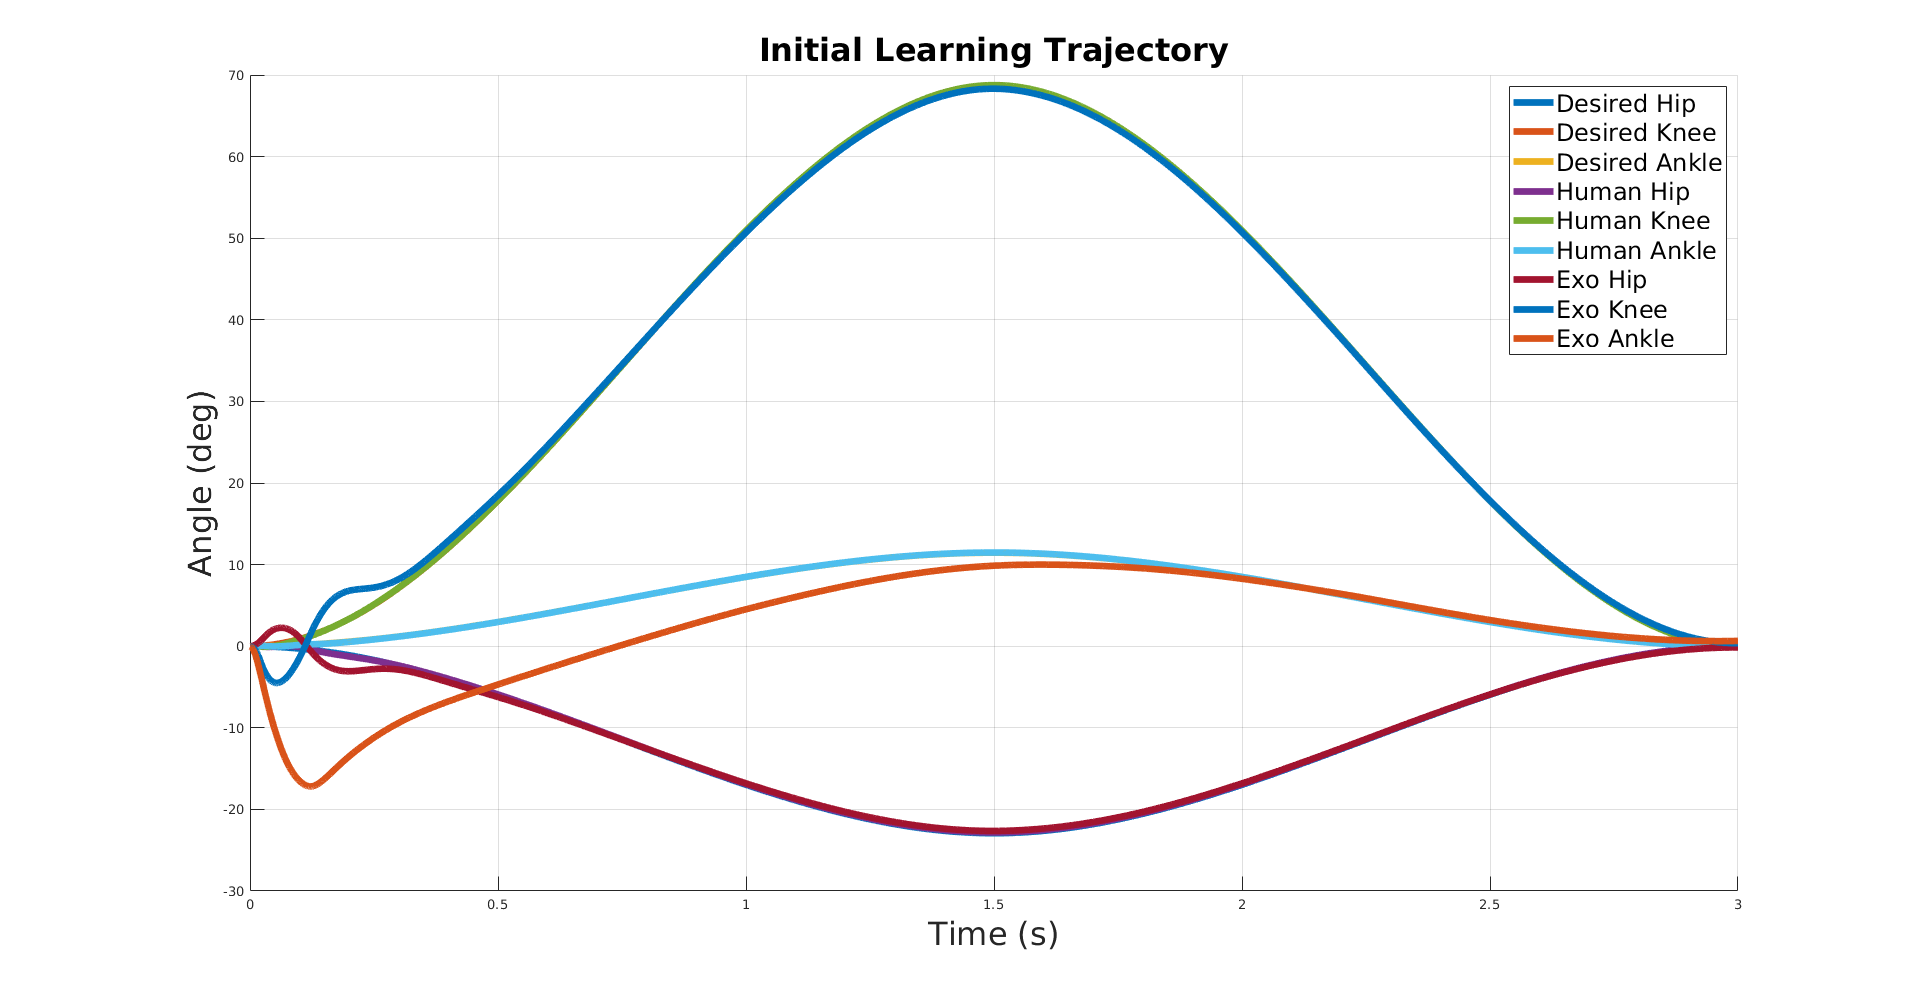
\includegraphics[width=0.8\columnwidth]{images/controllers/trajs/init_traj.png}
        \caption[LARRE Training Trajectory]{LARRE Training Trajectory}
        \label{fig:LARRE_Train_Trajectory}
    \end{subfigure}
    
    \begin{subfigure}[b]{\textwidth}
        \centering
        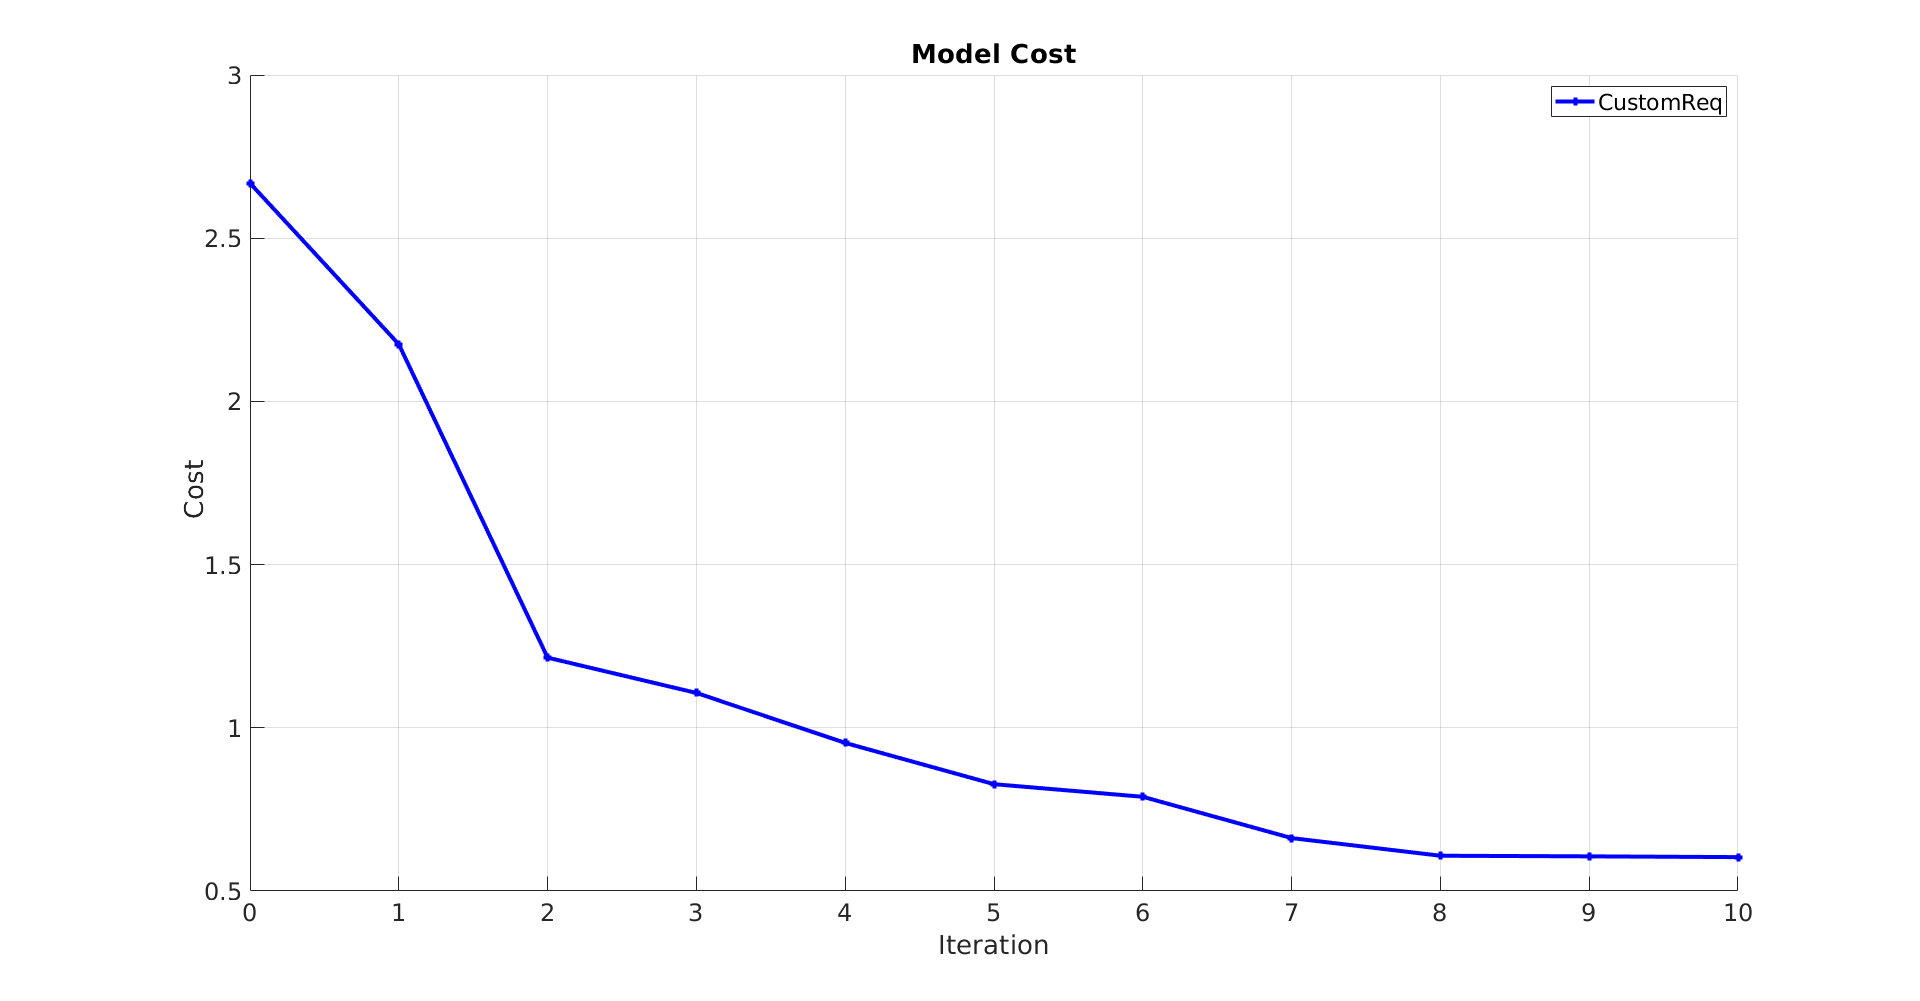
\includegraphics[width=0.8\columnwidth]{images/controllers/trajs/cost.png}
        \caption[LARRE Cost Optimization]{Cost of Tuning a single leg of LARRE}
        \label{fig:LARRE_TUNING}
    \end{subfigure}
  
    \begin{subfigure}[b]{\textwidth}
        \centering
        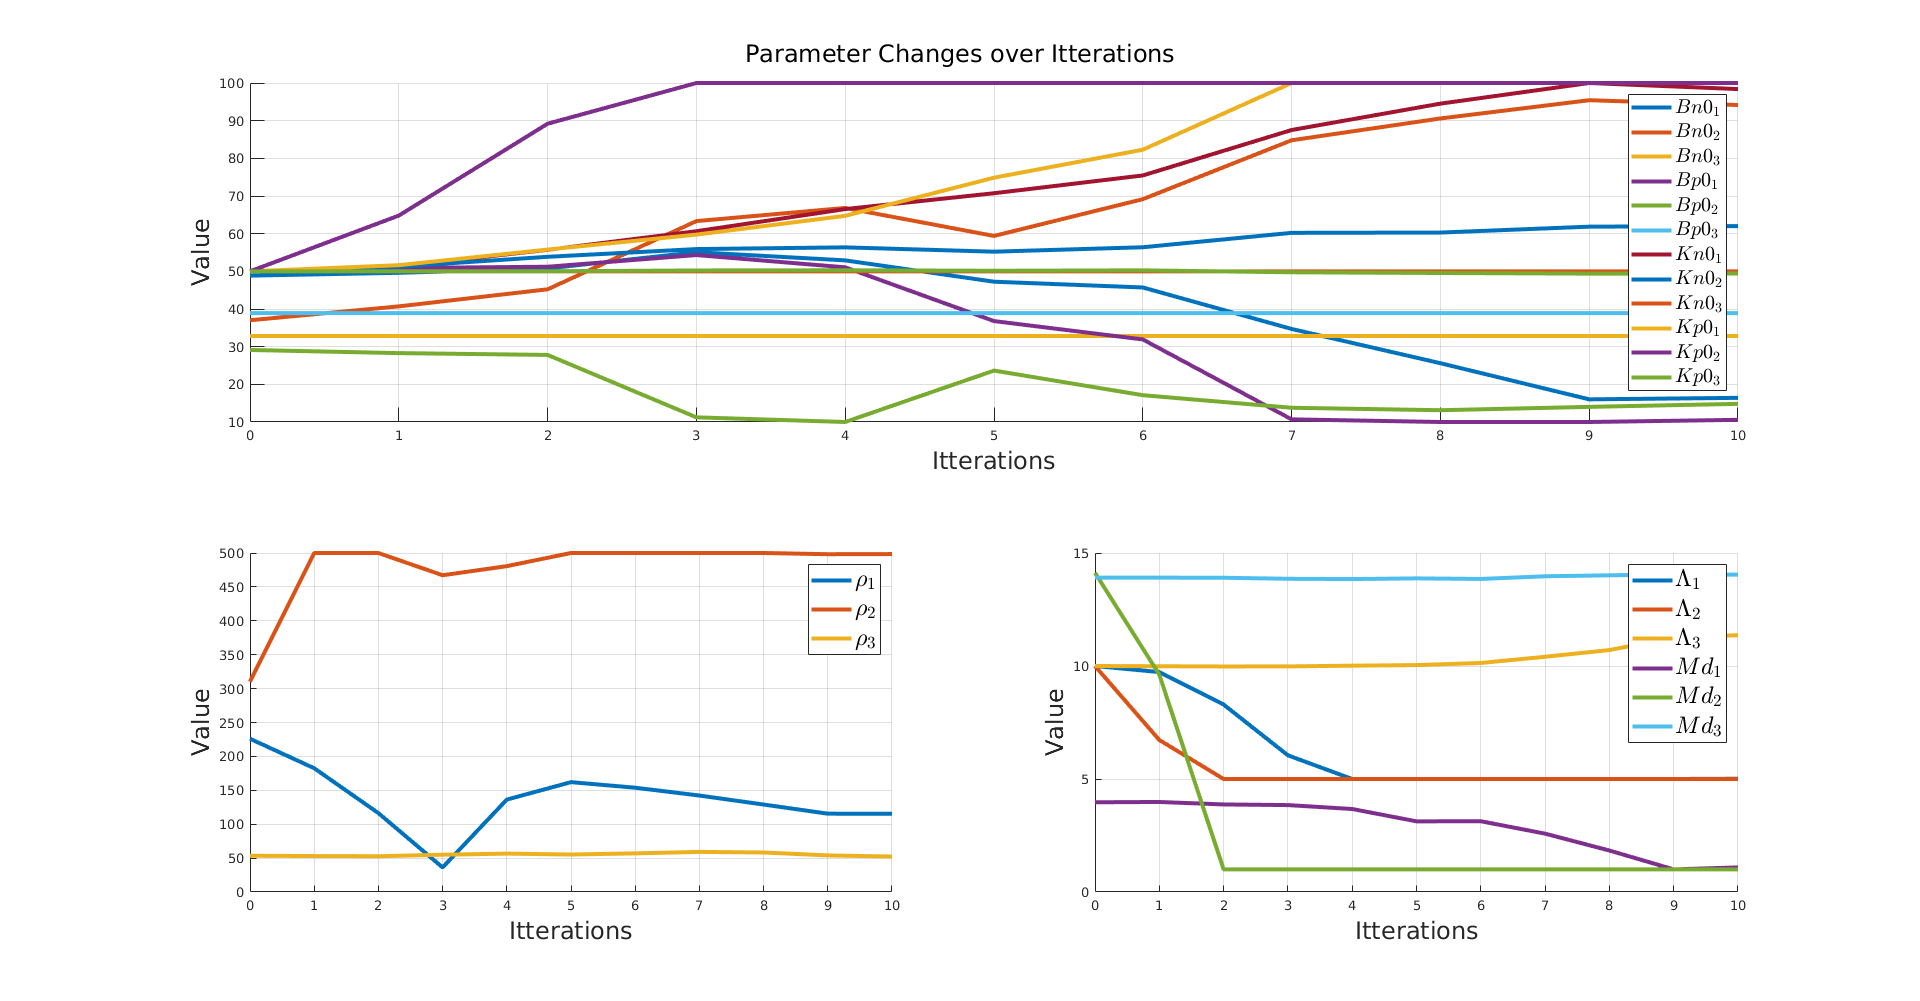
\includegraphics[width=0.8\columnwidth]{images/controllers/trajs/params_splite.png}
        \caption[LARRE Parameters Optimization]{Parameters Changing Over Iterations}
        \label{fig:LARRE_PARAMS}
    \end{subfigure}

    \caption{Output for Training LARRE Graphs}
    \label{fig:traj_training_graph}
\end{figure}


While \autoref{fig:LARRE_PARAMS} shows how the parameters change over time it does not give insight to the relative importance of the tuning parameters. A global sensitivity analysis was done to examine which parameters have the largest effect on the cost function. The goal of the analysis is to apportioning the uncertainty in outputs to the uncertainty. A global sensitivity analysis is when all the parameters are varied simultaneously over the entire range of the the inputs factors \cite{saltelli2008global}. This can be done by examining several different correlation methods listed below. Additional, these methods can also be examined as \textit{Ranked} methods. A ranked correlation method measures an ordinal association between the different variables. The ranking is is the assignment of the ordered labels. 

\begin{itemize}
    \item \textbf{Correlation}: Statistical relationship between two variables. 
    \item \textbf{Kendall}: Measure the ordinal association between two measured quantities \cite{abdi2007kendall}.
    \item \textbf{Standardized Regression}: A regression analysis where the underlying data is standardized so the variance of dependence can be compared \cite{SIEGEL2016355}.  
    \item \textbf{Partial Correlation}: Measures the degree of association between two random variables, with the effect of a set of controlling random variables removed \cite{PARTIALCORRELATION}. 
\end{itemize}




\autoref{fig:paramStats} shows the relative importance of the parameters, here the graphs is defined between -1 and 1. The closer the value is to $\|1\|$ the higher its sensitivity Where a 1 indicates that changing that parameters will increase the cost function and a value closer -1 indicates that changing the parameter will lower the cost function.

This data can be used to choose the more important parameters when optimizing the system. This is important for systems with a large number of parameters. Examining the results indicates the variable $M_d$ have a little impact on the cost function. This low impact is expected since the $M_d$ variable is a constant post multiplier the $K_d$ and $B_d$ terms (see \autoref{eq:addmittance}-\autoref{eq:varible}). The relative high importance of $\rho$ can be explained by its effect on the SMC. The $\rho$ are with the sliding mode gains, which controls the chattering in the system as show in \autoref{eq:SMCChattering}, where $T_s$ is the time and $\Delta$ is the chattering. The $\alpha$ parameter controls how the variable admittance controller reacts. Changes to this varible will impact the value of the $Kn$ and $Kp$ gains, which also have a relative high importance which controls the torque to generate for a difference in position between the two systems. If the two systems drift apart the controller increase the gain to align the systems. In contrast the $Bn$, $Bp$, and $\gamma$ terms have relatively low importance which indicates that the two systems generally had the same velocity so increase the gains had little effect on the system. 



\begin{equation}
    \Delta = \rho T_s
    \caption[SMC Chattering]{SMC Chattering}
    \label{eq:SMCChattering}
\end{equation}


\begin{figure}
    \centering
    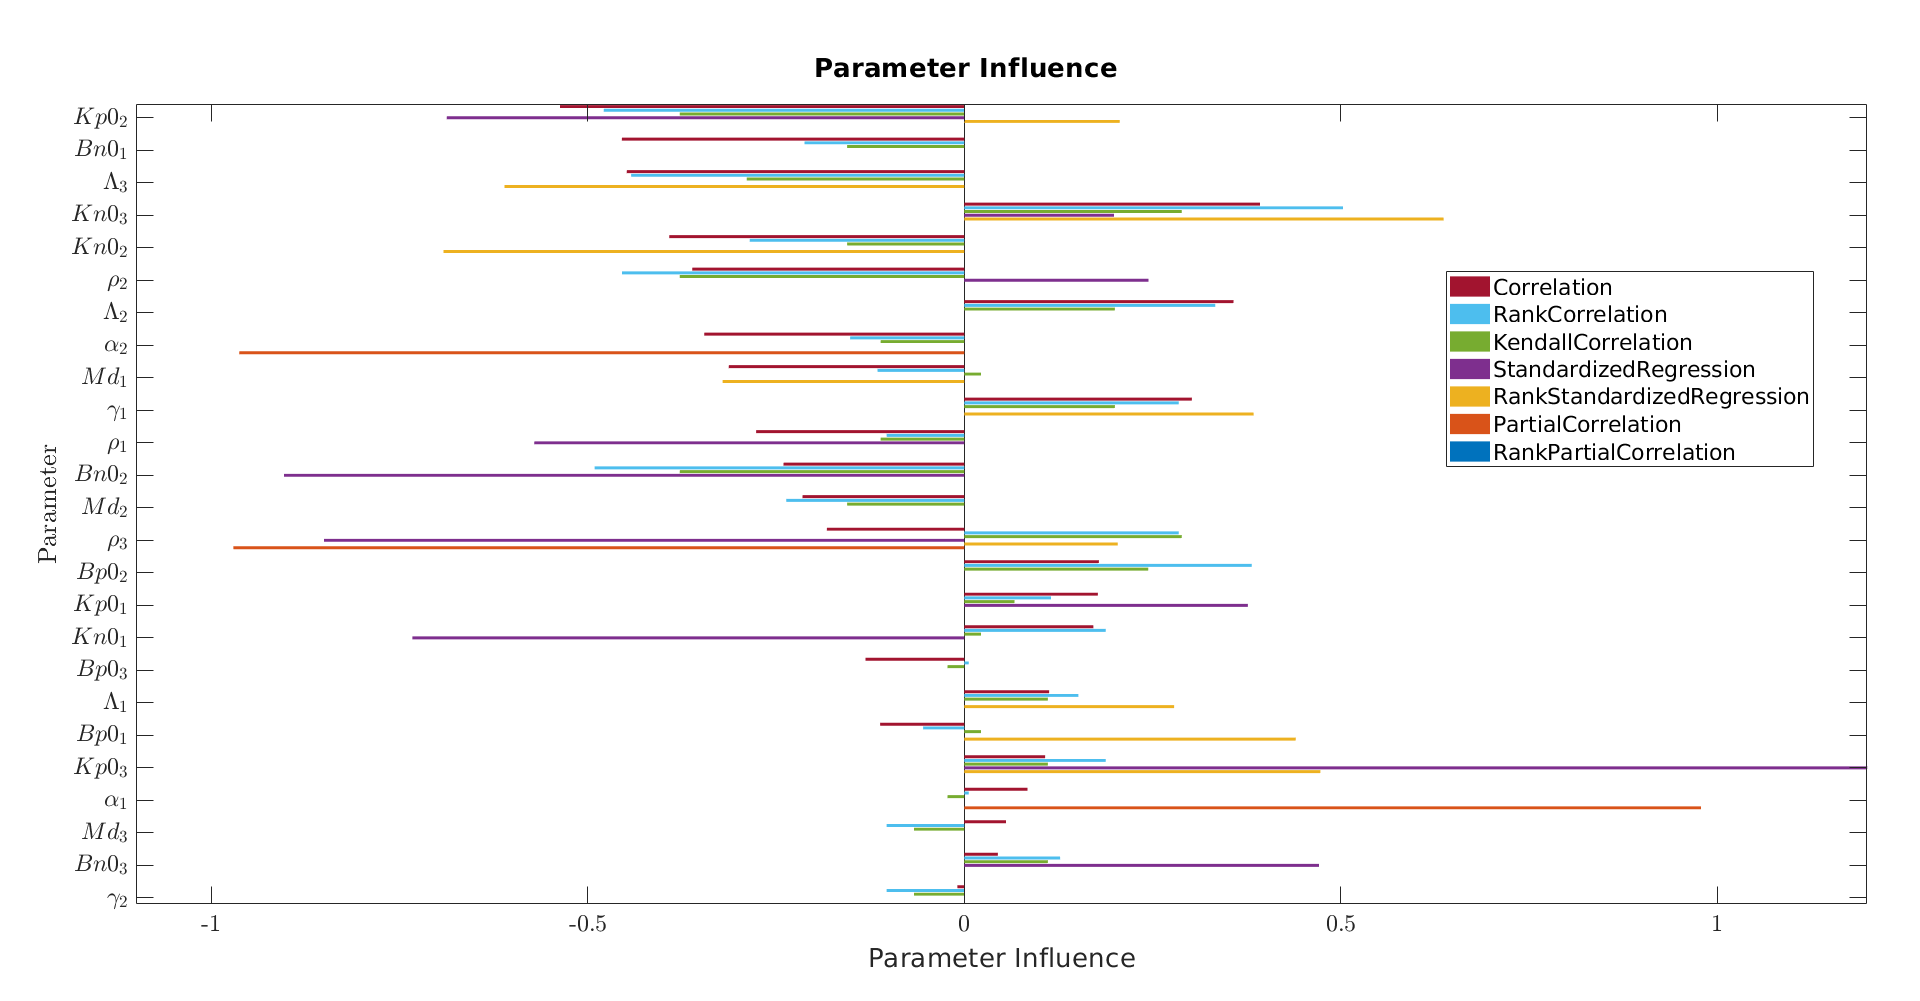
\includegraphics[width=\columnwidth]{images/controllers/trajs/stats.png}
    \caption[Relative Parameters Importance]{Relative Parameters Importance}
    \label{fig:paramStats}
\end{figure}



To examine the effect of the the model gains and the ability of the controller to adapt to to varying human interaction. The same trajectory was repeated three times. This was done to show how the steady state behavior of controller. Additionally, the foot is omitted since it is considered to be rigidly attached to the exoskeleton foot. 
To examine the effects of the human effort were applied to the system from full human interaction to zero human interaction including 80\% involvement, 50\% involvement, 20\%, and a time decaying involvement. The percentage involvement was defined by examine the torque generated at 100\% involvement which was approximate $10Nm$. 

\autoref{fig:StateSpaceTrajectory} shows the state space of the hip and knee joint. They show the joints move towards the sliding surface and converge towards zero with minimal chattering.  As shown in \autoref{fig:TripleTrajectory} the initial start part of the trajectory takes some time to settle to the trajectory. After the initail part of the motion the settles. The hip motion is slightly off the desired motion. The exoskeleton torque was capped to not exceed a maximum which should be raised to track the motion. This is shown since the knee motion tracks smoothly. 




\begin{figure}
    \centering
    \begin{subfigure}{\linewidth}
        \centering
        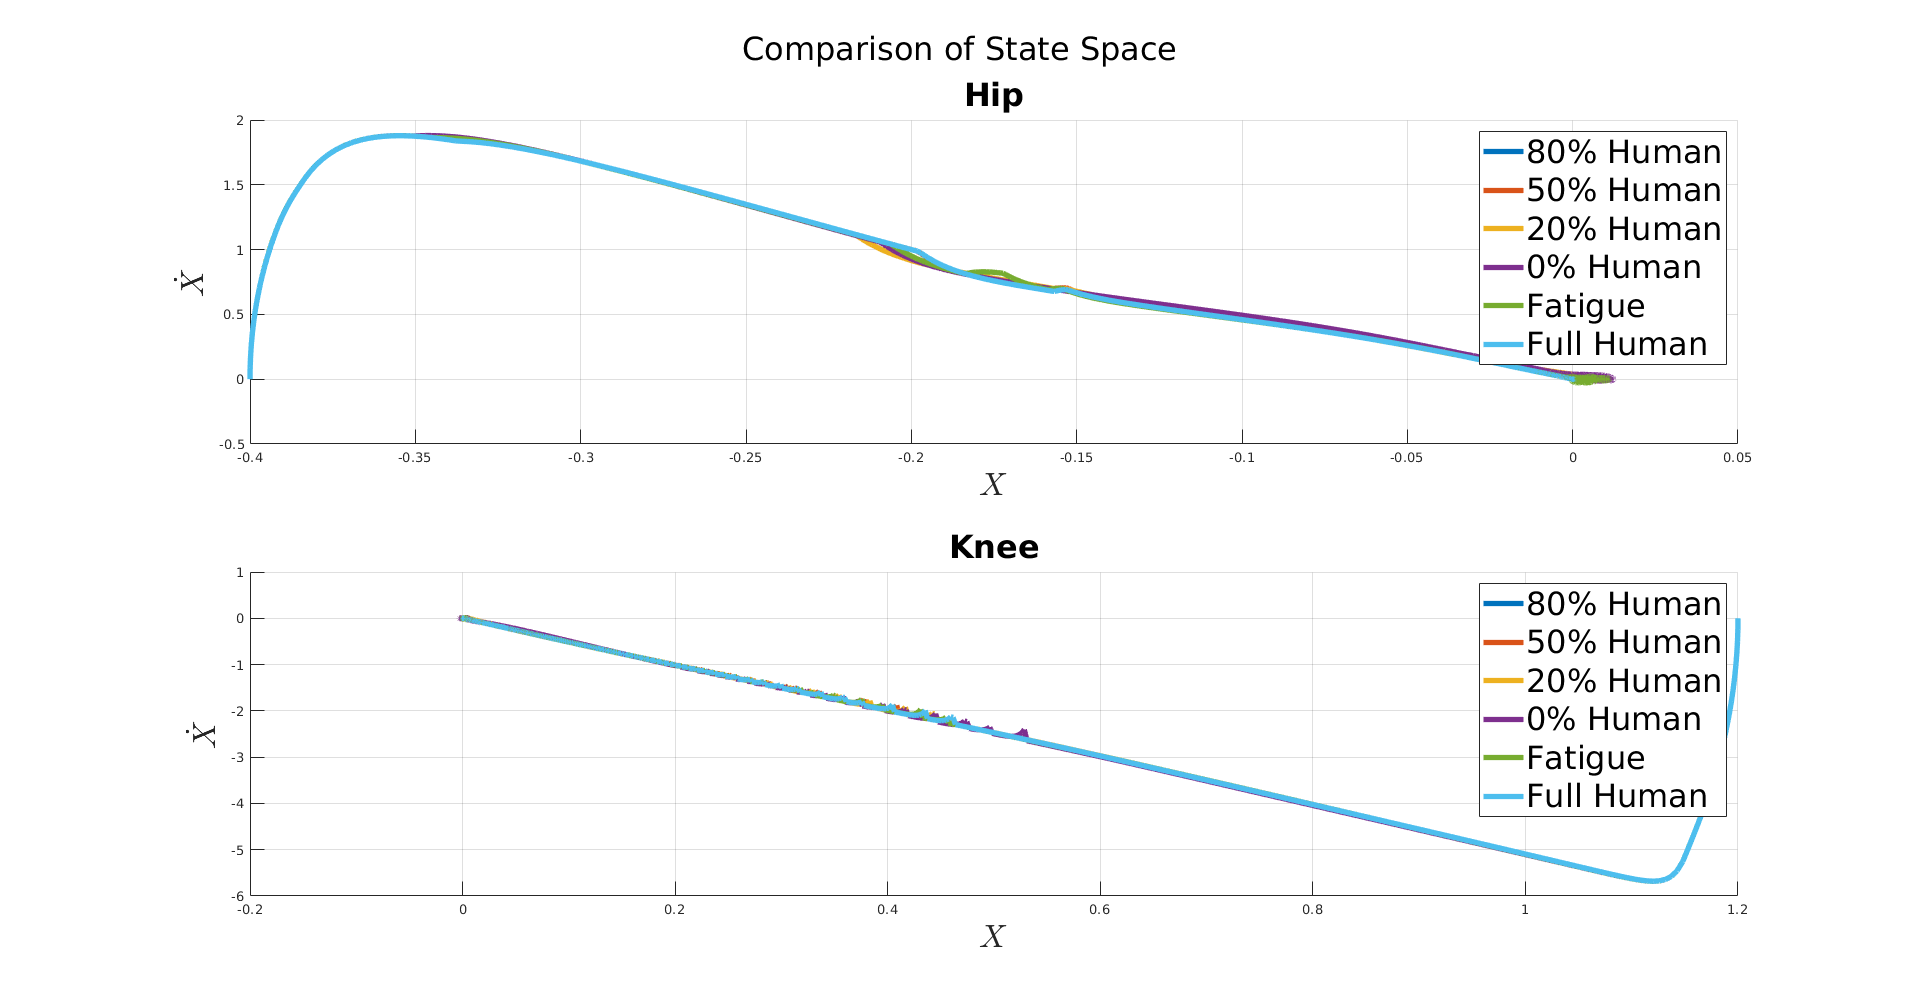
\includegraphics[width=\columnwidth]{images/controllers/trajs/statespace.png}
        \caption[State Space Trajectory]{State Space Trajectory}
        \label{fig:StateSpaceTrajectory}
    \end{subfigure}
    \begin{subfigure}{\linewidth}
        \centering
        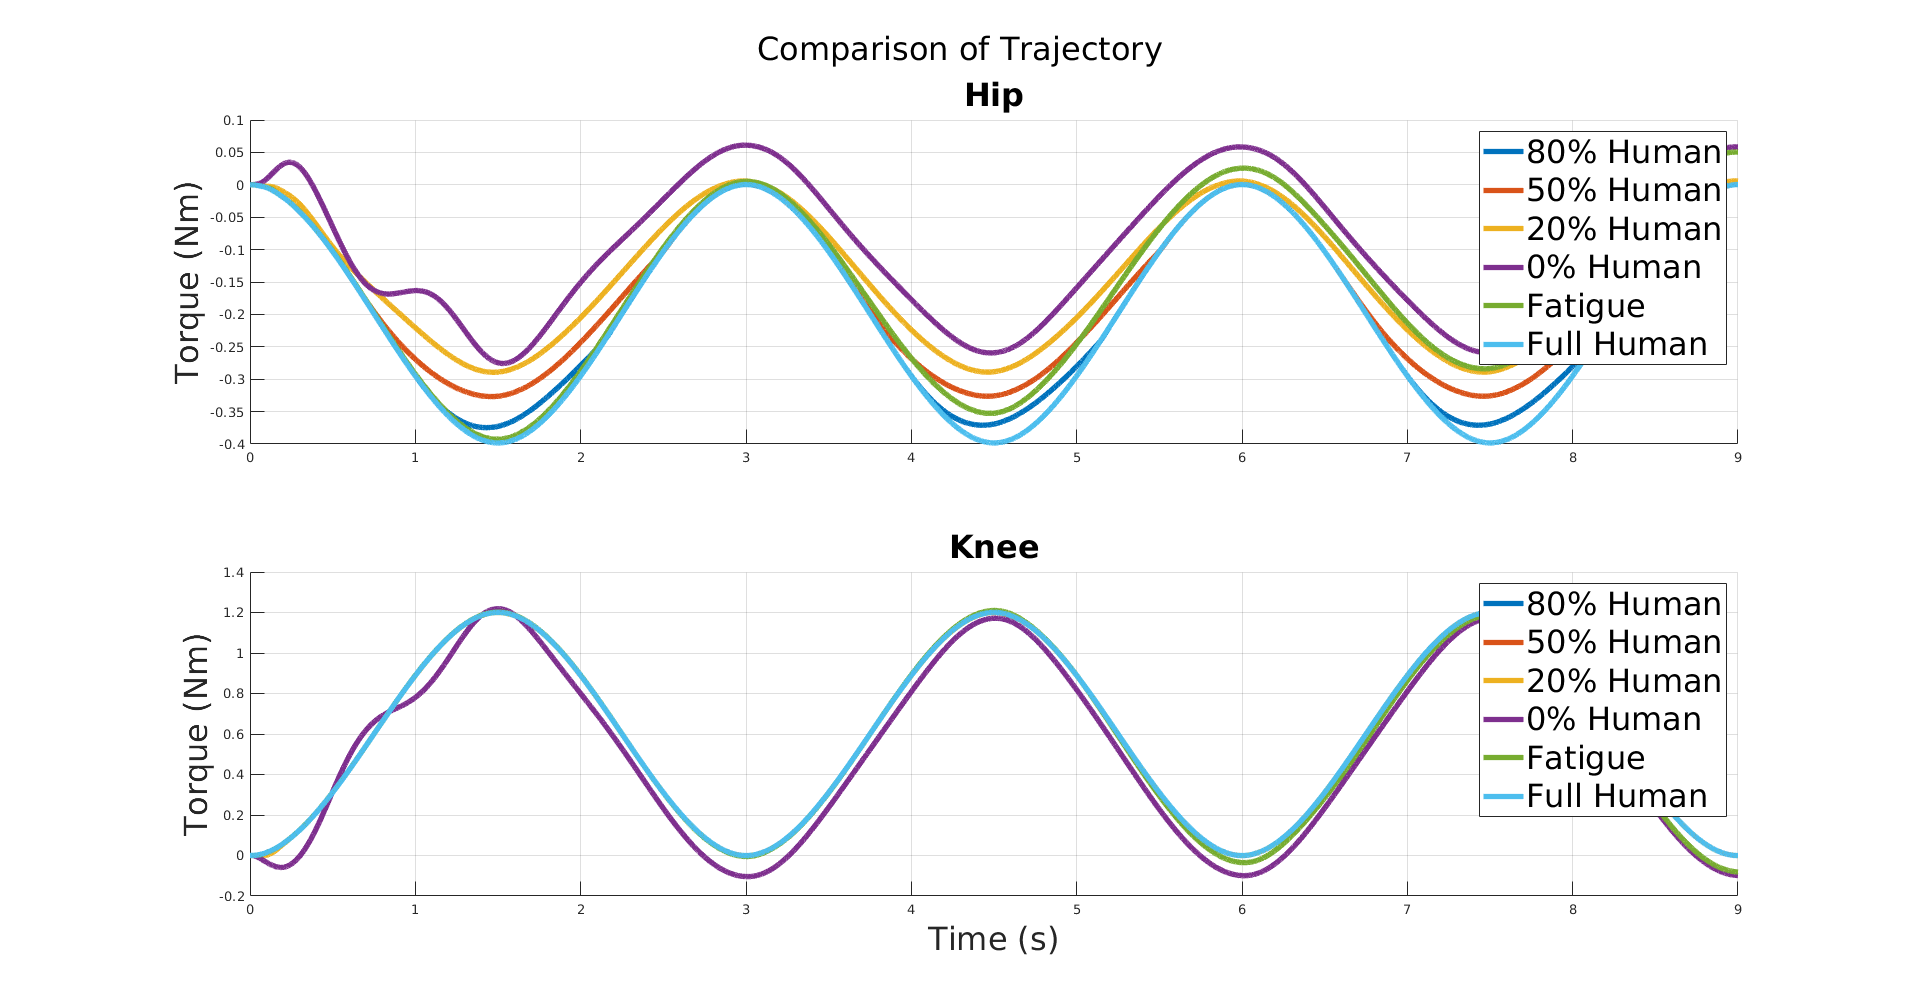
\includegraphics[width=\columnwidth]{images/controllers/trajs/triple_traj.png}
        \caption[Triple Trajectory]{Triple Trajectory}
        \label{fig:TripleTrajectory}
    \end{subfigure}
    \caption[Triple Trajectory LARRE]{Triple Trajectories}
    \label{fig:TripleTraj}
\end{figure}



The human interaction is shown in \autoref{fig:humantripletraj}. For the varying interaction levels the human effort was saturated, this is shown since the toque cannot exceed the capped value. The fatigue started at 80\% human interaction and reduced as an exponential sine wave to 0\% interaction as shown in \author{fig:fatprofile}. While this may not be an accurate model it represents a decreasing torque over time. Additional fatigue is difficult to model as it depends on the patient muscle atrophy, the muscle being activated, and the pulse width used to activate the muscle \cite{reiner1998patient}. As expected the fatigue interaction contains a wave like motion as the PD controller attempts to handle the varying engagement levels. 


\begin{figure}
    \centering
    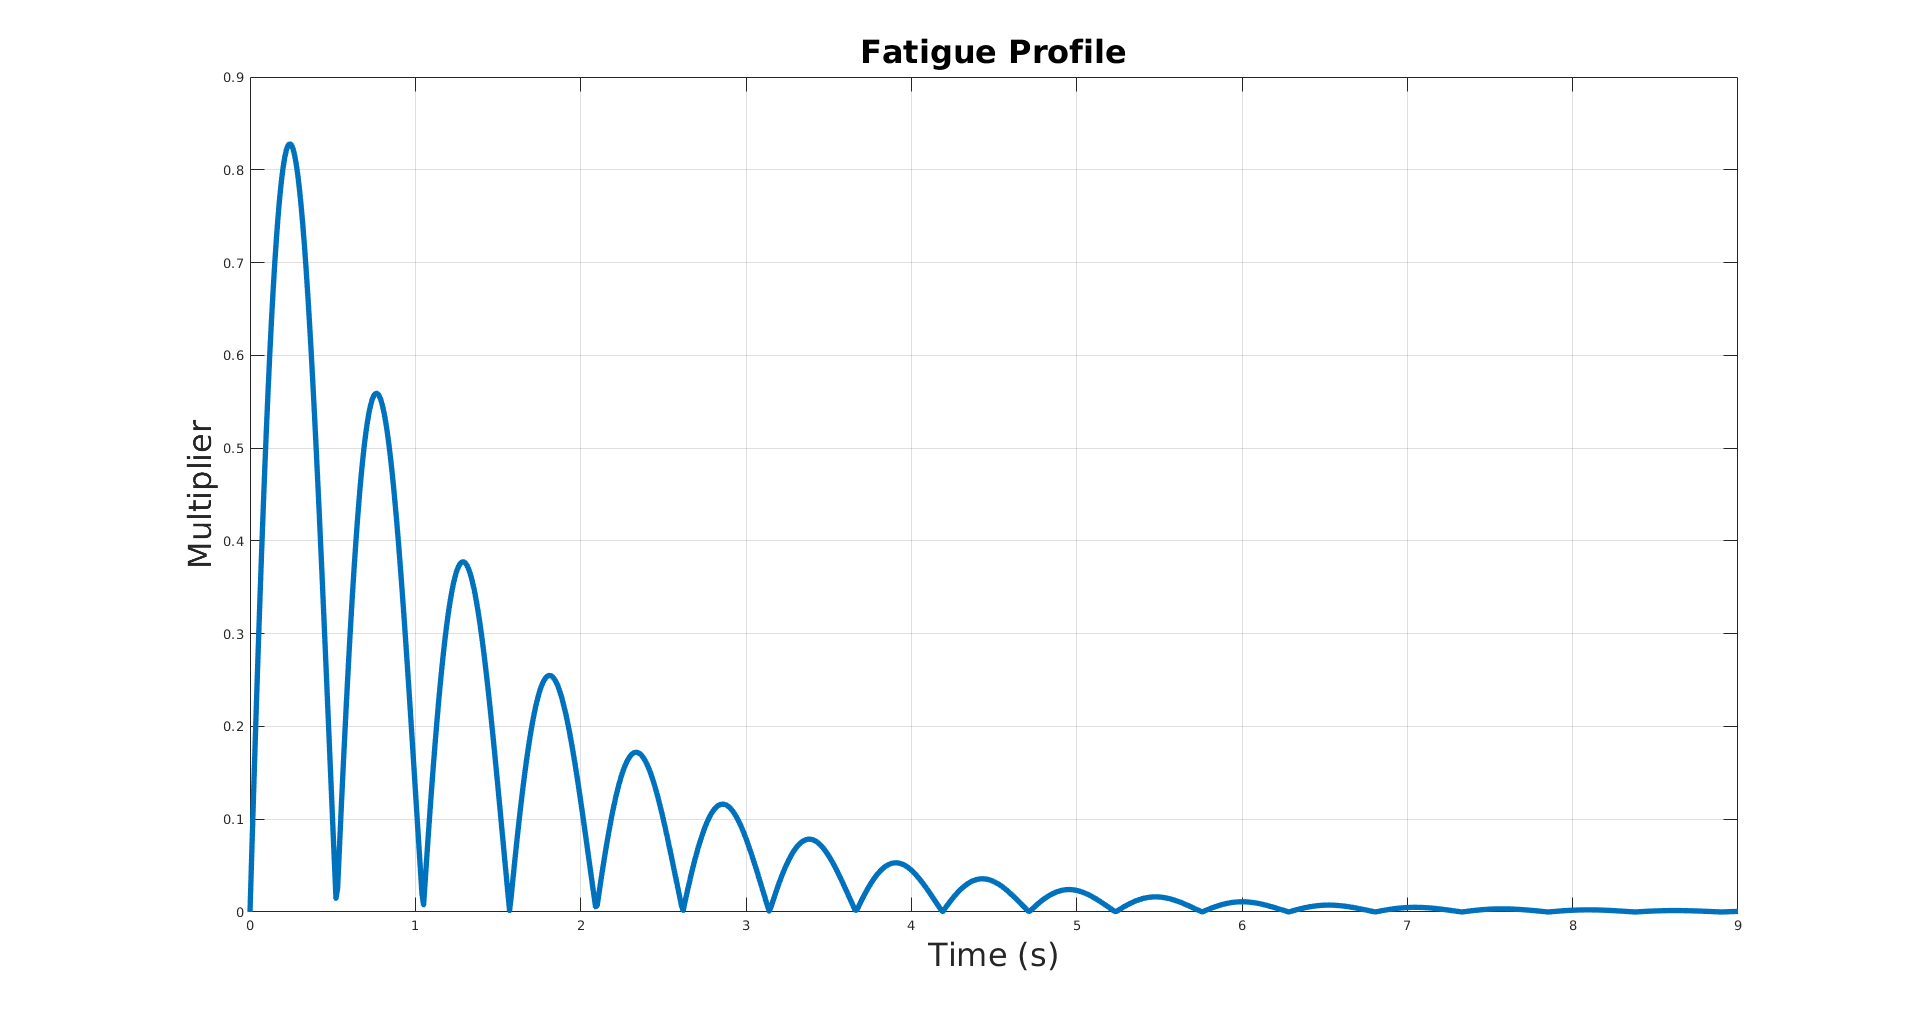
\includegraphics[width=\columnwidth]{images/controllers/gait/fat_profile.png}
    \caption[Fatigue Profile]{Fatigue Profile}
    \label{fig:fatprofile}
\end{figure}


\begin{figure}
    \centering
    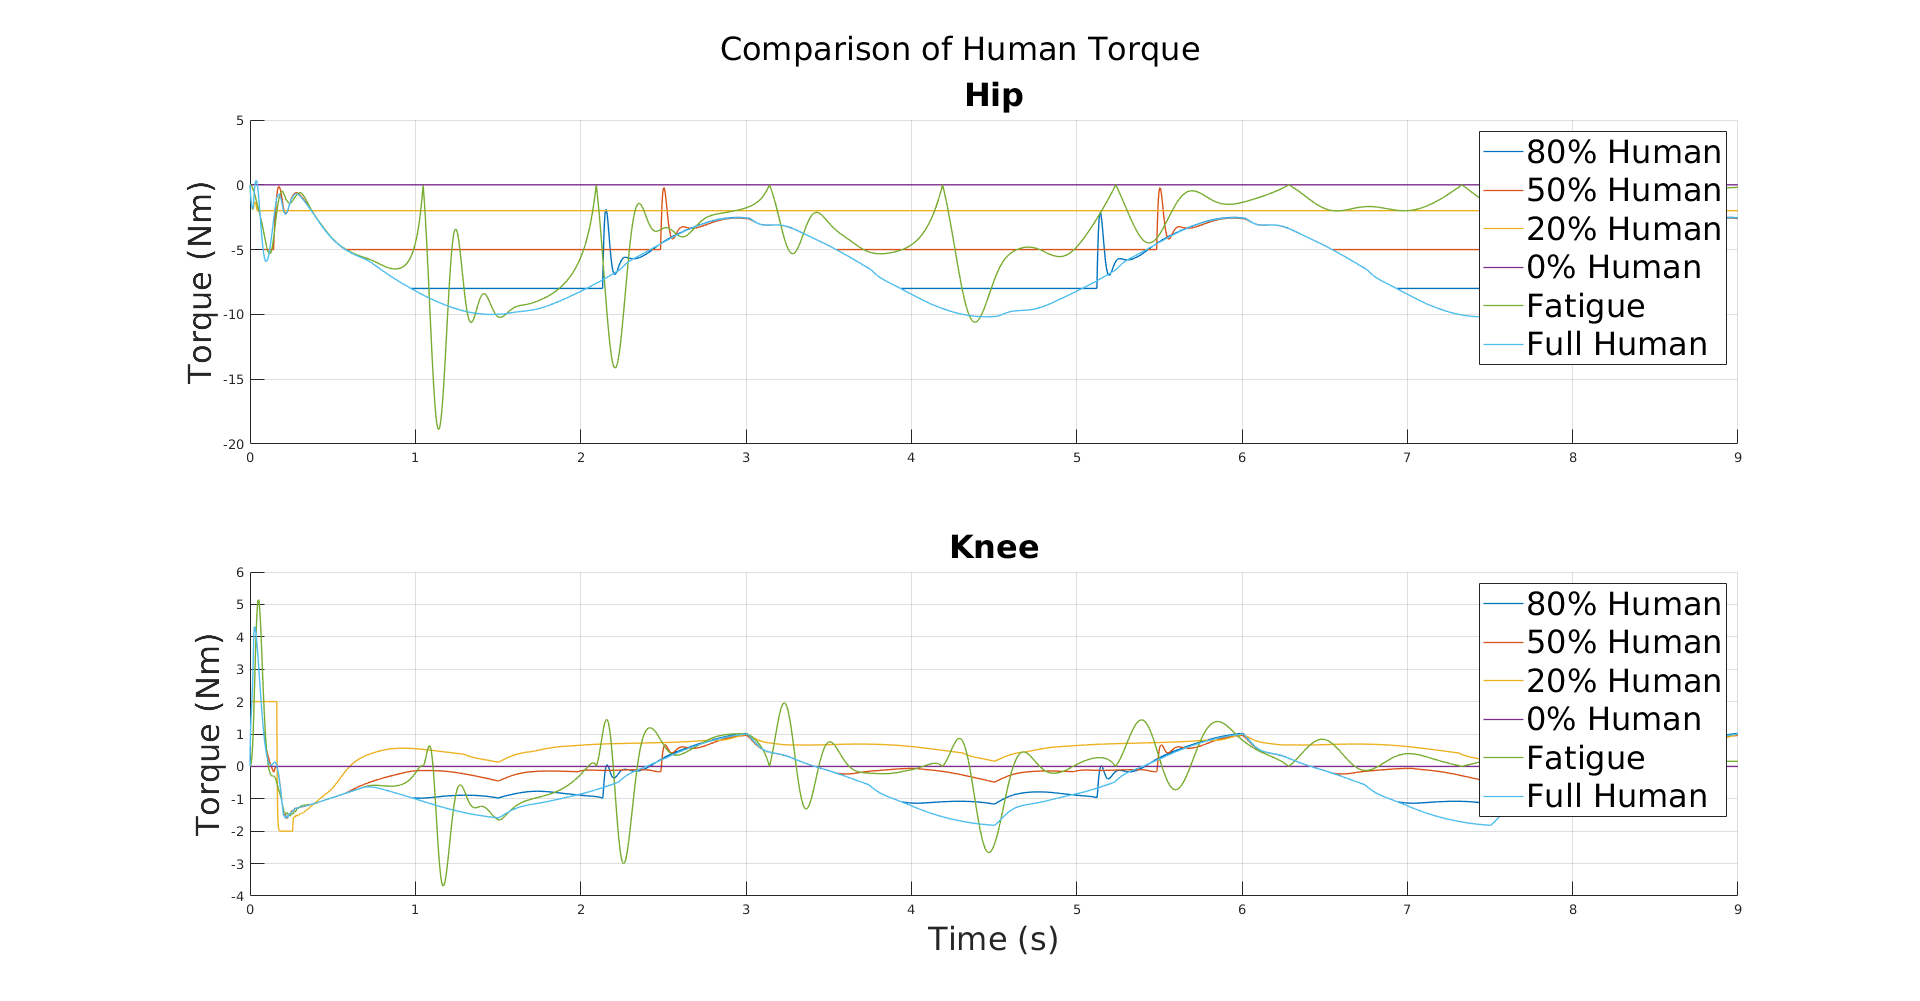
\includegraphics[width=\columnwidth]{images/controllers/trajs/human.png}
    \caption[Human Torque over Triple Trajectory]{Human Torque over Triple Trajectory}
    \label{fig:humantripletraj}
\end{figure}


\autoref{fig:SMCTripleFull} shows the effort supplied by the SMC for each of the engagement levels. \autoref{fig:SMCTripleZoom} is a zoomed of the same graph. As shown the as the human engagement increased the SMC magnitude of the effort decreased for both hip and knee joints. This shows that the SMC controller is adapting the human engagement level. 


\begin{figure}
    \begin{subfigure}{\linewidth}
        \centering
        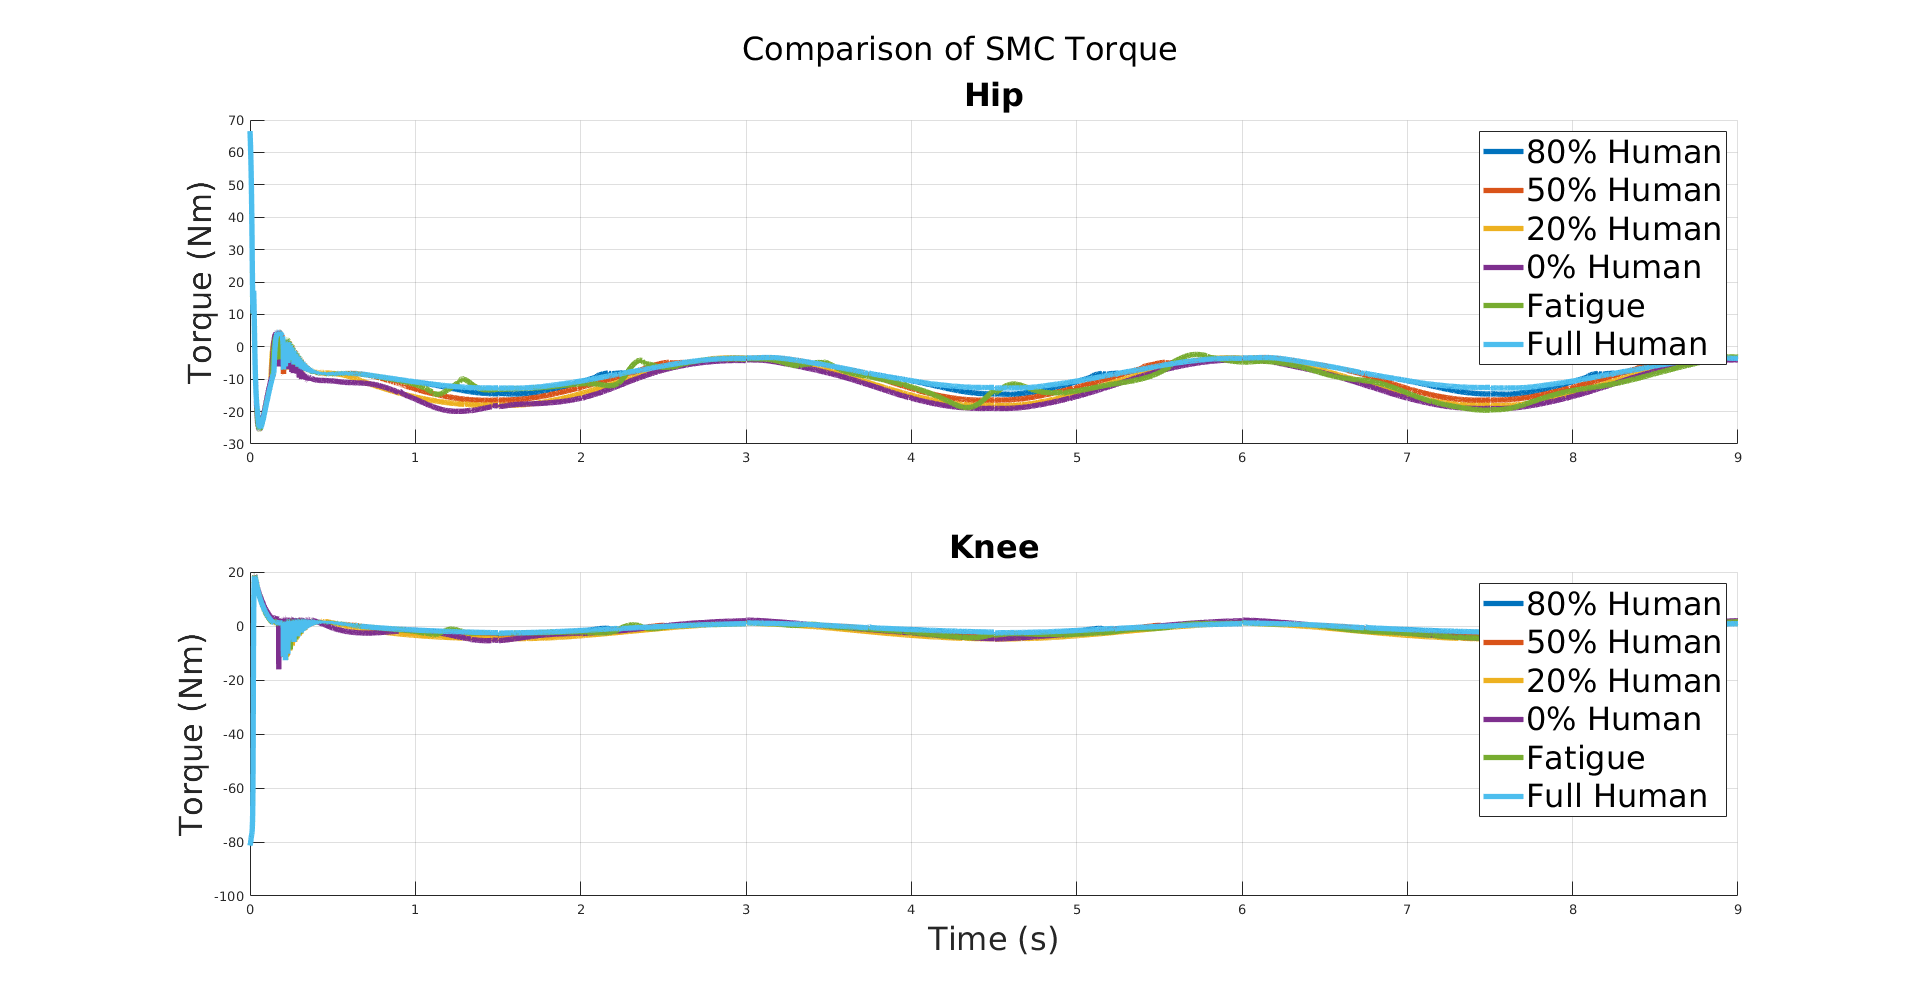
\includegraphics[width=\columnwidth]{images/controllers/trajs/SMC_full.png}
        \caption[SMC Torque over Triple Trajectory]{SMC Torque over Triple Trajectory}
        \label{fig:SMCTripleFull}
    \end{subfigure}
    \begin{subfigure}{\linewidth}
        \centering
        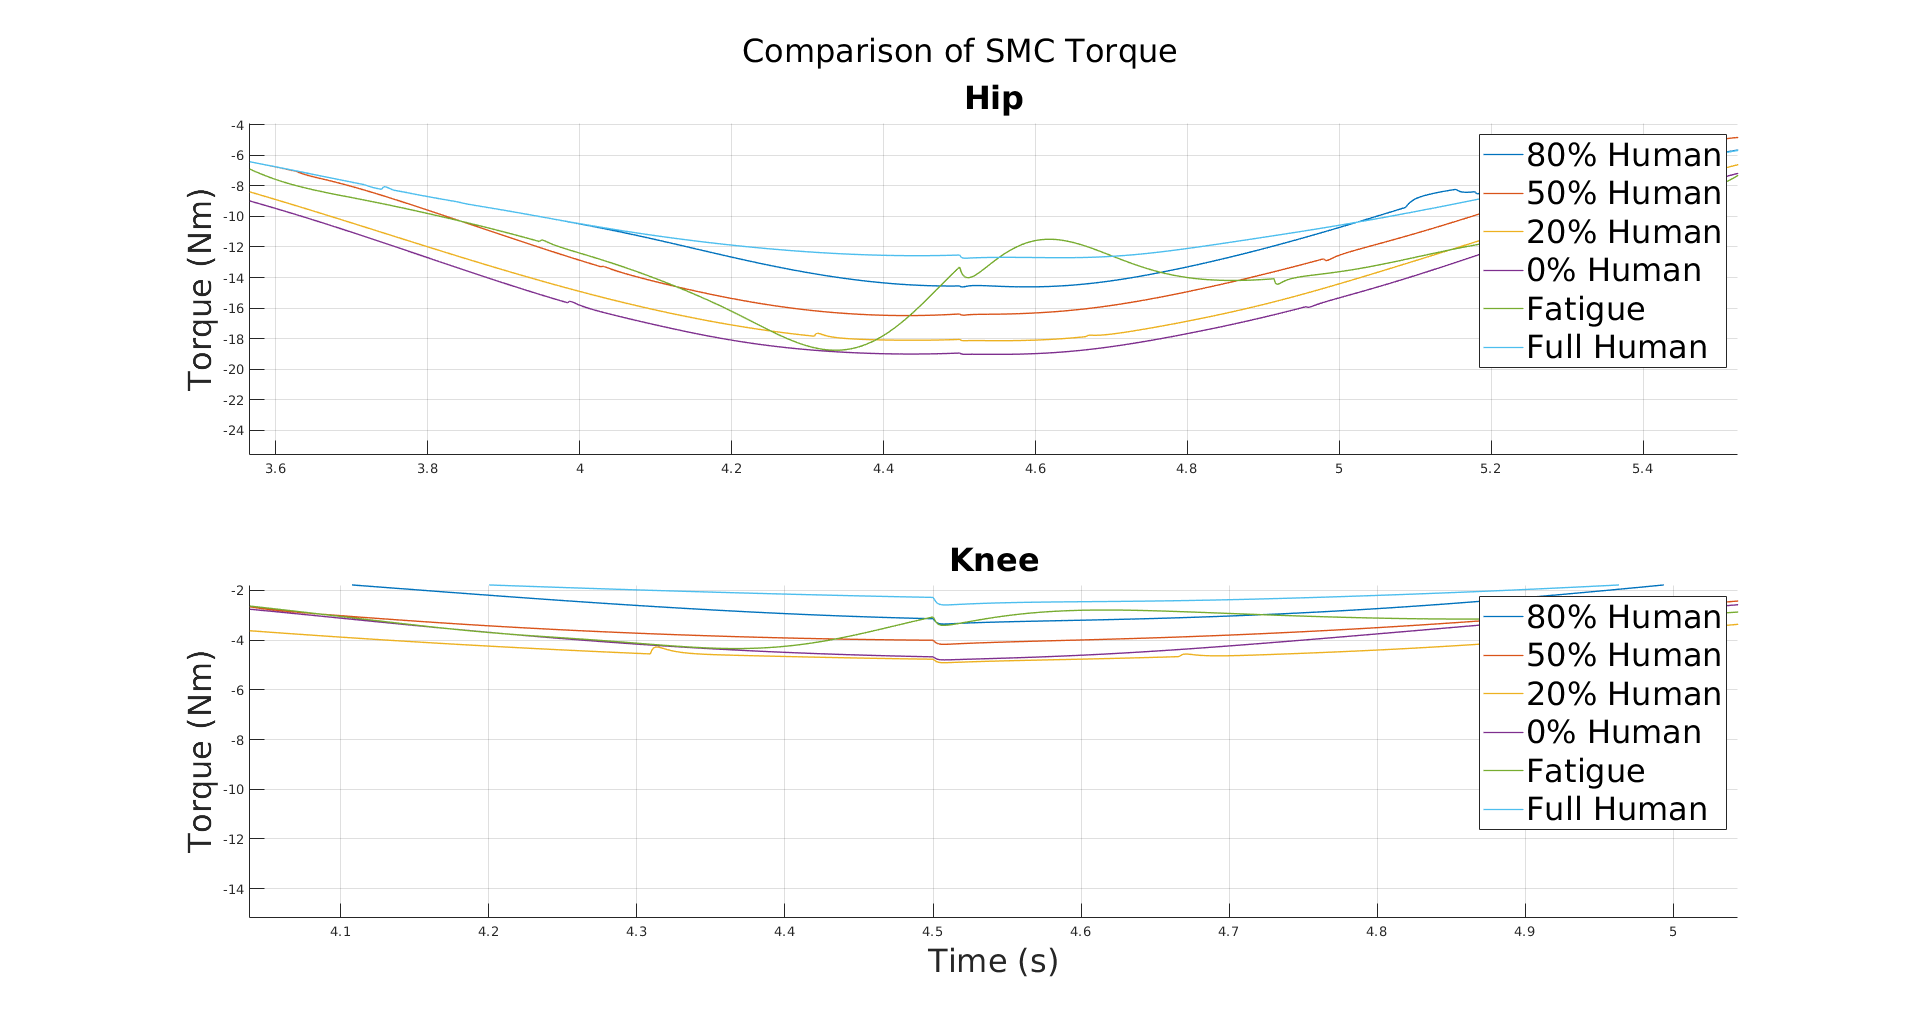
\includegraphics[width=\columnwidth]{images/controllers/trajs/SMC_zoom.png}
        \caption[SMC Torque over Triple Trajectory Zoomed]{SMC Torque over Triple Trajectory Zoomed In}
        \label{fig:SMCTripleZoom}
    \end{subfigure}
    \caption{SMC Effort applied over the Triple Trajectory}
    \label{fig:SMCEffortTriple}
\end{figure}

The interaction torques between the LARRE and the human is wait provides the assastive torques. The spring-dampener systems generates the force which are transformed in the the torques. \autoref{fig:InteractionTripleTraj} shows the interaction trajectories, as expected the the magnitude interaction torque increases when then the human involvement decrease this is because the human motion is lagging behind the location of exoskeleton thus generating larger forces. 

\begin{figure}
    \centering
    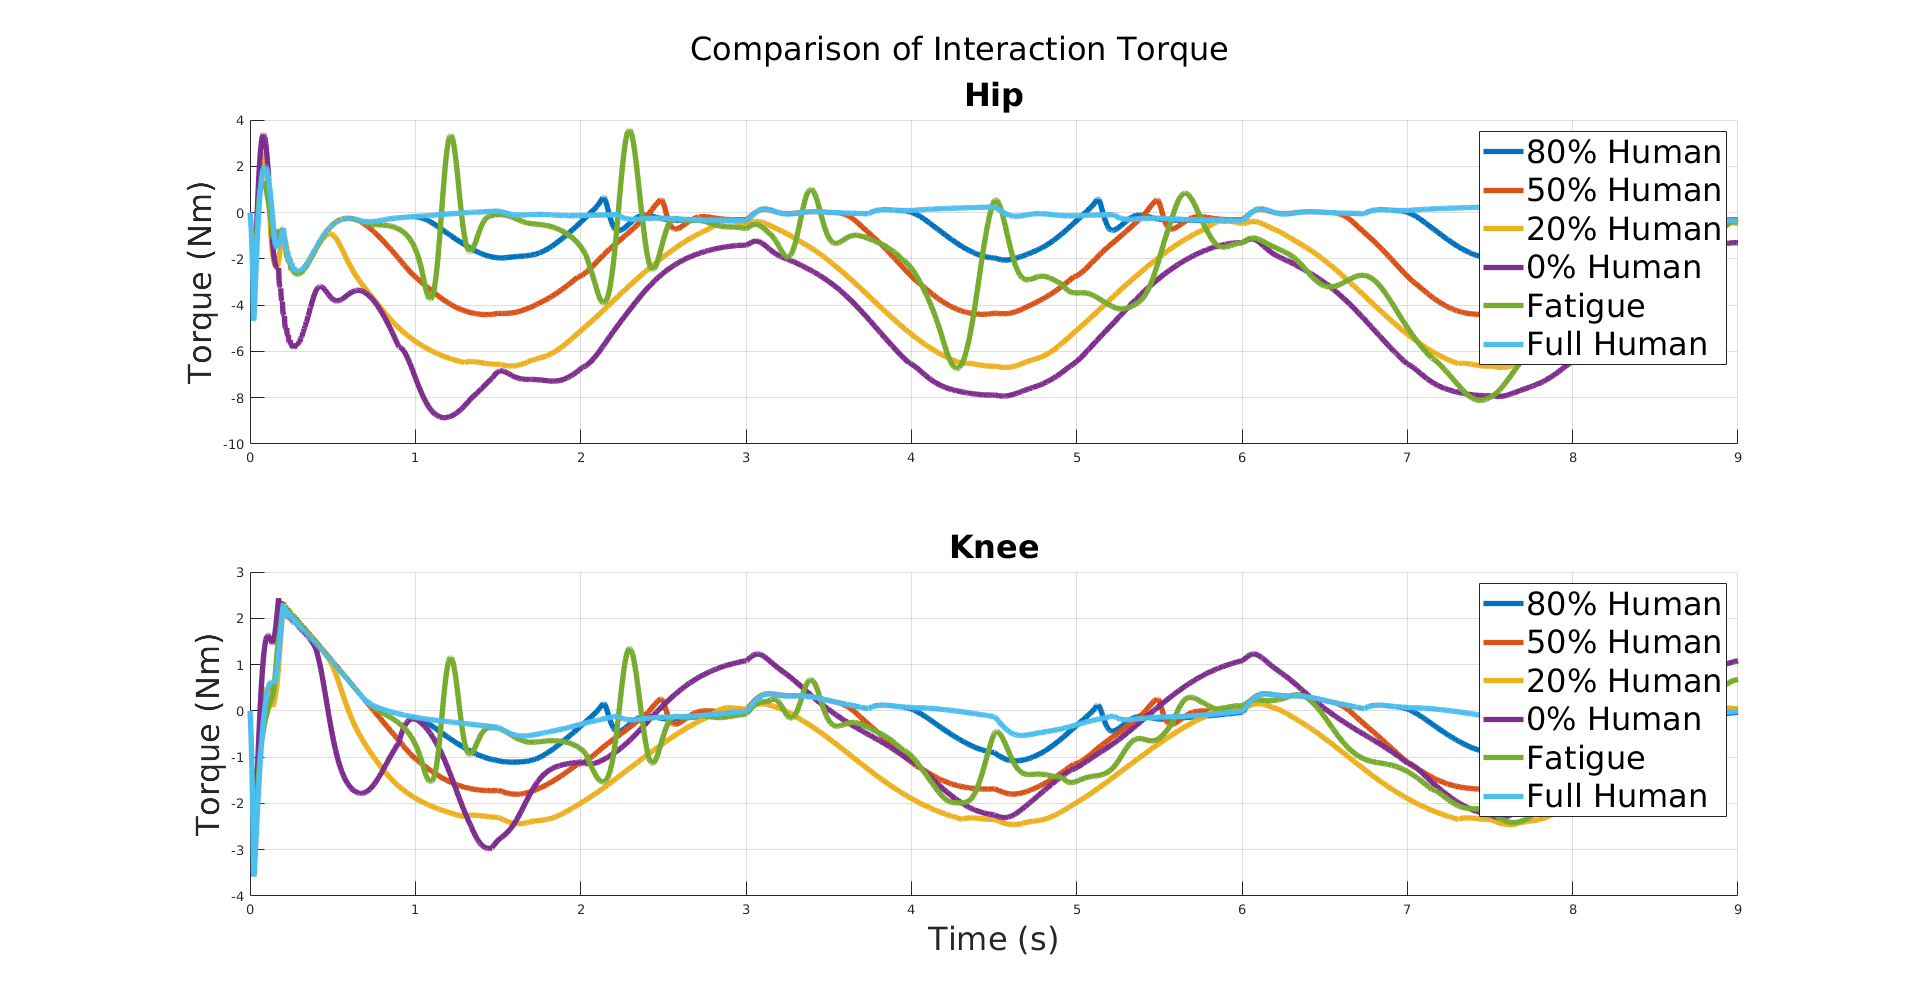
\includegraphics[width=\columnwidth]{images/controllers/trajs/interactions.png}
    \caption[Triple Trajectory Interaction Torques]{Triple Trajectory Interaction Torques}
    \label{fig:InteractionTripleTraj}
\end{figure}


\subsection{Application of Tuning Methodology to Follow a Gait Cycle}


Using the parameters calculated above the model was then used to follow a three gait cycle to observer the steady state motion of the controller. The trajectory was auto generated by combining three gait cycles.  One of the important changes to the model was the using the torques pre-calculated  by the iLQR method (see \autoref{sec:ilqr}) as the standard interaction torques.  This is instead of using a inverse dynamic model since the iLQR controller should produce optimal torques to follow the gait trajectory. The A-SMC then compensates for the disturbances in the system. \autoref{fig:CoopSimulink} shows the Simulink model used to control the gait following model. The outputs torques that are highlighted go to dynamics server which double integrates the output to get the joint positions and velocity. Which are then feedback as the input joint states. The interaction dynamics are the spring-dampener equations which calculate the coupled forces.  



\begin{figure}[h!]
    \centering
    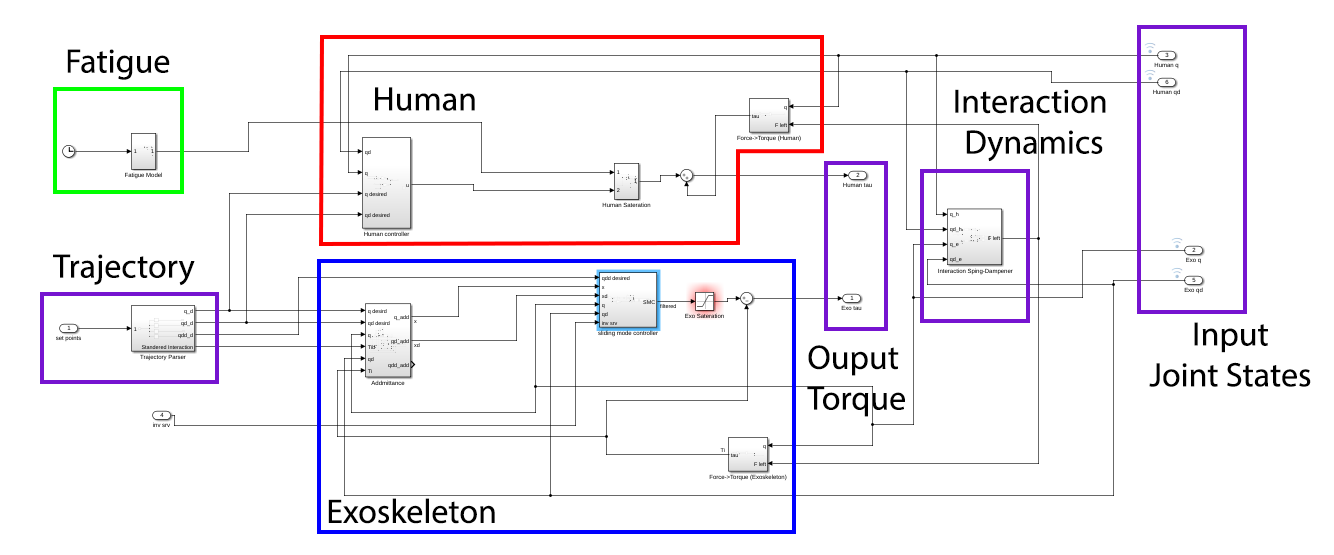
\includegraphics[width=\columnwidth]{images/controllers/upper_model_simulink_edit.png}
    \caption[Simulink Model Cooperative Controller]{Simulink Model of the Cooperative Gait Controller }
    \label{fig:CoopSimulink}
\end{figure}


\author{fig:TripleGaitMotion} shows gait motion with varying human engagement levels. The SMC controller was able to compensate the for the lack of human involvement and track the gait cycle which is more complex then the previous simple trajectory. The initial start of the controller varies slightly however it converges to a steady state operation and track the other gait cycles closely. 

\begin{figure}
    \centering
    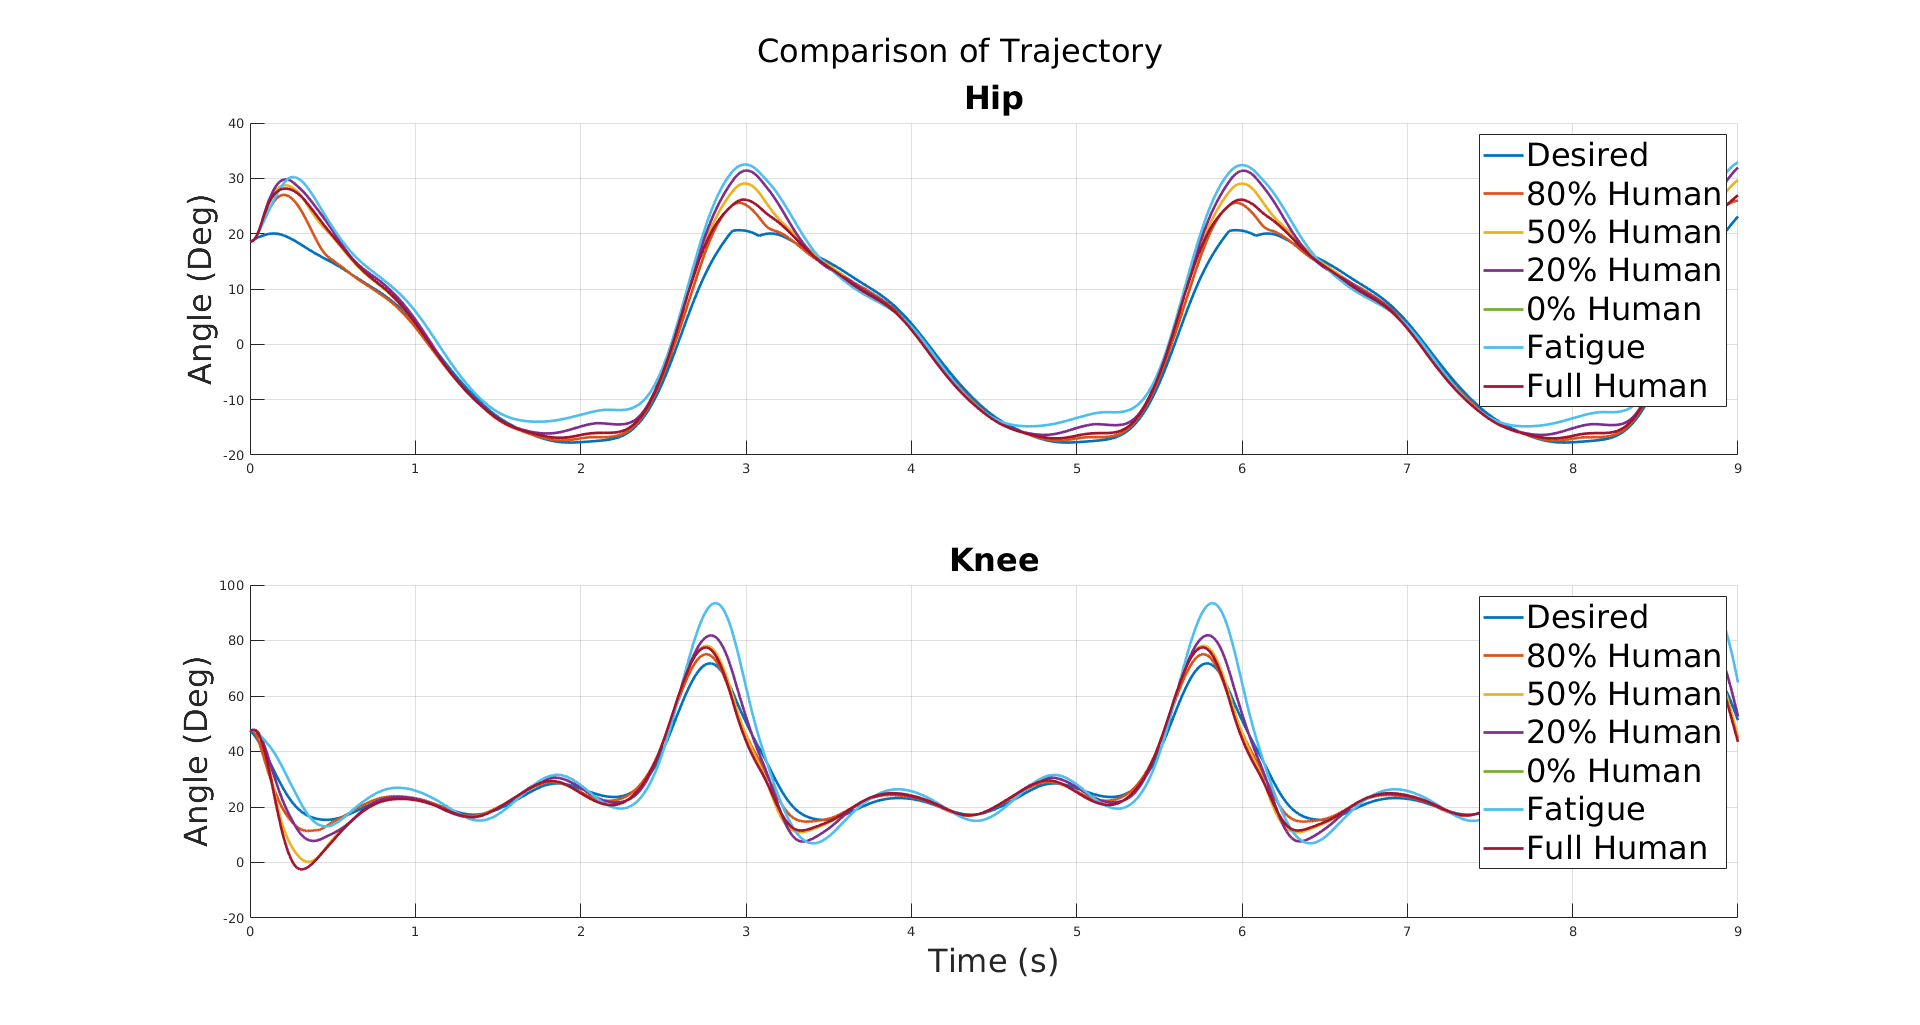
\includegraphics[width=\columnwidth]{images/controllers/gait/traj.png}
    \caption{Triple Gait Cycle}
    \label{fig:TripleGaitMotion}
\end{figure}



\autoref{fig:TorqueOverGaitCycles} shows the torques generated to follow the gait cycles. \autoref{fig:HumanTripleGaitMotion} shows the human torques over the gait cycle. The maximum torque is capped at the different levels. This can been seen where the the torque does not surpass the maximum activation level. The same fatigue profile shown in \autoref{fig:fatprofile} was used to simulate the muscle fatigue. \autoref{fig:SMCTripleGaitMotion} shows the SMC controller torques generated over the gait cycle. \autoref{fig:InteractionTripleGaitInteration} shows the interaction torques between the human and LARRE. Unlike in the simple trajectory model the human torque profile shown here spikes to the saturation limit. The SMC controller torque contain a similar profiles that were observed in the simple trajectory where as the human torque decrees the SMC troque increases. Additional the controller was able to compensate for the time varying fatigue, which is critical for operation where the user may not be able to maintain the required torque through the gait cycle. 

\begin{figure}
    \centering
    \begin{subfigure}{0.8\linewidth}
        \centering
        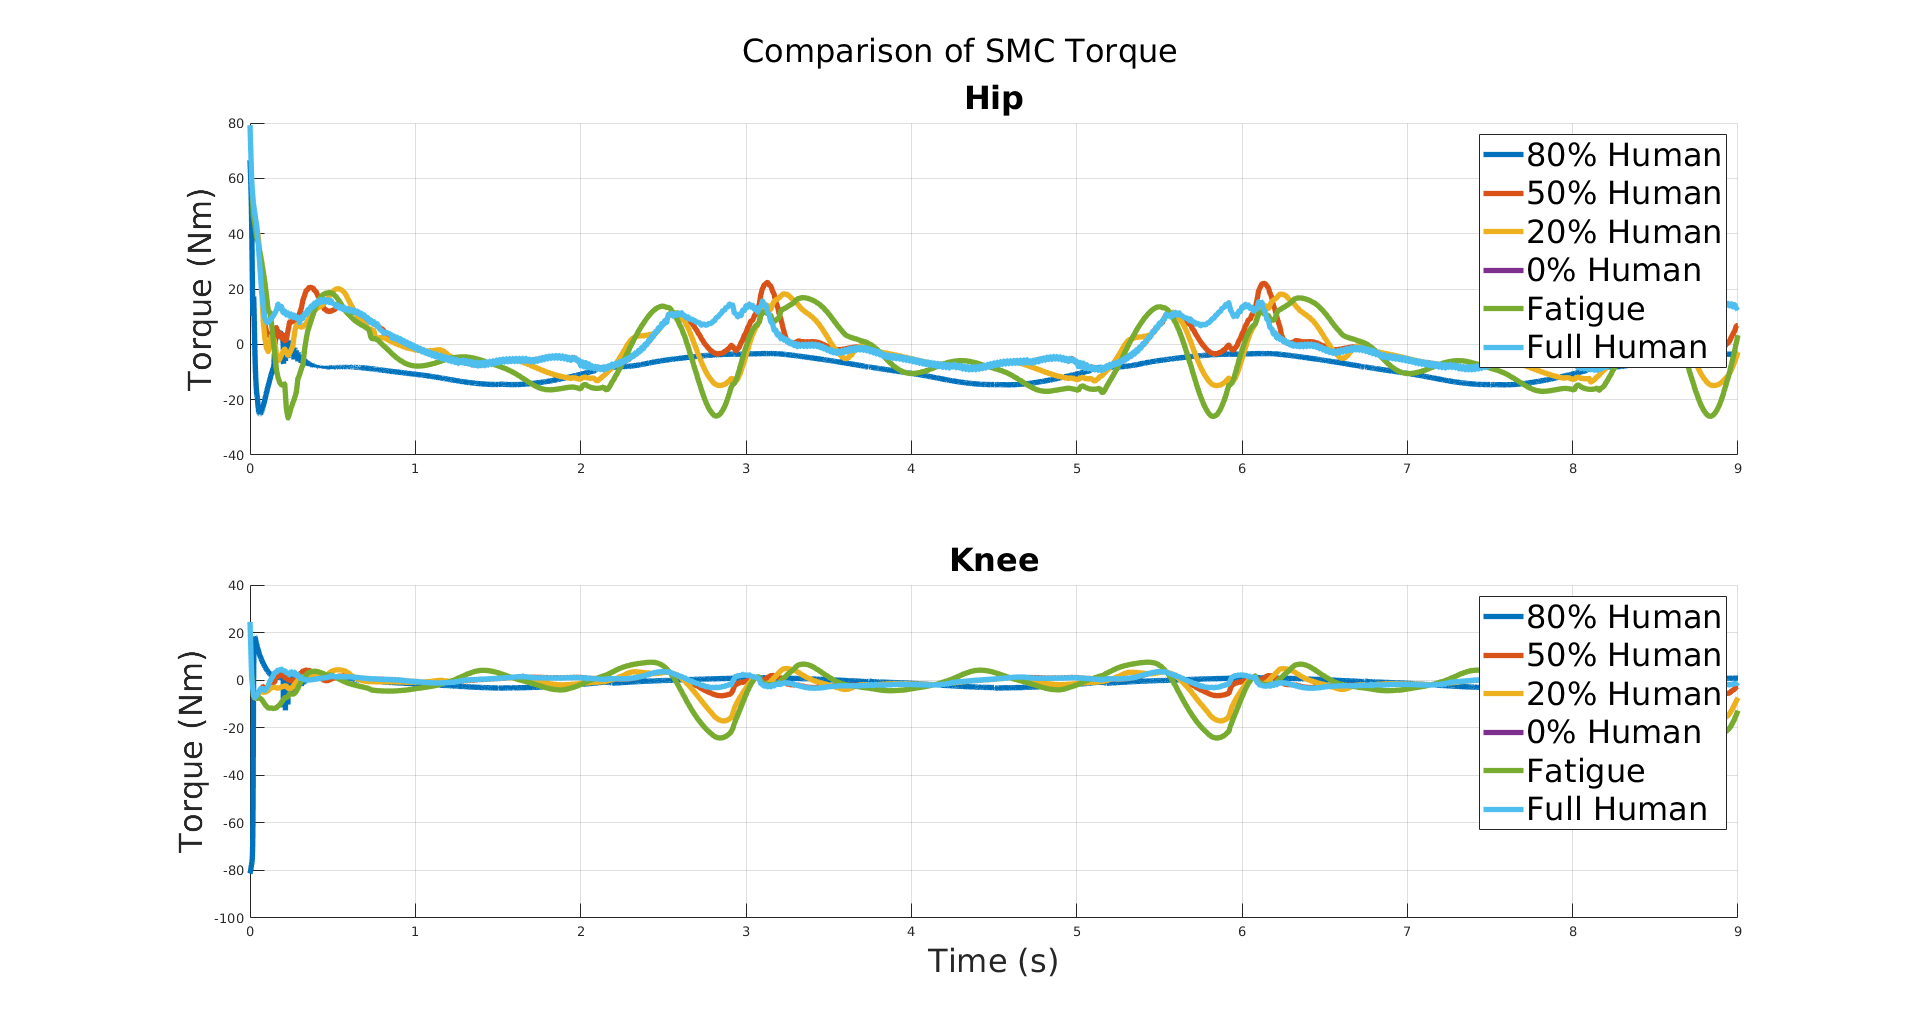
\includegraphics[width=\columnwidth]{images/controllers/gait/SMC.png}
        \caption[SMC Torque Over Gait Cycles]{SMC Torque Over Gait Cycles}
        \label{fig:SMCTripleGaitMotion}
    \end{subfigure}
    \begin{subfigure}{0.8\linewidth}
        \centering
        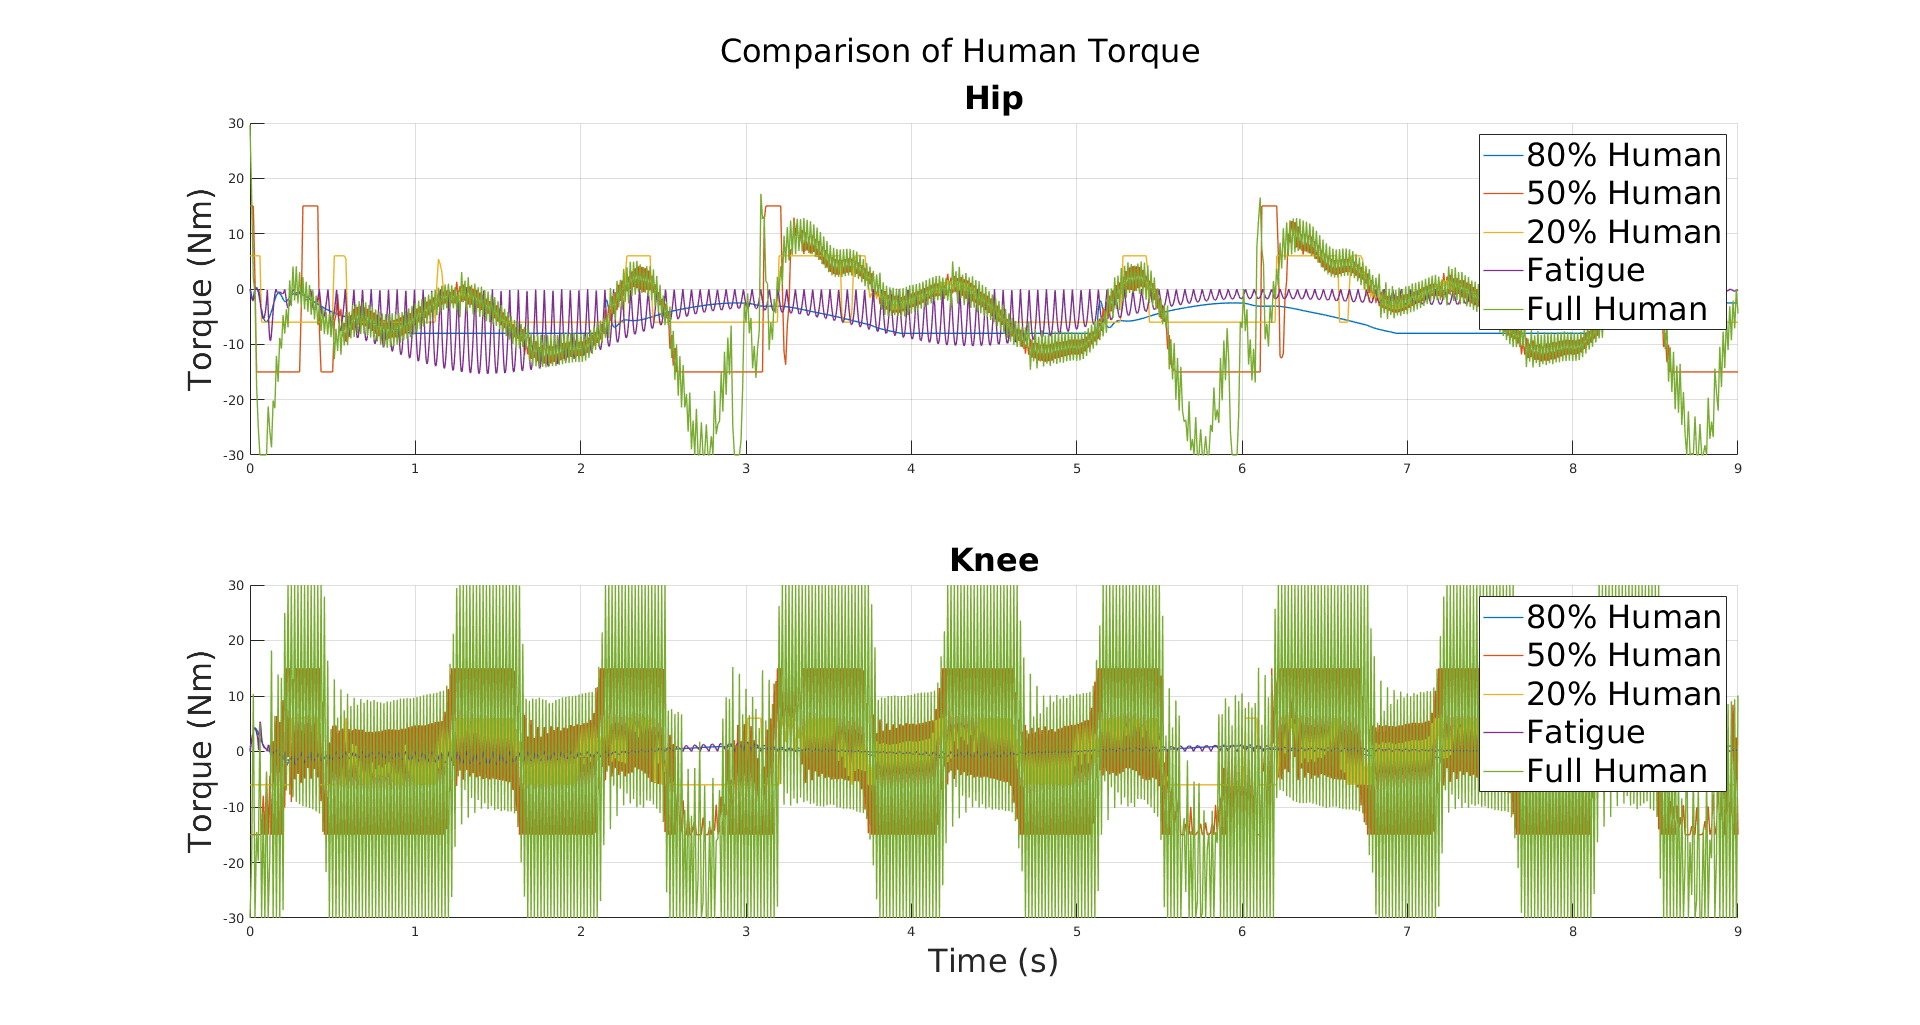
\includegraphics[width=\columnwidth]{images/controllers/gait/human.png}
        \caption[Human Torque Over Gait Cycles]{Human Torque Over Gait Cycles}
        \label{fig:HumanTripleGaitMotion}
    \end{subfigure}
        \begin{subfigure}{0.8\linewidth}
        \centering
        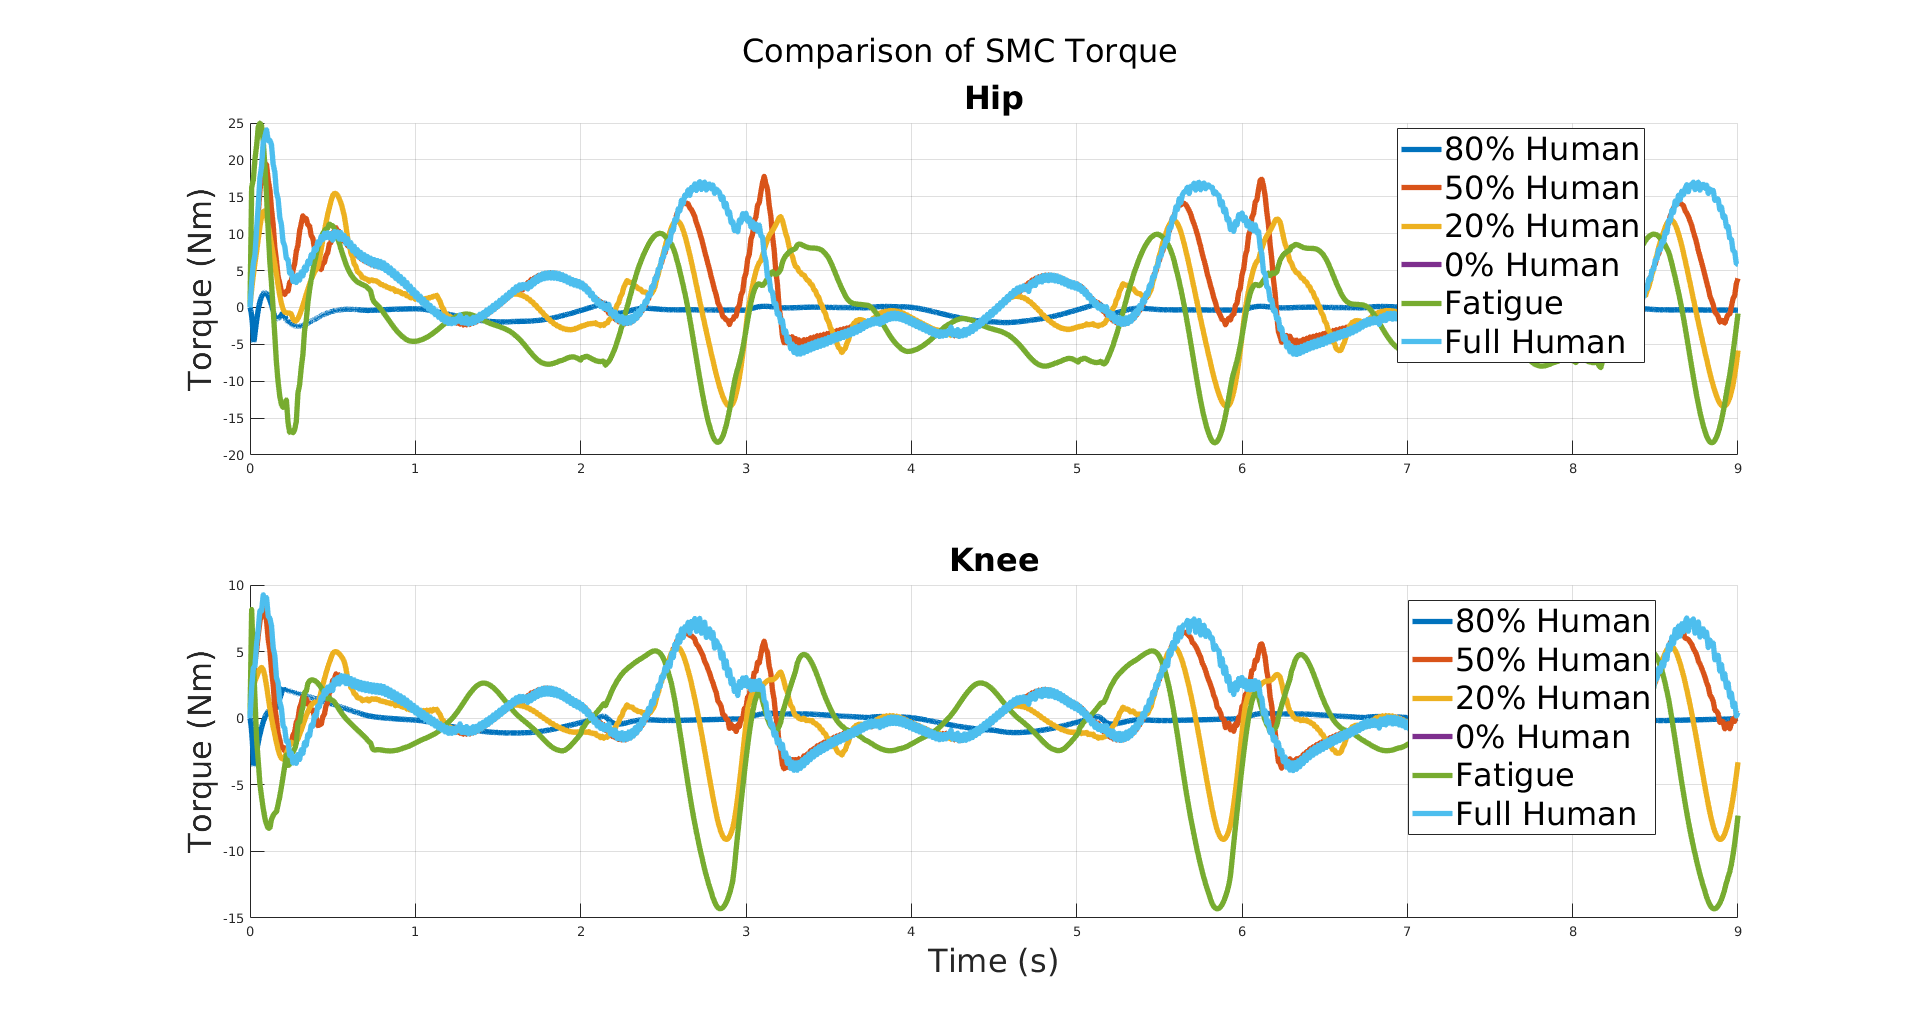
\includegraphics[width=\columnwidth]{images/controllers/gait/feedback.png}
        \caption[Human Torque Over Gait Cycles]{Human Torque Over Gait Cycles}
        \label{fig:InteractionTripleGaitInteration}
    \end{subfigure}
    \caption{Torque Over Gait Cycles}
    \label{fig:TorqueOverGaitCycles}
\end{figure}




\subsection{Complication of ROS-Simulink Integration}

The bridge connecting ROS to Simulink seems to be built assuming that a virtual machine (VM) runs Linux with the host computer running either Windows or OSX. There are built-in tools to set a connect and use a remote host for ROS. This allows for connection to deploy the node to a robot or allows for development on a non-Linux OS. When are remote host is selected (i.e. not using local host) the Simulink node compiled to the catkin\_ws on the VM. 

A bug in the ROS-Simulink framework was discovered during development. While MATLAB as a process of integrating and using custom message in Simulink, it has a bug where is will only build and compile when you set up a VM to be the ROS master and compile to that VM. This also means that the VM catkin\_ws needs a full copy of all the relevant packages and decencies. This bugs was reported to MathWorks\footnote{https://www.mathworks.com/}, who are now fully aware of the bug and are working on a patch for a future release. While it is possible to set up such a pipeline adding a VM into the system significantly complicate the pipeline and add uncertainly into the timing of the controller performs. 


% \subsection{Application of Tuning Methodology}

% The tuning methodology developed for the simplified was applied to tune the cooperative controller for the LARRE. A Simulink model was built with ROS communication to tune the parameters. A model was built to calculate the forward and inverse dynamics on the fly using the \textit{ambf\_control\_system} package. Since this framework used the same AMBF simulation model, it is a good representation of the dynamics.   



% \subsection{Tuning of LARRE controller}

% The above method was then to tune the controller for LARRE. The model dynamics were calculated using the \textit{ambf\_control\_system} package for both the inverse and forward dynamics, allowing the system's response to be estimated on an identical model to the AMBF model but without the need to run AMBF, which would complicate the learning process. This was accomplished using the built-in ROS-Simulink bridge. 

% The tuning was done on a Ryzen$\texttrademark$ 5900x\footnote{https://www.amd.com/en/products/cpu/amd-ryzen-9-5900x} with $32Gb$ of memory and a Nvidia$\texttrademark$ 2700S GPU\footnote{https://www.nvidia.com/en-us/geforce/graphics-cards/rtx-2070-super/}. Due to many parameters (74 parameters assume that matrix elements off the diagonal are 0), the tuning process had to be done in batches.  If too many iterations were attempted, the computer would run out of memory running, causing the computer to crash. To solve this problem, only five iterations at a time then restarting the process with the final parameters of an iteration being the initial parameters of the next run. 




% \autoref{fig:coopCost} Show the converges of the response optimization. For systems with many parameters, upper and lower bound must be defined; this helps bound the search space and reduce optimization time. While the upper bound is hard to determine, the lower bound is known to be greater than 0, the $\beta$ parameter is bound between $0$ and $1$. It is also important to ensure the off-diagonal of the matrix is strictly 0 since only the diagonal elements are required. \autoref{fig:coopParams} shows how the parameters changed over the iterations. Twice the number of iterations is displayed because two resets were allowed in the optimization. They are split into different graphs since the parameters of different magnitudes and this allows for values to be better displayed. While it is difficult to determine how the parameters affect the overall model, all the parameters are correlated, and the system is highly non-linear. However, we can see that the magnitude of the parameters is critical. While the parameters did vary over time, they did not change magnitude.  


% \begin{figure}[h]
%     \centering
%     \begin{subfigure}{\textwidth}
%         \centering
%         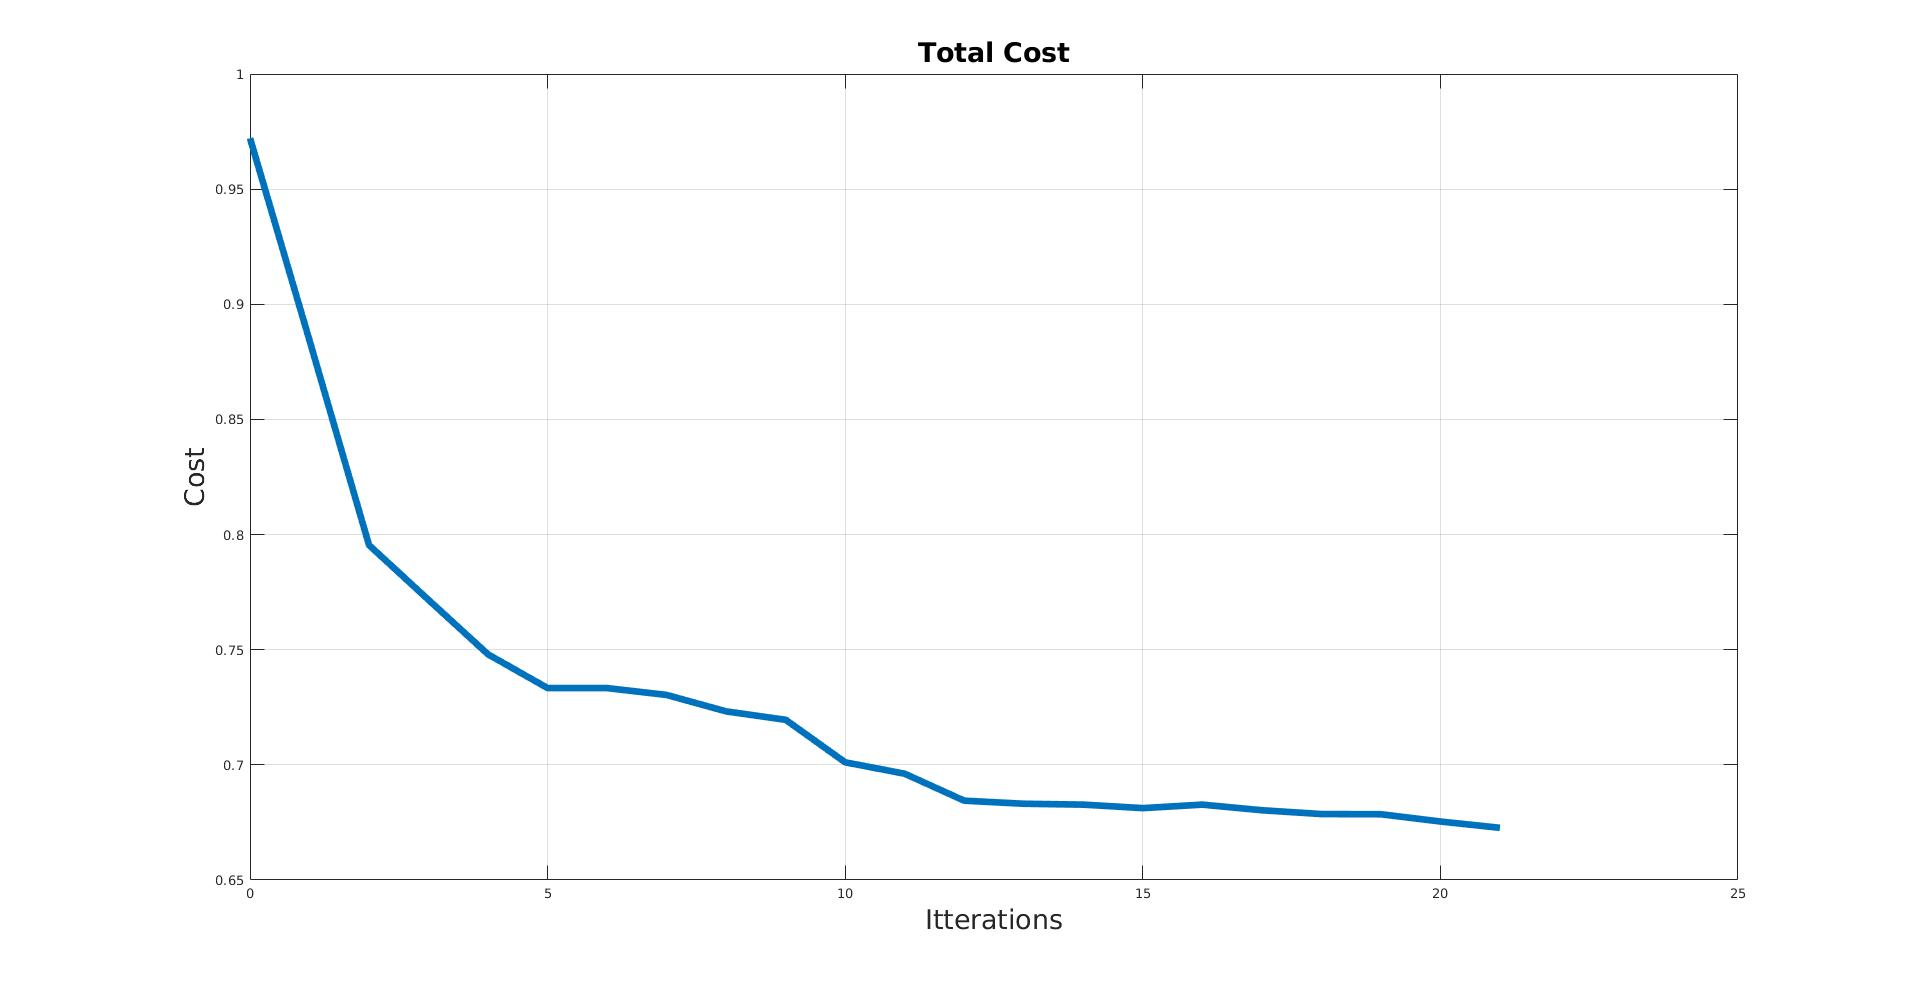
\includegraphics[width=\linewidth]{images/controllers/coop_cost.jpg}
%         \caption[Cost for LARRE Controller]{Cost of tuning the LARRE controller.}
%         \label{fig:coopCost}
%     \end{subfigure}
%     \begin{subfigure}{\textwidth}
%         \centering
%         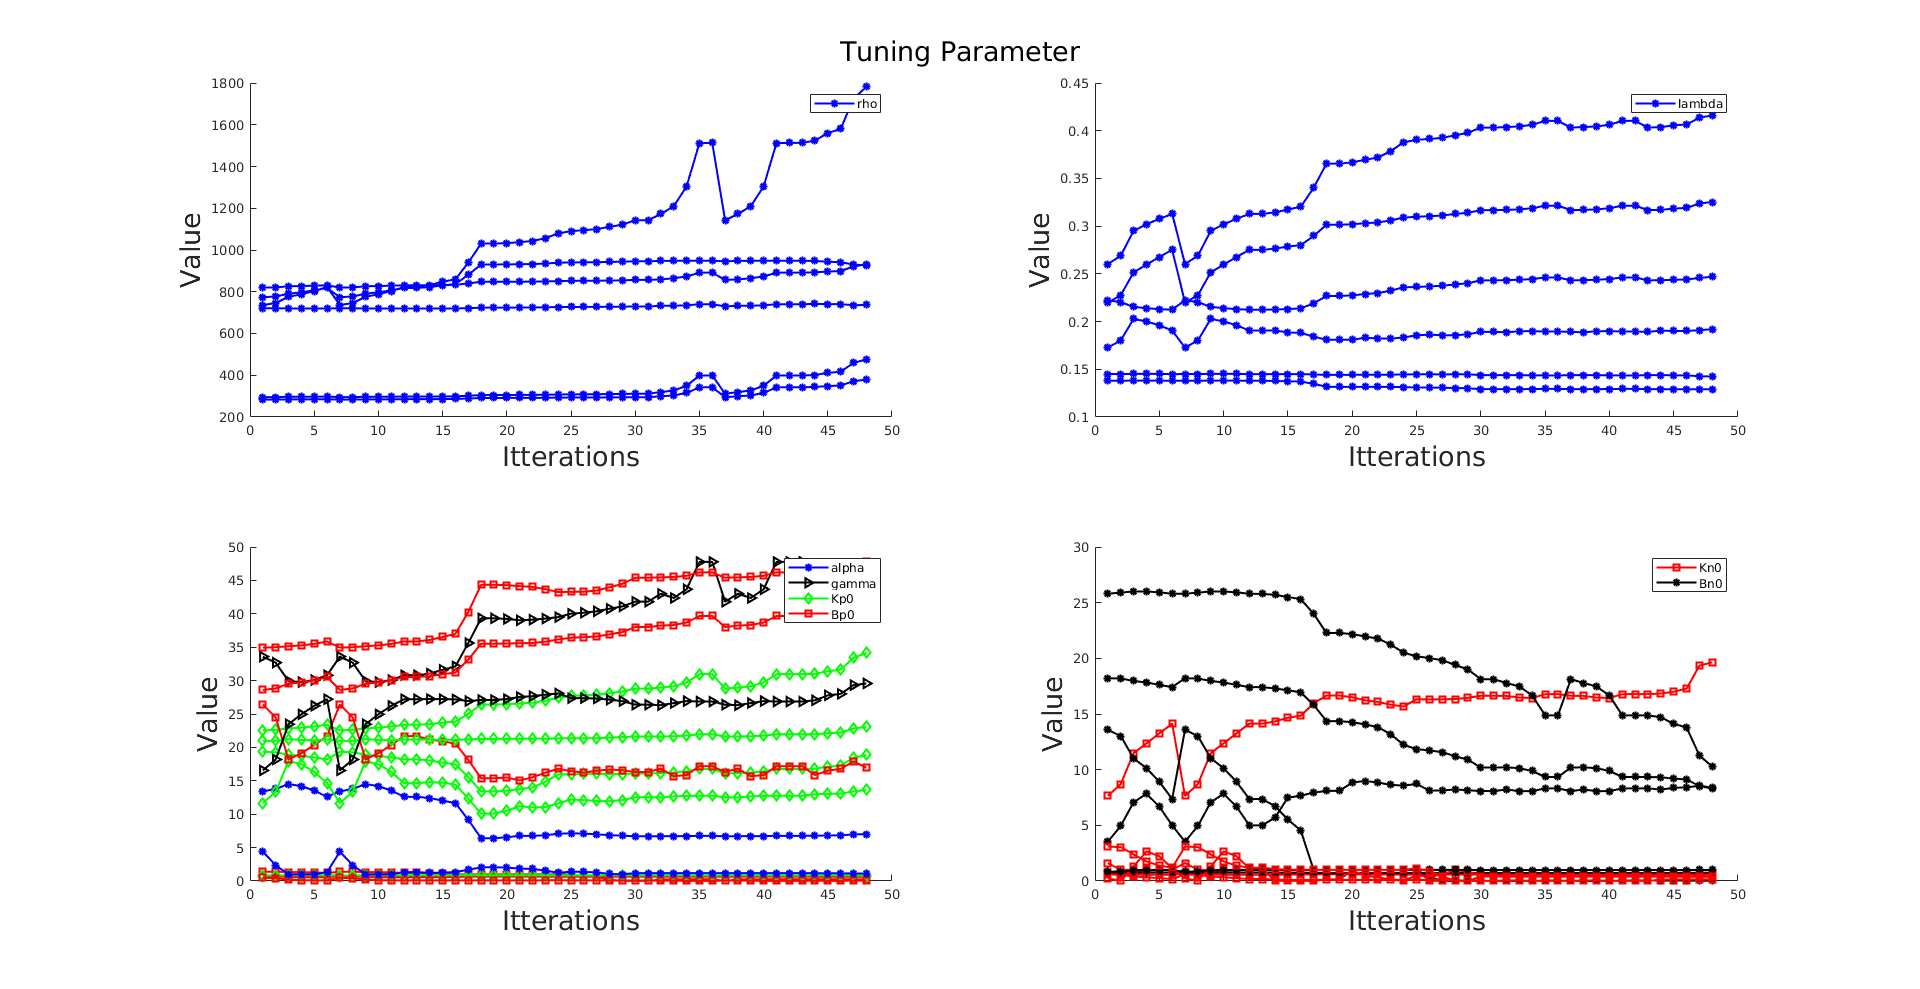
\includegraphics[width=\linewidth]{images/controllers/all_params.png}
%         \caption[Double Pendulum: Positive Alignment-Trajectory]{Trajectories of double pendulum}
%         \label{fig:coopParams}
%     \end{subfigure}
%     \caption[Parameter updates for LARRE Controller]{Parameter updates for LARRE Controller.}
%     \label{fig:coopParams}
% \end{figure}



% \autoref{fig:SMC_connection} shows a high-level overview of the system connections. A virtual machine (VMWare\footnote{https://www.vmware.com/products/workstation-player.html}) was required to run a ROS master due to a bug in the deployment of the Simulink ROS node. The main control system sends set points the Simulink control along with receiving constant state feedback. The Simulink control node calculates the effort and sends it back to the main controller, which sends it down to AMBF. Additionally, the \textit{ambf\_control\_system} is used to calculate the inverse dynamics of the model.   

% \begin{figure}
%     \centering
%     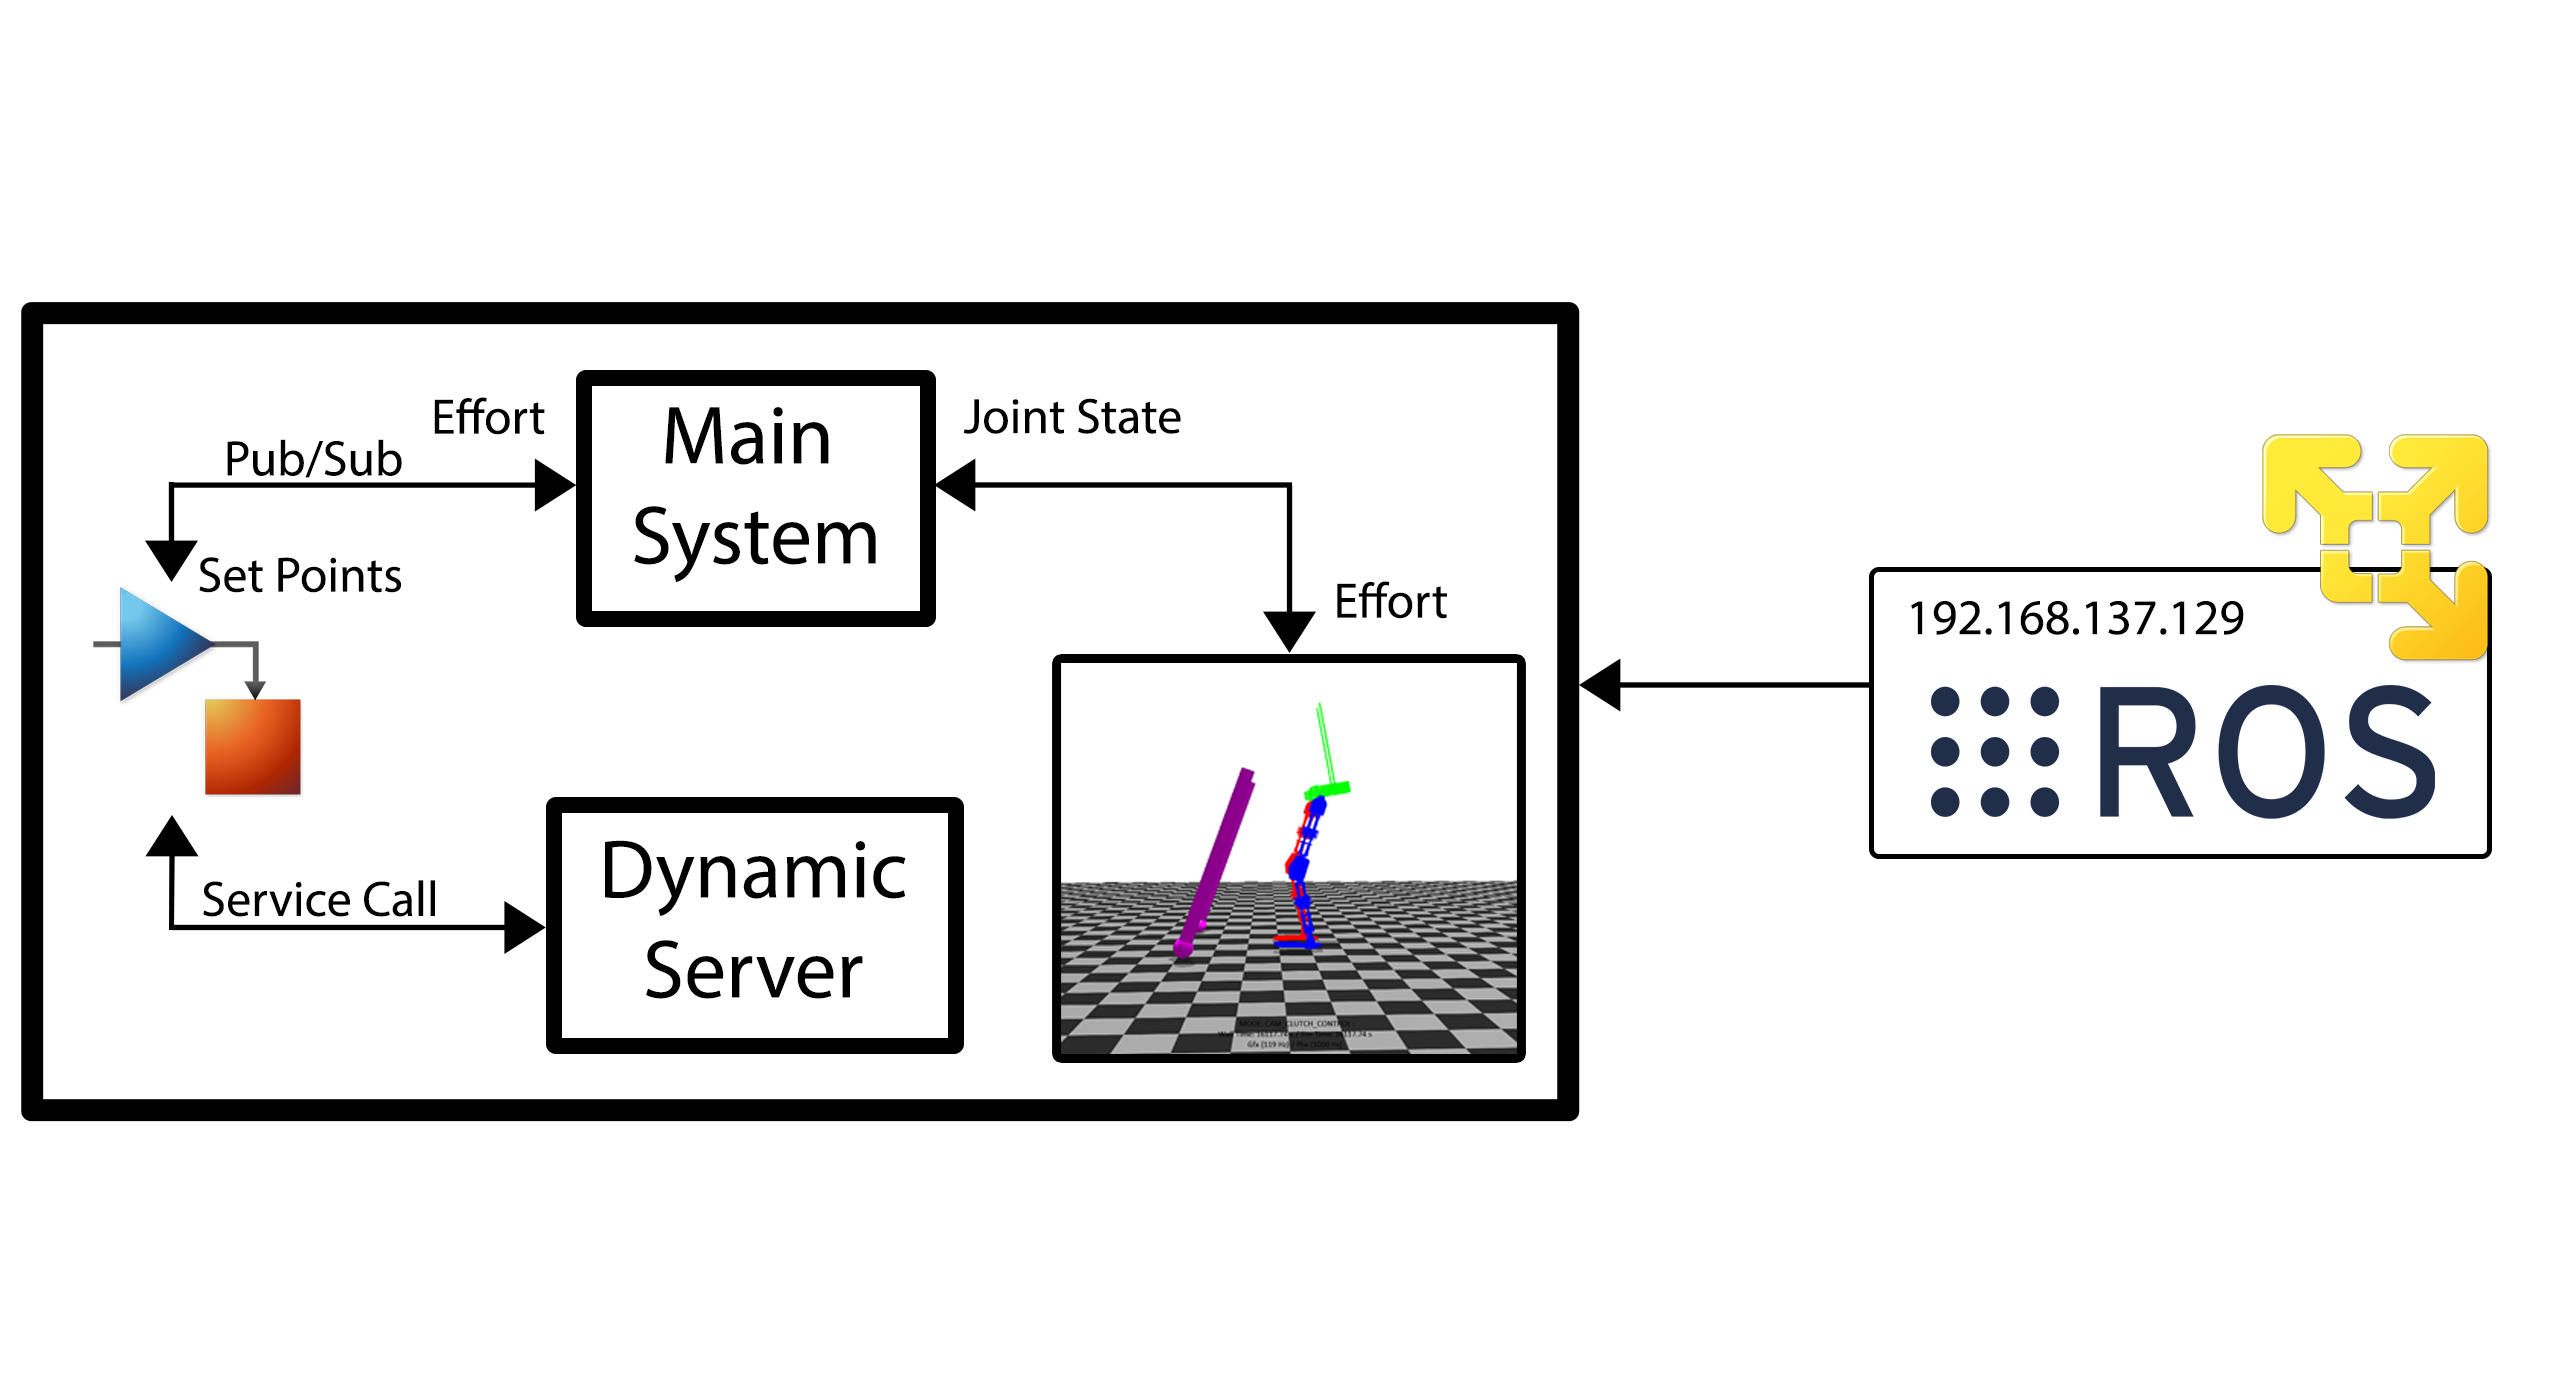
\includegraphics[width=\textwidth]{images/controllers/simulink_connection.png}
%     \caption[SMC Connection Overview]{SMC Connection Overview.}
%     \label{fig:SMC_connection}
% \end{figure}


% The sliding surfaces are shown in \autoref{fig:simple_statespace}. The graphs are shown for the hip, knee, and ankle. The graphs are now as smooth as the simple double pendulum model graphs and converge slightly before reaching 0. This can be repeating the optimization method described above until more optimal parameters are calculated. This can also be used to solve the slight bend in all the graphs.  

% \begin{figure}
%     \centering
%     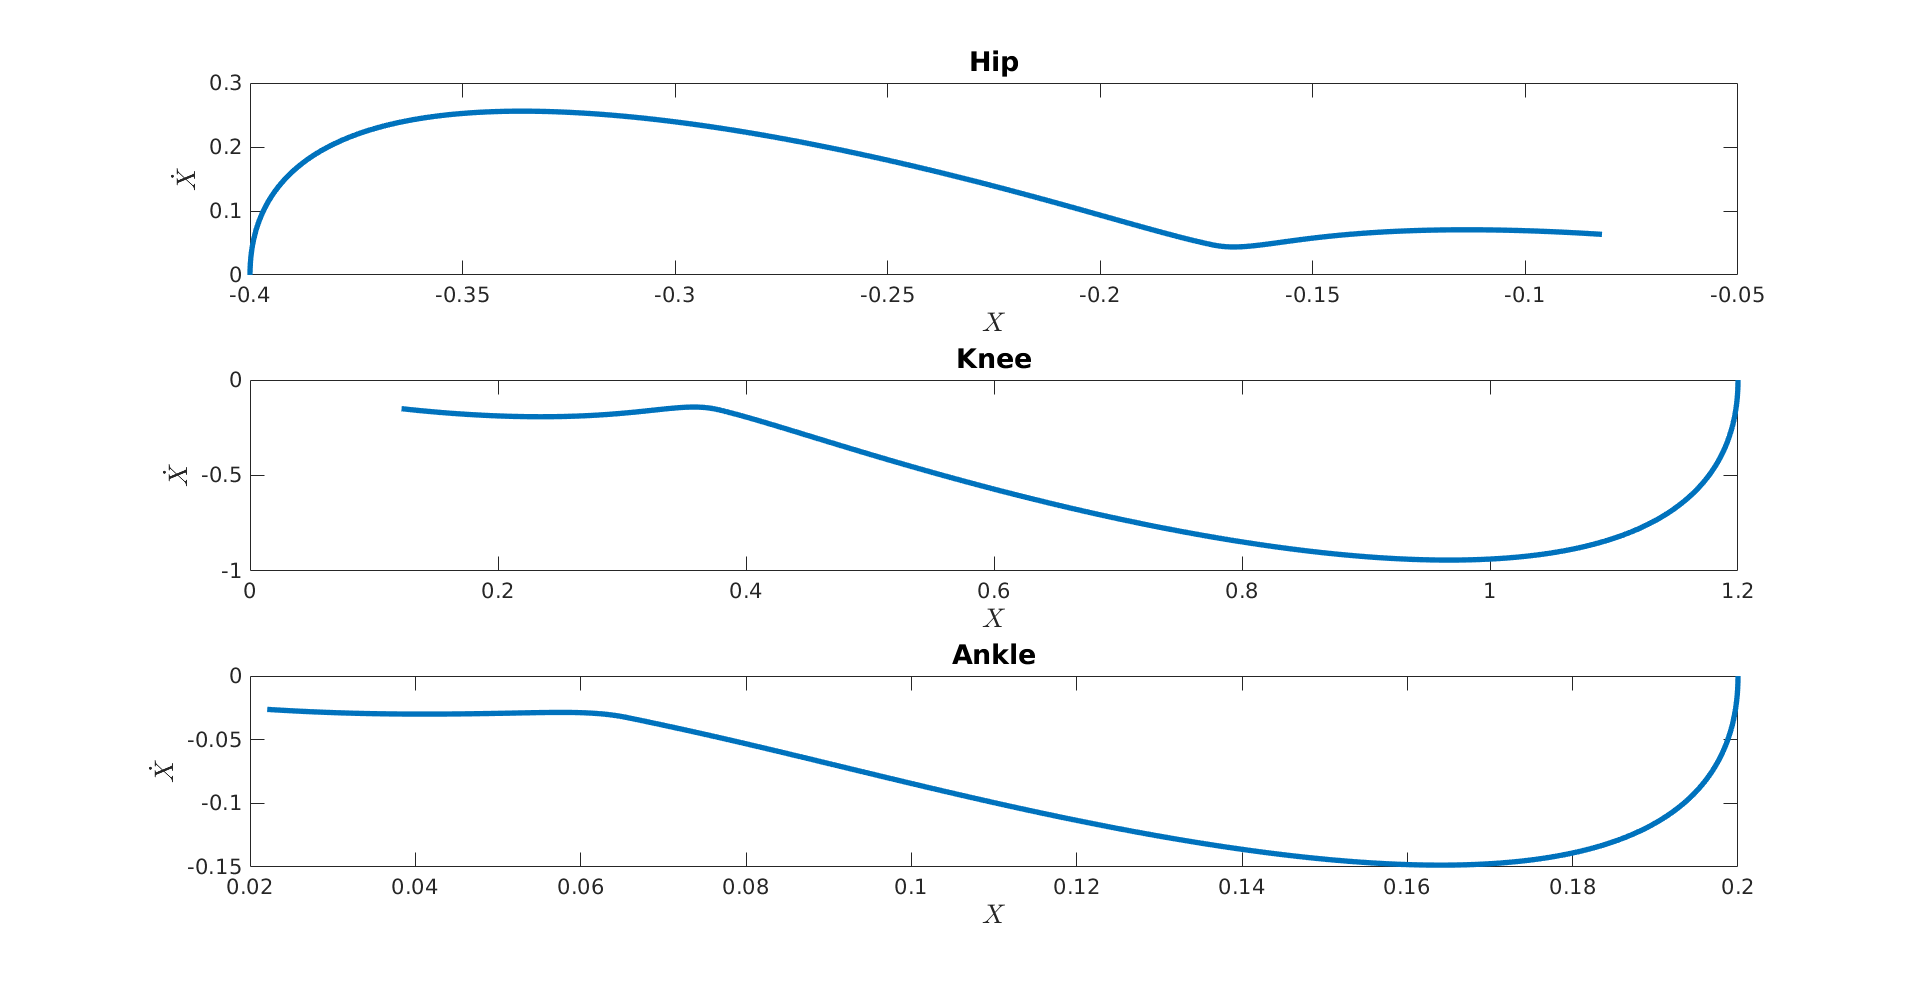
\includegraphics[width=\textwidth]{images/controllers/statespace_simple.png}
%     \caption[Controller State Space]{Controller state space graphs}
%     \label{fig:simple_statespace}
% \end{figure}


% \subsection{Complication of ROS-Simulink Integration}

% The bridge connecting ROS to Simulink seems to be built assuming that a virtual machine (VM) runs Linux with the host computer running either Windows or OSX. There are built-in tools to set a connect and use a remote host for ROS. This allows for connection to deploy the node to a robot or allows for development on a non-Linux OS. When are remote host is selected (i.e. not using local host) the Simulink node compiled to the catkin\_ws on the VM. 

% A bug in the ROS-Simulink framework was discovered during development. While MATLAB as a process of integrating and using custom message in Simulink, it has a bug where is will only build and compile when you set up a VM to be the ROS master and compile to that VM. It does work when you just use the \textit{Play} method; however, this is an order of magnitude slower as shown in \autoref{fig:SimulinkTimingComparison}. By building and compiling the controller into a ROS node as a lower mean and variance than just playing the model. This is important since if the controller runs too slowly and the timing is inconsistent, the controller will not perform properly. This also means that the VM catkin\_ws needs a full copy of all the relevant packages and decencies. This bugs was reported to MathWorks\footnote{https://www.mathworks.com/}, who are now fully aware of the bug and are working on a patch for a future release. 


% \begin{figure}
%     \centering
%     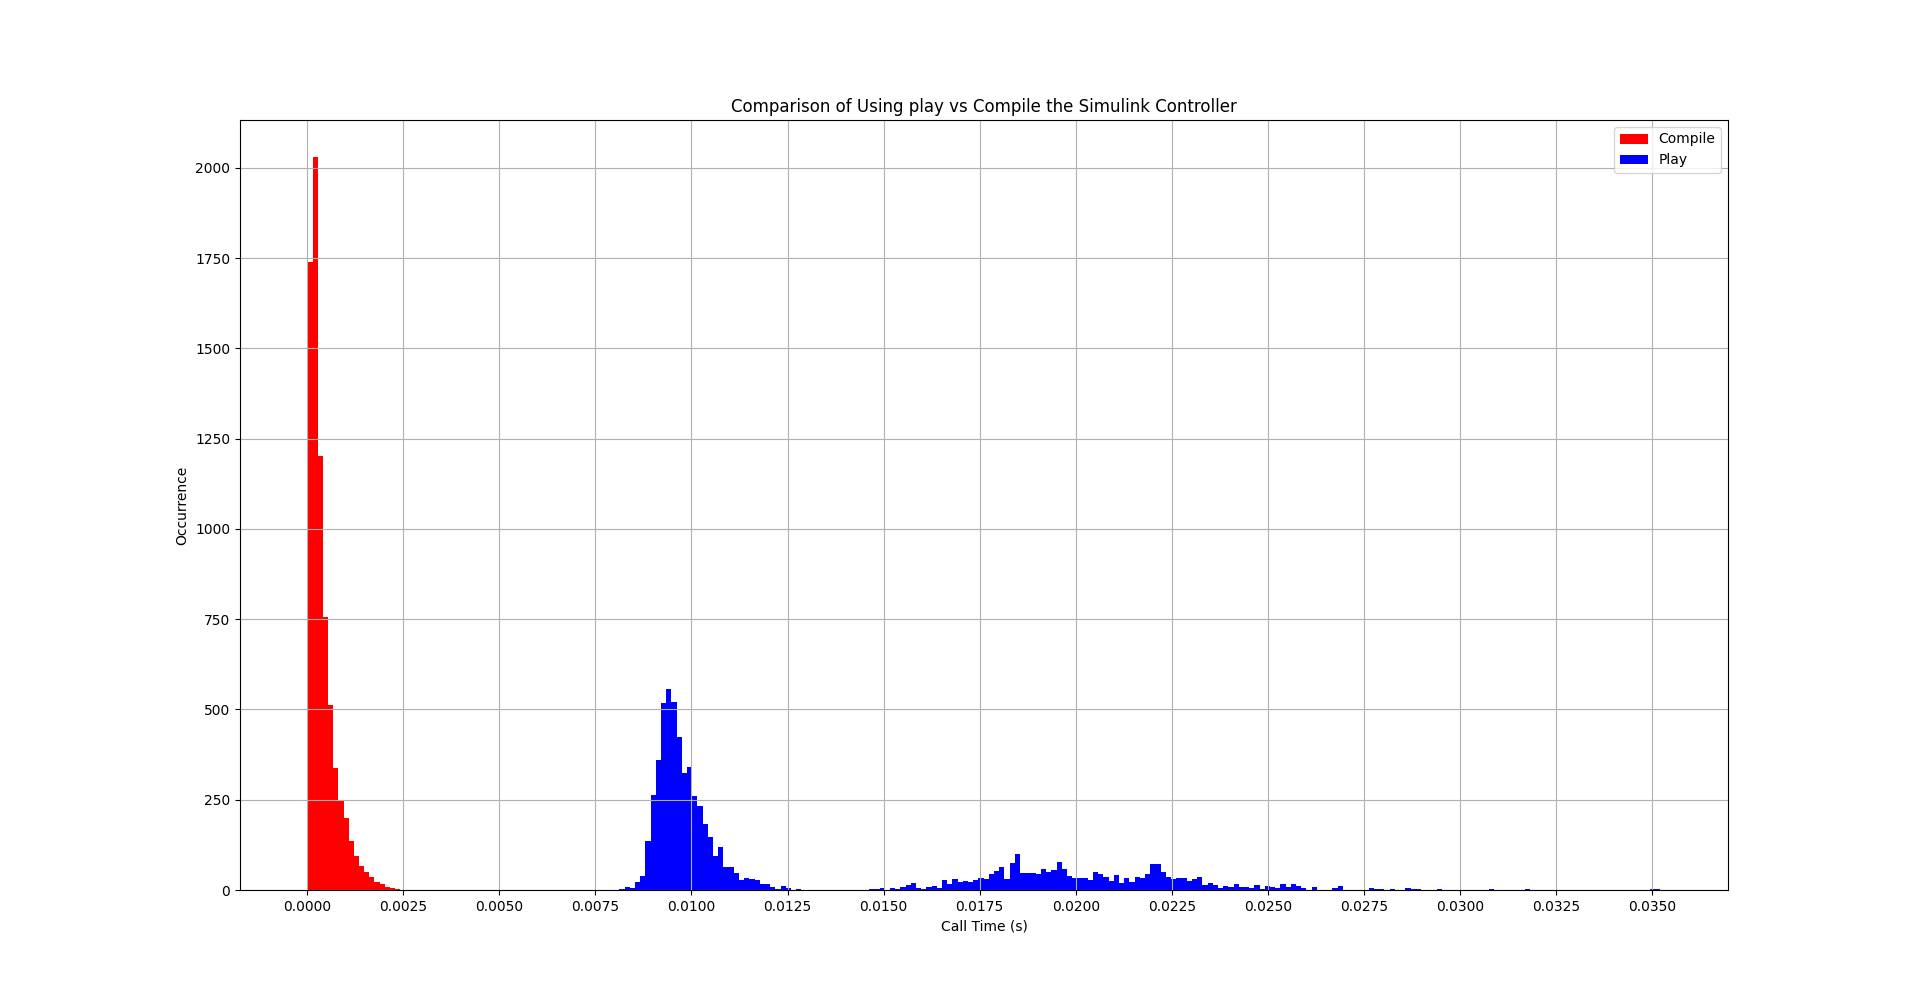
\includegraphics[scale=0.35]{images/controllers/timing_comparison.png}
%     \caption[Simulink Timing Comparison]{Timing Comparison of using the \textit{Build and Run} vs \textit{Play} method}
%     \label{fig:SimulinkTimingComparison}
% \end{figure}

% Additionally, another problem was with the ROS-Simulink communication, which caused the MATLAB to lose track of message definitions and enter an inescapable loop that seized the OS's focus and corrupted the matlabpref file. This problem could only be solved by hard rebooting the computer. Once the computer was rebooted, the \textit{matlabpref} had to be deleted, and all the custom ROS message files had to be re-linked. The cause of this bug is still unknown.






\section{Validation on Physical System}

The work in this section is still in development. I plan to test the ASMC on the system by having the assistie system act at different engagement levels. The tests will resemble the tests conducted on the simulated system discussed above. I will measure the position and applied torque to both the assistie and assistor systems and compare the measurements to a simulation of the same model.   


To test the controller,  a simple physical system was developed and built; this simplified system shows how the controller works on a real system.  \autoref{eq:armDyn} show the dynamics equation for a single-arm where $m$ is the mass of the arm and $l$ is the length of the arm. This system consists of two single degrees of arms; where one is the \textit{assistie} arm and the other is the \textit{assistor} arm.

\begin{equation}
    \tau = \frac{4}{3}ml^2 \ddot{\theta} + \frac{1}{2}ml \cos(\theta)
    \caption{Dynamics equation of a single arm of the system}
    \label{eq:armDyn}
\end{equation}

 The arms were connected with a Velcro strap piece of foam between the two arms to prevent the arms from bending inward. Each of the arms weighed approximately $90g$ and $0.3m$ long. An additional $20g$ was added to the \textit{assistie} arm to simulate the human system being heavier than the exoskeleton system. \autoref{fig:phyicalTestingSystem} shows the physical testing system. The arms are controlled by brushed DC motors with feedback from potentiometers for position sensing. A computer running Simulink acts as the high-level controller and a Teensy 4.0 \footnote{https://www.pjrc.com/store/teensy40.html} as the low-level controller communicating over a serial line. The motors are controlled by Performance Motion Digital motor controllers (Performance Motion Devices, Inc., 1 Technology Park Dr, Westford, MA 01886). Each of the motors is controlled by a 75W Atlas driver (MD211048/02VB) through the development board (MDK4LI0000V) (See Appendix C for the motor setup code) . The Teensy board communicates to the drivers over SPI by sending torque commands to each of the drivers, which delivers the proper current commands to the motors. \autoref{fig:phyicalTestingDiagram} shows the connection diagram; the computer is the high-level controller and the Teensy acts as the low-level controller. The controller was able to operate at $500Hz$. 
 



\begin{figure}[h!]
    \centering
    \includegraphics[width=\linewidth]{images/controllers/phyical system.png}
    \caption[Physical A-SMC Testing System]{Physical testing system of two connected arms. A Teensy 4.0 is used as a lower-level controller. Each arm has its own potentiometer and is controlled by a brushed DC motor. The arms are connected by a velcro strap and a piece of foam between the arms prevents the arms from bending inward. The DC motors are controlled by Atlas motor drivers. }
    \label{fig:phyicalTestingSystem}
\end{figure}


\begin{figure}
    \centering
    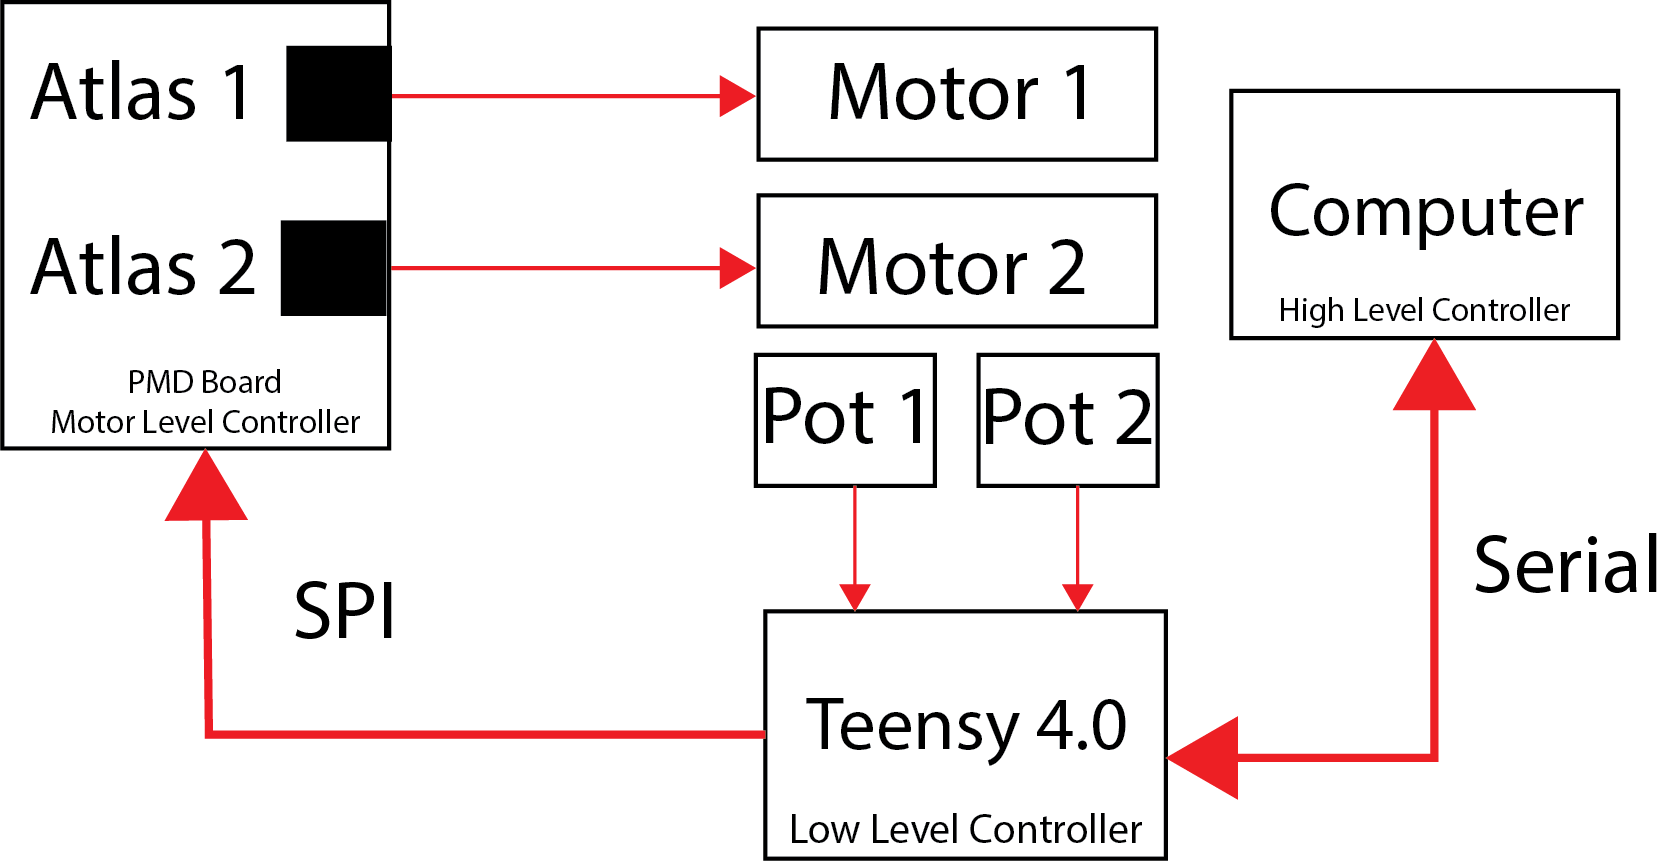
\includegraphics[width=\linewidth]{images/controllers/testing_system_diagam.png}
    \caption[Testing A-SMC System Diagram]{Connection diagram of the testing system. The computer communicates with the Teensy over serial protocol sending shown two torque command and receiving two position. The Teensy uses SPI to communicate with the motor drivers. }
    \label{fig:phyicalTestingDiagram}
\end{figure}


\autoref{fig:phyicalTraj} shows the comparison of the trajectories for both the \textit{assistie} and \textit{assistor} systems both a fully engagement and no engagement systems. The blue line is the desired motion, the red line is the path of the of the \textit{assistie} system with full engagement, the yellow line is the \textit{assistor} system with full engagement, the purple line is the path of the \textit{assistie} system with no engagement, and the green line is the path of the \textit{assistor} system with no engagement. 

The system was able to follow the desired motion when the system was the \textit{assistie} system was able to provide torque and when the A-SMC was fully engaged. \autoref{fig:phyicalTorque} shows the torque profiles for the systems, when the  \textit{assistie} torque was engaged the A-SMC controller was decreased. The blue line is the torque profile when the  \textit{assistie} system is full engaged and the orange line is when then \textit{assistie} system is not engaged. This result shows the the controller can be used on physicals systems. The paths of the  \textit{assistie} and  \textit{assistor} do not perfectly track each other, this is because of the soft connection between the two systems. A more rigid connection could solve this problem but may not accurately represent a real exoskeleton system. The The step like motion of the trajectories is caused by the low update speed and backlash in the motor gearboxes, by increase the control loop frequency a smooth control signal can be generated the will produce a better trajectory. The motors and gearboxes have a considerable about of backlash this causes in accuracy in the system positing and control. By increase and the control rate and using better gearboxes and motors this two problems should be mitigated.  This will also help the A-SMC controller which overshoot the final position of the desired motion slightly, a faster control rate will allow the controller to respond to the motion of the robot. 



\begin{figure}[h!]
    \centering
    \begin{subfigure}{\linewidth}
        \centering
        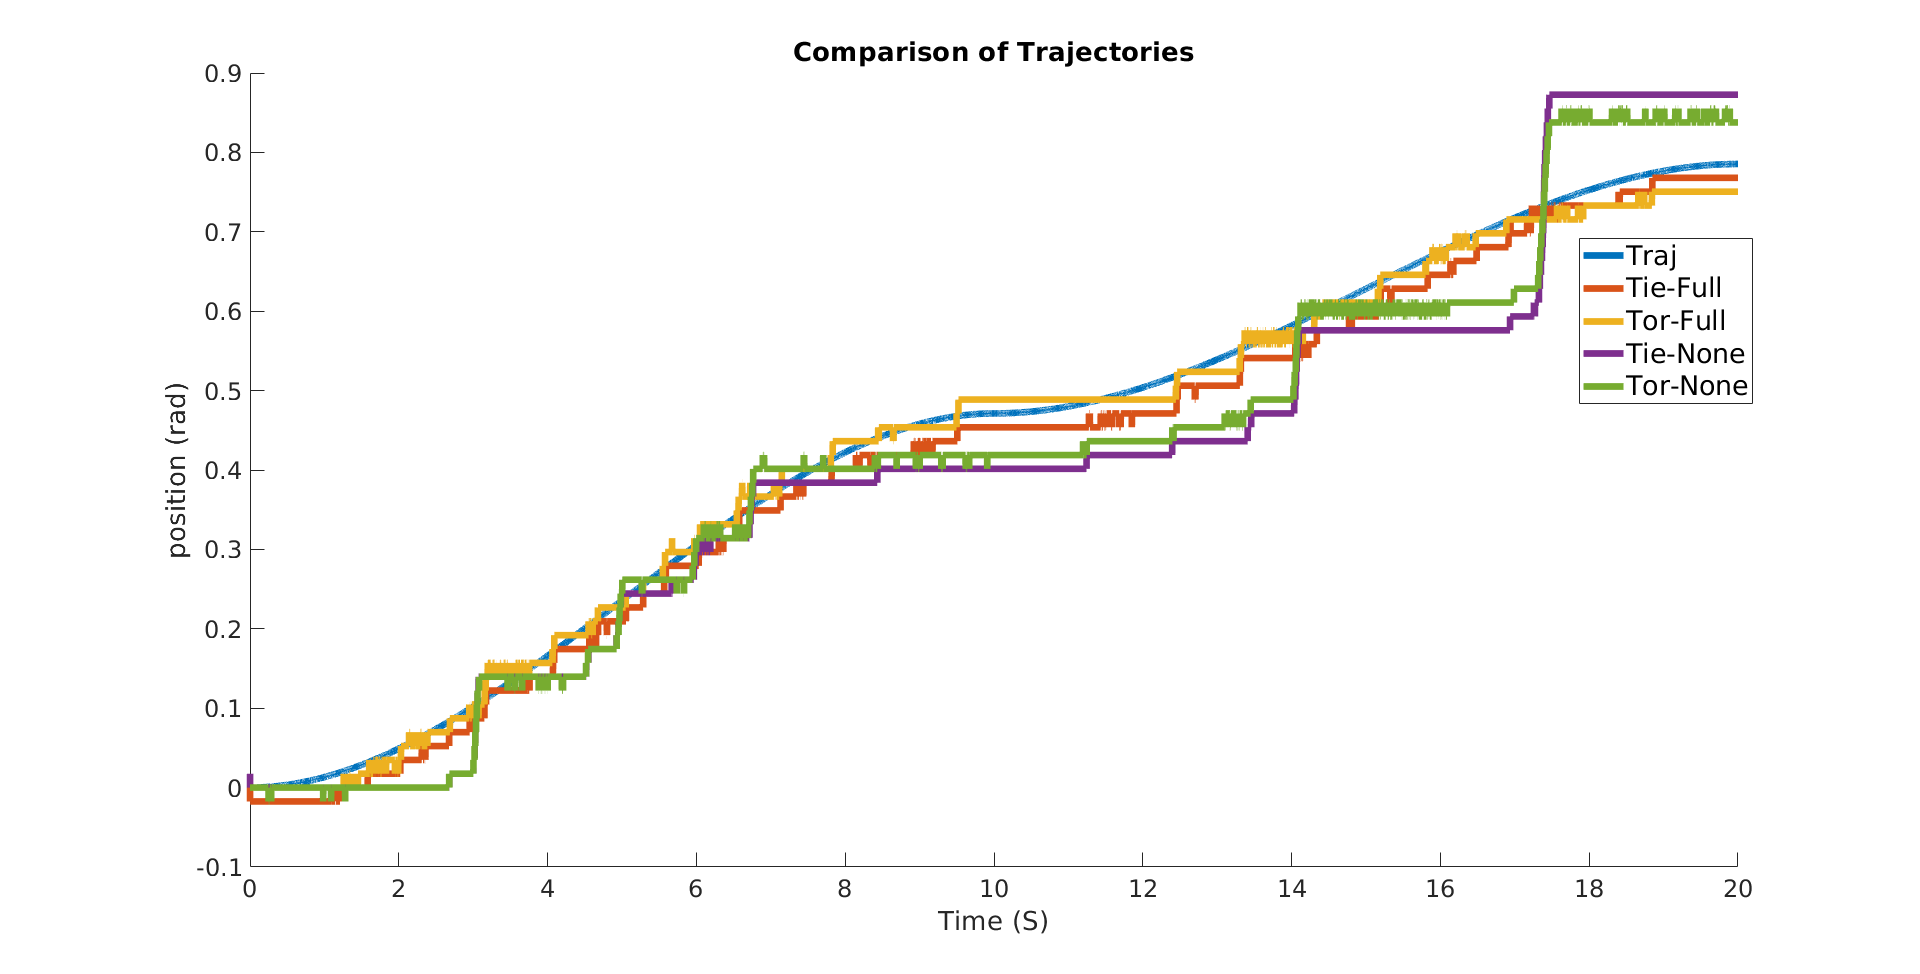
\includegraphics[width=\columnwidth]{images/controllers/comptraj2.png}
        \caption[Physical System Trajectory Tracking]{Comparison of a the trajectory on a physical system. The "None" systems have no engagement from the \textit{assistie} system. The "Full" systems has \textit{assistor} has fully engaged. }
        \label{fig:phyicalTraj}
    \end{subfigure}
        \begin{subfigure}{\linewidth}
        \centering
        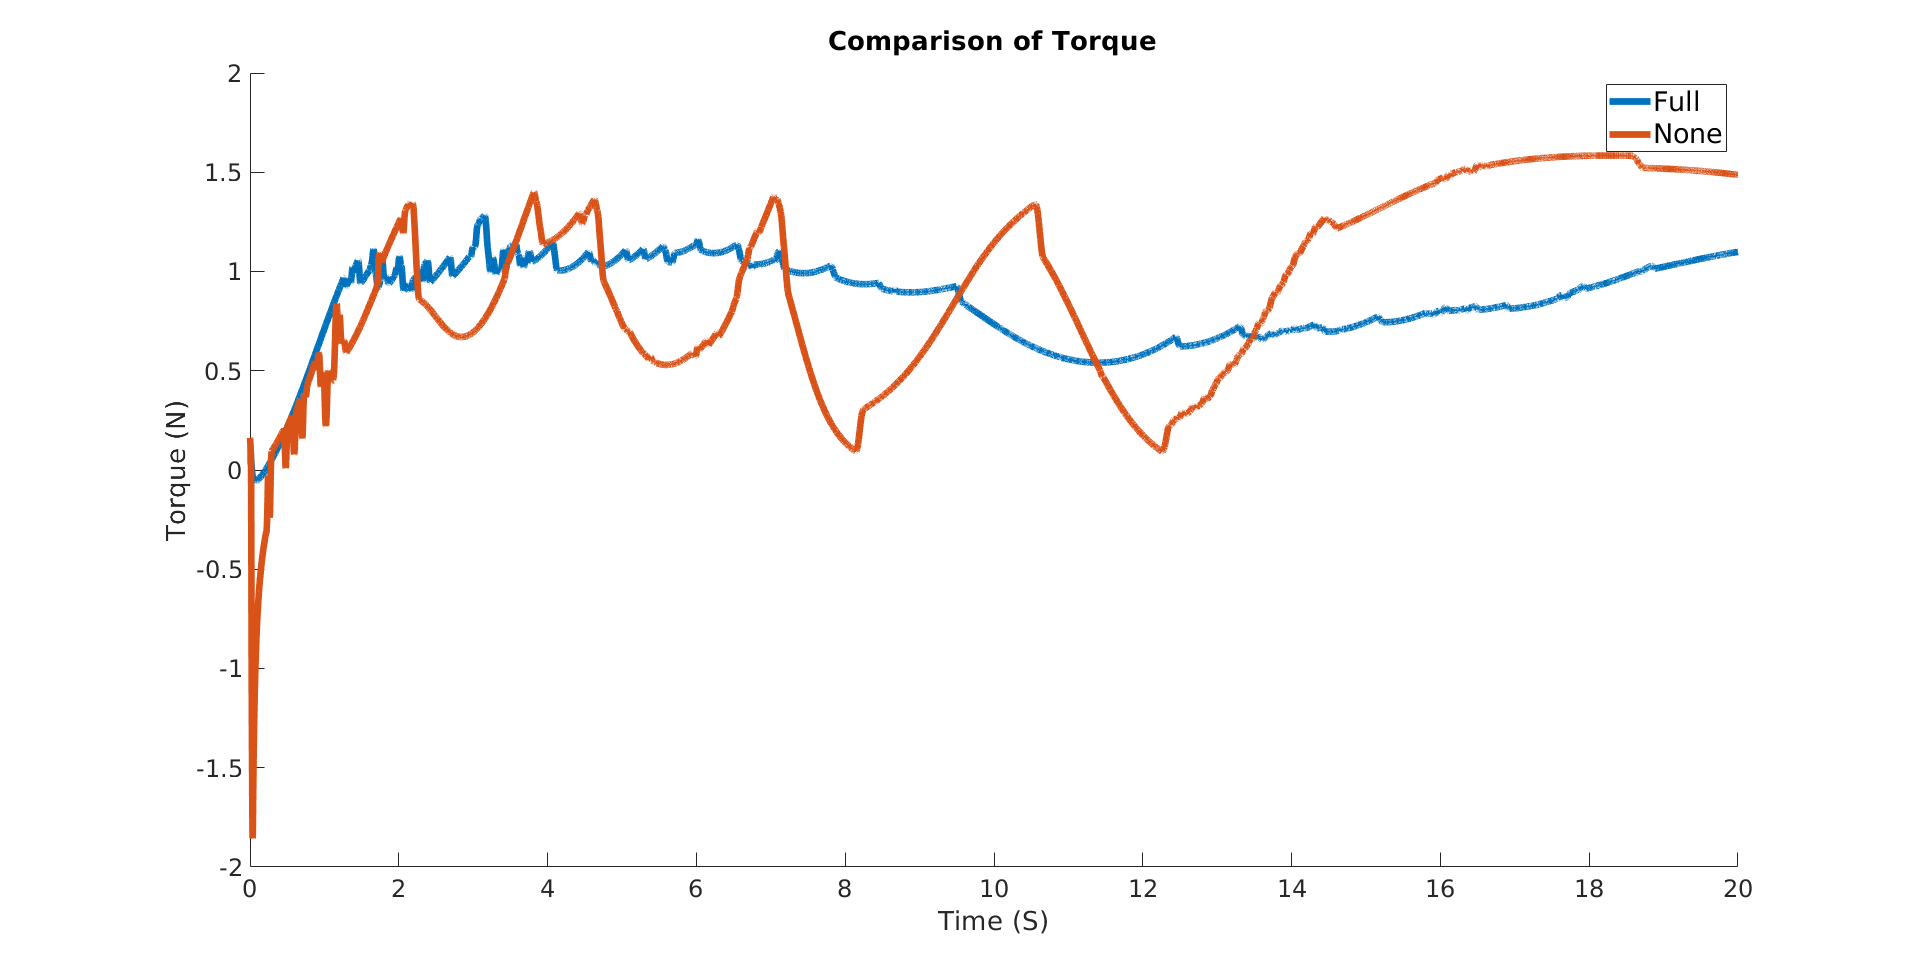
\includegraphics[width=\columnwidth]{images/controllers/comparisonOfTorque.png}
        \caption[Comparison of Torque for Full and No Engagement]{Comparison of a the torque on a physical system.}
        \label{fig:phyicalTorque}
    \end{subfigure}
    \caption[Physical System Engagement Levels]{Comparison of the torque profiles on the on the physical testing system.}
    \label{fig:phyicalSystemResults}
\end{figure}

 Application on real hardware comes with several challenges. Real systems must deal with sensor noise and communication speed, affecting how the controller responds to the model updates. This will improve the tracking error and smooth out the tracking signal displayed in both the  \textit{assistie}  and \textit{assistor} systems. These uncertainties need to be properly modeled to allow for offline tuning of the controller parameters. While the parameters for the physical system were tuned offline, they had the be slightly altered to handle the disturbance and friction in the system.  


\section{Contributions}

Several contributions were made to the field of controller development. The iLQR controller and the A-SMC cooperative controller introduced new methods that expanded previous applications and research. Both the controllers have applications outside the field outside of lower limb exoskeletons. The generalized forms of the controller can be used for assistive control applications and to generate optimal control signals for non-linear robotic systems. 


The iLQR controller introduced a new method of integrating an optimal controller with learning from demonstration to control a lower limb exoskeleton. This controller method allows a trajectory to be learned from multiple demonstrations and uses a non-linear dynamic model to learn an optimal control signal. Using a non-linear model allows the complex dynamics to be encoded into the control signal. The PD controller allows feedback to account for non-modeled dynamics. 

The new A-SMC was developed to handle a closed-loop controller attached to the assistive system; this builds upon the previous work that assumed the human controller was an open-loop controller. This closed-loop controller can be implemented as an FES controller on the user's leg muscles. Additionally, the standard interaction torques were generated using the iLQR controller, allowing optimal control commands to be used in the A-SMC. The controller was tested with various dynamic systems, various trajectories, and various involvement from the  \textit{assitie} system. The A-SMC controller was able to track the desired trajectories. 

The new tuning method of an A-SMC controller was presented, allowing for the parameters to be automatically determined. This method was shown to improve the state space of the SMC. Using a position and velocity cost function allows the gains to be automatically tuned to the system. This generalization of the tuning method allows it to be used for more complex systems with more joints or complex dynamics. Additionally, it was shown that the controller was able to handle varying alignment and involvements of the \textit{assitie} system; this is important since these controllers are often incorporated into \textit{assistive} exoskeleton systems. 

A sensitivity analysis was conducted to examine the importance of the A-SMC. This analysis showed the sensitivity of the controller, the parameter change, and what parameters have the largest effect on the tuning of the controller. Without this analysis, the A-SMC controller would be challenging to tune due to the many parameters in the controller since the numerous parameters scale with the degrees of freedom. Exoskeletons tend to have many degrees of freedom; therefore, this method is necessary for tuning and optimizing the controllers.   

The A-SMC controller was implemented on a dynamic model of a LARRE leg. This model has the same dynamics configuration as the simulated exoskeleton model. The dynamics model was used to train the controller using the methods described above to follow an arbitrary trajectory. These parameters were used to follow a gait cycle. It was shown that the controller was able to compensate for different levels of human involvement, including varying fatigue torque and no human involvement.   





